\documentclass[12pt, oneside]{book}
% % % % % % % % % % % % % % % % % % %
%
% USEPACKAGES; skept minimal, these can be amended but not removed.
%
% % % % % % % % % % % % % % % % % % %
\usepackage[table]{xcolor}
\usepackage{fancyhdr}
\usepackage{pdfpages}
\usepackage{graphicx}
\usepackage{mathtools}
\usepackage{amsmath}
\usepackage{hyperref}
\usepackage{makecell}
\usepackage{appendix}
\usepackage{listings}
\usepackage[margin=4cm, top=2cm, bottom=2cm, headheight=17pt, heightrounded,]{geometry}
\usepackage{float}
\usepackage{multirow}
\usepackage{pifont}
\usepackage{cite}
\usepackage{titlesec}
\usepackage{fancyvrb}
\usepackage{verbatim}
\usepackage{longtable}
\usepackage{filecontents,notoccite}
\usepackage[ruled,vlined, linesnumbered]{algorithm2e}
\usepackage{listings}
\usepackage{xcolor}
\UseRawInputEncoding
\definecolor{codegreen}{rgb}{0,0.6,0}
\definecolor{codegray}{rgb}{0.5,0.5,0.5}
\definecolor{codepurple}{rgb}{0.58,0,0.82}
\definecolor{backcolour}{rgb}{0.95,0.95,0.92}
\lstset{
   breaklines=true,
   basicstyle=\ttfamil
}
\lstset{
   breaklines=true,
   basicstyle=\ttfamily
}
\lstdefinestyle{mystyle}{
    backgroundcolor=\color{backcolour},   
    commentstyle=\color{codegreen},
    keywordstyle=\color{magenta},
    numberstyle=\tiny\color{codegray},
    stringstyle=\color{codepurple},
    basicstyle=\ttfamily\footnotesize,
    breakatwhitespace=false,         
    breaklines=true,                 
    captionpos=b,                    
    keepspaces=true,                 
    numbers=left,                    
    numbersep=5pt,                  
    showspaces=false,                
    showstringspaces=false,
    showtabs=false,                  
    tabsize=2
}
\lstset{style=mystyle}
\renewcommand{\lstlistingname}{Code Snippet}% Listing -> Code Snippets
\renewcommand{\lstlistlistingname}{List of \lstlistingname s}% List of Listings -> List of Code Snippets

\SetKwInput{KwRequire}{Requires}

\titleformat{\chapter}[block]
{\normalfont\huge\bfseries}{\thechapter}{1em}{\Huge}
\titlespacing*{\chapter}{0pt}{0pt}{10pt}
\titlespacing*{\section}{0pt}{7pt}{7pt}
\titlespacing*{\subsection}{3pt}{13pt}{3pt}
\titlespacing*{\subsubsection}{5pt}{10pt}{5pt}



% % % % % % % % % % % % % % % % % % %
%
% DEFINITIONS FILE
% Change Values of commands in file: "definitions-thesis.tex"
%
% % % % % % % % % % % % % % % % % % %
\newcommand{\studentNumber}{206059086}
\newcommand{\authorName}{Merlin Roe}
\newcommand{\thesisTitle}{Intrusion Detection and Prevention and Proxy Hybrid using Software-Defined Networking: ARP Poisoning Defence}
\newcommand{\degreeTitle}{MSc Cyber Security}
\newcommand{\moduleCode}{COM00097M}
\newcommand{\moduleTitle}{Project}
\newcommand{\moduleLeader}{}
\newcommand{\supervisor}{Vasileios Vasilakis}
\newcommand{\deptName}{Dept. of Computer Science}
\newcommand{\academicYear}{September 2020}

%\renewcommand{\thesection}{\Roman{section}}

\begin{document}

% % % % % % % % % % % % % % % % % % %
%
%	TITLEPAGE - DO NOT CHANGE
%
% % % % % % % % % % % % % % % % % % %
\begin{titlepage}
\begin{center}

	
\includegraphics[scale=0.5]{images/UniOfYorkLogo.png}


	\vfill

			{\huge \thesisTitle \\}

	\vfill

	\begin{tabular}{rl}
	Name: & \authorName \\
	Student Number: & \studentNumber \\
	Supervisor: & \supervisor \\
	Number of Pages: & 61\\
	& Including Abstract
	\end{tabular}
	\vfill

	A coursework submitted in fulfillment of the requirements\\ for the degree of \degreeTitle
	\vfill
	\deptName
	\vfill
	\academicYear
\end{center}

\end{titlepage}
\newpage

% % % % % % % % % % % % % % % % % %
%		HEADERS & FOOTERS
% % % % % % %. % % % % % % % % % % % %

\newpage



\pagestyle{fancy}
\rhead{\authorName}
\lhead{\nouppercase{\leftmark}}
\lfoot{\empty}
\cfoot{\thepage}
\rfoot{\empty}

% % % % % % % % % % % % % % % % % % % % % % % % % % % % % % % % % % % % % % % % % % % % % % % % % % % % % % % %
\frontmatter
\chapter{Abstract}
Software-Defined Networks (\emph{SDN}) are centrally and programmatically controllable networks, by decoupling
the control plane from the data plane on vertically designed routing devices.
Providing network-wide configuration and monitoring by the central
controllers and their associated network applications.

Intrusion Detection and Prevention Systems (\emph{IDPS}) are devices or software that are specifically designed
to monitor networks for malicious activity, taking preventative measures to prevent these actions and prevent
further activity from potential threats.

This report investigates and develops an innovative IDPS tailored to function alongside the SDN Ryu controller
specifically to detect and prevent a variety of ARP Poisoning attacks. By inspecting ARP packets within the network,
inserting specifically crafted Link Layer flow rules on an
Open vSwitch (\emph{OvS}) to actively forward or drop ARP requests and replies. The developed IDPS
utilises the network's DHCP server to maintain an autonomous host list, supporting static hosts via ARP packets.
The developed IDPS is a functioning hybrid between IDPS and ARP proxy,
by performing ARP replies for malicious devices that are blocked by the IDPS; ensuring traffic in false-positive scenarios.

Testing is carried out on a physical testbed, using an off-the-shelf TP-Link router with an OvS and an OpenFlow using
 several Raspberry Pi's as hosts,
resulting in real environment results. Three separate experiments were conducted on the IDPS using the physical
testbed. The first experiment tested the detection and mitigation with 400 total packets sent with 
a variety of ARP poisoning attacks, with prevention rate being \emph{100\%} and detected on average
within \emph{58.1ms}. The developed IDPS had minimal effect of regular ARP packets, only increasing by \emph{1.2ms}
on average with minimal impact on the Controller resources.

Future iterations of the IDPS expanding into IPv6 protocol by supporting the Neighbor Discovery Protocol (\emph{NDP}), 
supporting a growing range of IPv4 and IPv6 aware networks. Further utilising the DHCP offers by directly 
incorporating DHCP lease times into inserted flow rules \emph{hard\_timeout} flag, ensuring flow rules exist
for as long as IP and MAC pairings are valid.





\newpage
% % % % % % % % % % % % % % % % % % % % % % % % % % % % % % % % % % % % % % % % % % % % % % % % % % % % % % % %

\tableofcontents

\listoffigures

\listoftables

\lstlistoflistings

\newpage

\chapter{Abbreviations}

\begin{table}[H]
	\begin{tabular}{l l}
		\textbf{ARP}	 	& Address Resolution Protocol  \\
		\textbf{CSV}	 	& Comma-separated Values \\
		\textbf{CVE}	 	& Common Vulnerabilities and Exposures \\
		\textbf{DHCP}	 	& Dynamic Host Configuration Protocol \\
		\textbf{DoS}	 	& Denial of Service \\ 
		\textbf{DPI}	 	& Deep Packet Inspection \\ 
		\textbf{IDS}	 	& Intrusion Detection System \\ 
		\textbf{IDPS}	 	& Intrusion Detection and Prevention System \\
		\textbf{IP}	 		& Internet Protocol \\
		\textbf{MAC}	 	& Media Address Control \\
		\textbf{MiM}	 	& Man-in-the-middle \\
		\textbf{NAT}	 	& Network Address Translation \\
		\textbf{NIC}	 	& Network Interface Card\\
		\textbf{OvS}	 	& Open vSwitch \\
		\textbf{QoS}	 	& NQuality of Service \\
		\textbf{RL}	 		& Rate Limiting \\
		\textbf{RTT}	 	& Round Trip Time\\
		\textbf{SDN}	 	& Software Defined Network\\
		\textbf{TCP}	 	& Transport Control Protocol\\
		\textbf{UDP}	 	& User Datagram Protocol\\
		\textbf{VM}	 		& Virtual Machine \\
	\end{tabular}
\end{table}

%\chapter{Ethics Statement}
\chapter{Ethics Statement}
I, the author, Merlin Roe, declare that this report titled, {\thesisTitle} and
any work presented within it are original. I confirm that:

\begin{itemize}
	\itemsep0em 
  \item This work was done in candidature for a masters degree at the University of York.
  \item All source materials used have been acknowledged, whether they are directly quoted or not.
	\item The work has been completed in accordance with the University of York’s Academic Integrity Misconduct Policies, Guidelines andProcedures, which can be found at the following URL:
	      \newline\url{https://www.york.ac.uk/staff/supporting-students/academic/taught/misconduct/}
	\item Any assistance has been in accordance with the University’s Guidance on Proof reading and Editing and duly acknowledged. The latter document canbe retrieved from the following URL:\newline
	      \url{https://www.york.ac.uk/about/departments/support-and-admin/sas/student-related-policies/learning/}
	\item No part of this report has previously been submitted for a degree or any other qualification at this University or any other institution.
	\item In the case where source code has been developed from an existing script or template, this has been duly acknowledged.
\end{itemize}


% % % % % % % % % % % % % % % %
% CONTENT
% % % % % % % % % % % % % % % % % % % % % % % % % % % % % % % % % % % % % % % % % % % % % % % % % % % % % % % %
% % % % % % % % % % % % % % % % % % % % % % % % % % % % % % % % % % % % % % % % % % % % % % % % % % % % % % % %
% % % % % % % % % % % % % % % % % % % % % % % % % % % % % % % % % % % % % % % % % % % % % % % % % % % % % % % %
% % % % % % % % % % % % % % % % % % % % % % % % % % % % % % % % % % % % % % % % % % % % % % % % % % % % % % % %
% % % % % % % % % % % % % % % % % % % % % % % % % % % % % % % % % % % % % % % % % % % % % % % % % % % % % % % %
% % % % % % % % % % % % % % % % % % % % % % % % % % % % % % % % % % % % % % % % % % % % % % % % % % % % % % % %
\mainmatter
\chapter{Introduction}
The introduction chapter explains the importance of the project and offers a summary of
the overall system implementation and design.
This includes the context, motivation, objectives and the contributions this report provides.

\section{Context}
Due to the eruption of mobile devices, internet applications and cloud services, there have been significant
developments within computer networking. Many focus on the concepts of centralised programmable aware networks,
where an entire cloud service could be managed from a single central server.

Software-Defined Networks (\emph{SDN}) is an outcome of these developments as a new network architecture, which allows greater
control over the network by simplifying network management and reducing complexity \cite{feamster2013road}. The SDN
paradigm introduces a network controller as a new component within networks, this controller possesses omnipotent power
at managing the network. A network professional designs and configures the programmatically aware controller
by writing software specifically designed to control multiple packet forwarding devices using SDN defined protocols,
such as OpenFlow \cite{lara2013network}. The SDN paradigm has been exceeding adoption in many industries, for instance,
Google has deployed OpenFlow within its data centre backbone network to aid the utilisation on links carrying large
loads \cite{higginbotham2012}.
One study concluding significant SDN growth of 21.75\% per year within data centres and the
within the Internet of Things (\emph{IoT}) expansion \cite{tayyaba2016software}\cite{drutskoy2012scalable}. \newline

Given the surge of adoption for SDN (and OpenFlow) within industries, the importance of security within SDN
has grown. Research has been conducted into existing and new issues with regards to the SDN paradigm, introducing
new security solutions made
possible due to SDN and OpenFlow based environments. Particularly issues related to the
address resolution protocol \emph{(ARP)} poisoning attacks, which can be tackled in new ways relying upon the SDN paradigm.

ARP poisoning or ARP spoofing is an attack defined as the ability for an adversary to corrupt a hosts
IP to MAC address table for local networks. Whereby an adversary
pretending to be another device within
a network, such as manipulating hosts into using itself as the gateway of a
network. This allows an adversary to become the static route for all network traffic or a specific host, the attack 
is popular due to its simplicity to implement using the unauthorised ARP protocol \cite{nam2010enhanced}. ARP
spoofing is a serious attack which opens up the adversary to perform multiple types of attacks such as
Man-in-the-middle (\emph{MiM}), eavesdropping, MAC flooding and Denial of Service (\emph{DoS}).

% % % % % % % % % % % % % % % % % % % % % % % % % % % % % % % % % % % % % % % % % % % % % % % % % % % % % % % %
\newpage
\section{Motivation}
The vulnerabilities of ARP have been known since implementation, having been logged by
Common Vulnerabilities and Exposures \emph{(CVE)} as a possible DoS issue in 1999\cite{cve-1999-0667}; being scored a \emph{10}
for being one of the highest threats. ARP mitigation has continued to be a concern as the protocol still exists within
modern networks.
A well-known piece of malware called \emph{ServStart} relying on ARP poisoning has been used as recently as 2017 to
insert malicious adverts,
a server on a local subnet was compromised and the adversaries installed ARP spoofing malware
on the machine. The ARP spoofing malware poisoned the local network so outgoing traffic was forwarded through it,
the malware then inserted malicious JavaScript code into every HTML page served by hosts on the network\cite{doman_2017}.

Research detecting and mitigating ARP poisoning have started utilising SDNs central paradigm to maintain a paired 
list of MAC addresses and IP addresses of hosts on the local network, which aid in detecting when hosts are being
impersonated. The methods used for gathering and maintaining this list is vastly different, from researchers 
listening on and recording the ARP request and reply packets \cite{alharbi2016securing}, 
using the controller's own ARP Table \cite{matties2017distributed},
to relying on the Dynamic Host Configuration Protocol (\emph{DHCP}) \cite{masoud2015preventing}\cite{abdelsalam2015mitigating}.

The approach of a paired list is ideal as it becomes reference when detecting spoofed ARP packets, however, the research papers are
split on how to accomplish this. The ones utilising DHCP fail to determine DHCP offers are from a valid DHCP server,
allowing an adversary to push themselves onto the known list by acting as a valid DHCP server. These also fail to take into account previously configured hosts, and only one
supporting static IP addresses \cite{alharbi2016securing}.

The approach many of these papers take when testing their ARP poisoning mitigation's is to virtualise the environment
\cite{matties2017distributed}\cite{abdelsalam2015mitigating},
this creates unrealistic results when testing for the CPU load of the controller using the new algorithm, and affects
the Round Trip Time (\emph{RTT}) of packets due to lack of a physical network switch.
  
% % % % % % % % % % % % % % % % % % % % % % % % % % % % % % % % % % % % % % % % % % % % % % % % % % % % % % % %

\section{Objectives}
\label{sec:objs}
The objectives which this report will cover and attempt to accomplish, are based upon the previously 
discussed motivation and context around SDN networks. These are as follows:
\begin{enumerate}
	\itemsep0em
	\item Design and implement an IDPS system to detect and mitigate against ARP poisoning attacks using the SDN paradigm.
  \item Impose minimal effect on network speed and SDN controller resources.
	\item Test the IDS using a hardware testbed against a range of ARP poisoning attacks.
\end{enumerate}

% % % % % % % % % % % % % % % % % % % % % % % % % % % % % % % % % % % % % % % % % % % % % % % % % % % % % % % %
\newpage
\section{Project Contribution}
This report designs and develops an SDN based Intrusion Detection and Prevention System (\emph{IDPS}), specifically
for mitigating a variety of Address Resolution Protocol (\emph{ARP}) poisoning attacks; introducing a new hybrid approach
IDPS by incorporating an ARP proxy server to manage actively blocked MAC addresses.
The IDPS utilises the popular open-source Ryu SDN Controller and vendor adopted OpenFlow 1.3 protocol for communication to a 
physical SDN Open vSwitch (\emph{OvS}) switch.

Innovative new software was developed as an IDPS
operating as an extension to the Ryu controller, aiding in the decision of forwarding or dropping ARP packets.
The proposed system builds upon other papers such as \cite{alharbi2016securing}-\cite{masoud2015preventing}
which do not actively insert flow rules within the SDN paradigm, instead of handling
every ARP packet regardless of having been previously verified.
Therefore this system actively inserts flow rules to not only mitigate malicious packets, inserting flow rules which
forward verified packets, greatly reducing the CPU load and RTT of ARP packets.
While expanding on the research in\cite{masoud2015preventing},\cite{abdelsalam2015mitigating}, 
that utilises the DHCP protocol to verify and generate the network MAC and IP pairing, while adding support
for static IP addresses. The new hybrid IDPS, ARP proxy paradigm approach prevents
the possibility for an adversary to mask their MAC address as a known host, causing a false positive
IDPS blocking of a victim host. The hybrid approach ensures consistent replies from valid hosts
by the system using it's known host list to act as an ARP proxy, generating ARP replies.
The proposed system achieves this without any enhancements or modifications to the existing ARP protocol,
not requiring specialised software on individual existing or new devices, with limited strain on the SDN controller. \newline


The proposed IDPS is tested on a criteria of eight different signatures of poisoned ARP packets, consisting
of ARP requests and replies. The tests sent a total of \emph{400} poisoned ARP packets within the SDN network, were
all poisoned ARP packets amongst standard ARP were detected and dropped with the adversary MAC address being
actively blocked with a flow rule.
The testing highlights the average RTT for standard ARP is \emph{45ms}, IDPS flow rule ARP is \emph{46ms}
and being verified and forwarded by the proposed IDPS at \emph{96ms}. An insignificant
affect on the ARP RTT within the network, demonstrating the small interference the IDPS poses on the traffic.


% % % % % % % % % % % % % % % % % % % % % % % % % % % % % % % % % % % % % % % % % % % % % % % % % % % % % % % %
% % % % % % % % % % % % % % % % % % % % % % % % % % % % % % % % % % % % % % % % % % % % % % % % % % % % % % % %
% % % % % % % % % % % % % % % % % % % % % % % % % % % % % % % % % % % % % % % % % % % % % % % % % % % % % % % %
% % % % % % % % % % % % % % % % % % % % % % % % % % % % % % % % % % % % % % % % % % % % % % % % % % % % % % % %
% % % % % % % % % % % % % % % % % % % % % % % % % % % % % % % % % % % % % % % % % % % % % % % % % % % % % % % %

\chapter{Background} 
The background chapter contains the necessary information for the reader regarding potential unfamiliar concepts, tools 
and protocols. Initially discussing the differences between conventional networks and the programmable SDN paradigms,
followed by detailed explanations of software and tools used to manage and control an SDN; such as OpenFlow and OvSwitch.
This section also contains information about the specific tools and protocols used such as, the Ryu SDN Controller,
ARP protocol and IDPS.


\section{Conventional Networks}
Conventional computer networks are built up of many individual devices such as routers and switches,
with the primary purpose of sending, forwarding and receiving packets amongst themselves. These devices perform
their purpose by operating two functional planes: Control plane and Data plane. 
The Control plane is concerned with drawing the network topology, routing table, storing a list of destination
addresses and configurations defined by a network engineer whereby
it can act accordingly to define what to do with network packets. The Data plane forwards packets as defined
by the Control Plane to another device \cite{ramos2015software}. \newline

These devices function independently within large networks, with devices forwarding traffic based on their individual configuration,
and implementations. Therefore, devices decide how to forward each individual packet
according to their own routing tables, visible surrounding networks and configurations. Ensuring the network runs
predictably and reliably depends upon network engineers, who correctly and consistently configure these devices
with a clear understanding of the network and its complexity, as well as, the device is
functioning within \cite{caldwell2004cutting}.

\subsection{Problems with Conventional Networks}
As these devices are vertically integrated these planes are being controlled independently within each device, leading to
traditional computer networks becoming increasingly complex and hard to manage systems.

They involve different types of devices such as routers,
switches, network address translators, server load balancers, and intrusion
detection systems. Routers and switches usually run complex, distributed controlled software that is proprietary.

Network administrators are typically forced to configure individual network devices using configuration interfaces that
vary between vendors and different specific low level
configuration languages, even between different products from the same vendor. Although some network management tools
offer a central configuration for the network, these systems still operate with vendor-specific
protocols, mechanisms, and configuration interfaces.


While standard networking IP protocols emerge and develop, such as
Routing Information Protocol (\emph{RIP}) and Open Shortest Patch First (\emph{OSPF})\cite{rakheja2012performance}, vendors
often develop their own unique set of features and protocols designed to run on their systems.
Such as the Cisco Discovery Protocol (\emph{CDP})\cite{rodriguez2009topology}, used to share information between Cisco
specific devices. Vendors using different mechanisms cannot communicate with one another, resulting in extremely poor
interoperability between different devices.


Data centres are concerned that networks remaining reliable and
agile. Meaning they often focus on using devices from specific vendors which use proprietary
features and protocols, resulting in no solutions to the fundamental issue.
Vendors focus on extending the ability of their IP protocols on
their existing infrastructure, increasing the complexity with individually configured devices
making it difficult for new network architectures to emerge.

These fundamental issues of operation have increased
complexity and inflated both the capital and the operational costs of running a network, while
slowing innovation of network infrastructure designs such as Software Defined Networks
\cite{feamster2013road}\cite{benson2009unraveling}.

% % % % % % % % % % % % % % % % % % % % % % % % % % % % % % % % % % % % % % % % % % % % % % % % % % % % % % % %

\section{Software-Defined Networks}
\label{sec:SDNBASED}
\subsection{Programmable Networks}
The issues outlined within traditional networks are previously defined hurdles, aggravated over time, with new technology
and a shift to a more connected and cloud-based internet. The desire to move away from the
difficulty that vertically integrated devices bring, into programmable networks has been in slow development for
more than 20 years. Campbell et. al. researched the existing concepts for programmable networks in 1999
 as seen in \emph{'A survey of programmable networks'} \cite{campbell1999survey}.

The goal of programmable networks is to simplify the complexity of networking systems and allowing customers to
easily configure and introduce new services and protocols programmatically with 
their devices without being tied to the difficulties of specific vendors and their systems.

The concept of separating the Data plane and Control plane has been discussed in countless papers,
the Internet Engineering Task Force (IETF) began considering various ways to decouple the planes
and proposed the interface standard published in 2004 by Yang et. al. in
\emph{"Forwarding and Control Element Separation (ForCES)"}.\cite{yang2004forwarding}


\subsection{SDN Operation}
The development of programmable networks resulted in the current form of SDN;
an advanced and programmable approach to computer network architectures. Meaning the aforementioned concepts
to decouple the Control plane and Data plane.
The separation of these planes creates a new hierarchal layout using centralised
management and configuration over an entire network, the separation 
morphs network switches into simple forwarding devices and the Control plane is implemented within a
central controller, although in principle it is physically distributed. The central controller is the entity that
dictates the flow of traffic in the network.
The logical centralisation of the control logic is within a programmable software module
that runs in a standard server within the network. \newline

SDN offers a number of benefits, firstly, is it simpler and less
error-prone when modifying the network rules and policies, rather than via low-level individual
device configurations. Second, the central control program can automatically react to unforeseen changes and
continue to forward traffic within the network while maintaining the high-level
rules.
Third, the centralisation of the Control plane via a controller with global knowledge of the
topology and network state simplifies the development of newer and more advanced network functionality.
This ability to programmatically configure the network to Control the Data plane is the crucial feature of the SDN paradigm.
Providing new methods to solve age-old problems in networking, while simultaneously enabling
the use of sophisticated network rules and flows, such as security and dependability \cite{kreutz2013towards}.

\begin{figure}[h]
	\centering
	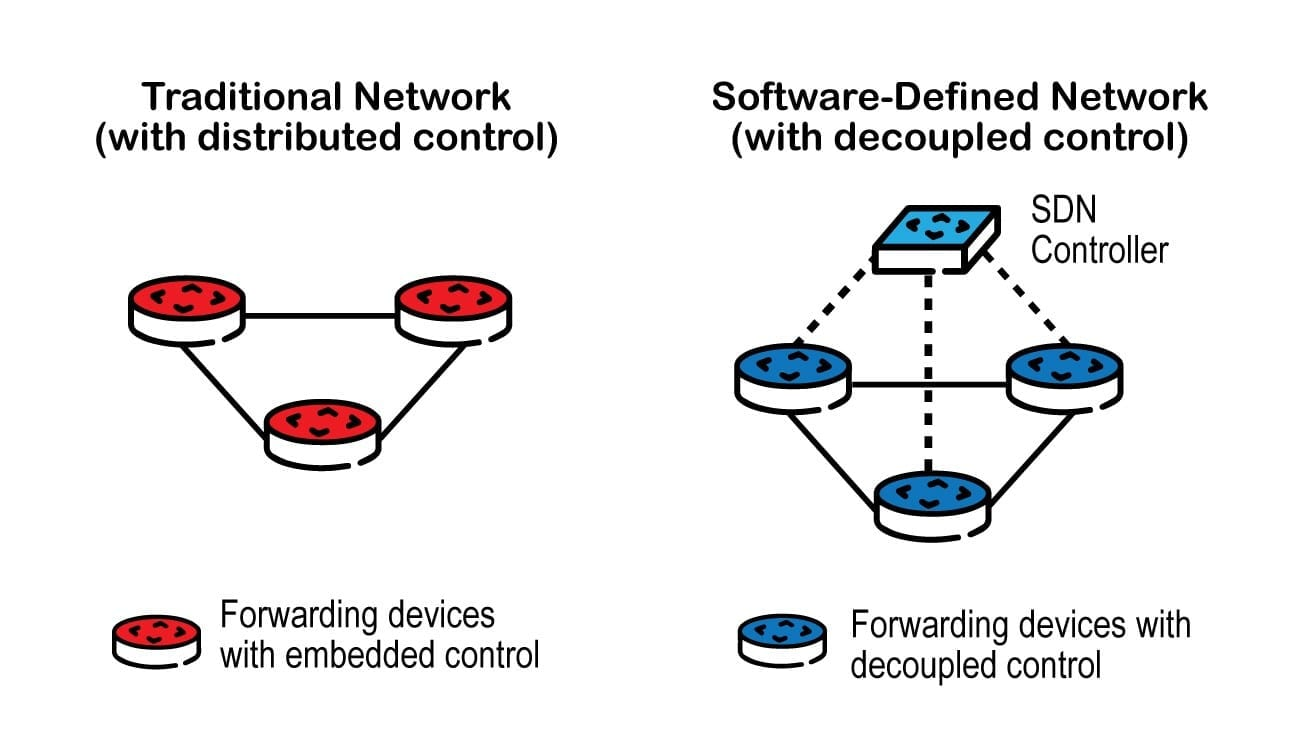
\includegraphics[scale=0.3]{images/sdnvtrad.jpg}
	\caption{Traditional Networks Compared to SDN \cite{SDNVTradImage2019}.}
	\label{fig:sdnvtrad}
\end{figure}

Figure \ref{fig:sdnvtrad} is the comparison of traditional networks and SDN, which visually
represents the switches communication with the central SDN controller. Whilst traditional networks devices
direct routes for individual packets, SDN devices use a new approach called flow tables.
Each routing device on an SDN has internal flow tables, as they receive unknown packets, it communicates with
the SDN controller 
to determine how the routing of said packet should be handled. The controller uses Deep Packet Inspection \emph{(DPI)}
to inspect the traffic in detail such as source address, destination address, protocols, etc. The controller
then creates flow rules based on the packet inspection, which the routing
device will then 
install and use for all subsequent packets that match the flow rule. Flow rule's offer the ability 
for routing devices to be instructed by 
a central server; how to route traffic without being relied on for all packets. A flow rule is generally built up
of the matching fields within a packet, such as a packet's protocol, source and destination,
and the action the switch must make on the packet; (i,e forward or drop).
 The controller will build up the flow tables within all the switches and routers to create a
unified network across routers, switches and firewalls, allowing network-wide configuration and flexibility\cite{kuzniar2015you}.

\subsection{Structure} % Components of SDN segments that build up a SDN network
An SDN structure is built up of several key components which are the decoupled planes in a traditional
network, as seen in Figure \ref{fig:sdnarch}\cite{sdnwebsite2020}.

\begin{minipage}{0.5\textwidth}
		
		\textbf{Application:} This application layer is where the software designed by a network engineer
		resides, this layer is where the programmable configuration software runs. Communicating with the
		controller via the controllers own dedicated API. \newline

		\textbf{Control:} The layer consists simply of SDN controllers, this software is what
		communicates with the network infrastructure (south-side) using an API such as
		OpenFlow\cite{mckeown2008openflow}, to the Application layer above. \newline

		\textbf{Infrastructure:} This encapsulates all the devices within the network that act within the Data plane, routing traffic,
		such as switches, routers and firewalls dictated by the Application via the controller. \newline

\end{minipage} \hfill
\begin{minipage}{0.40\textwidth}
	\begin{figure}[H]
		\centering
		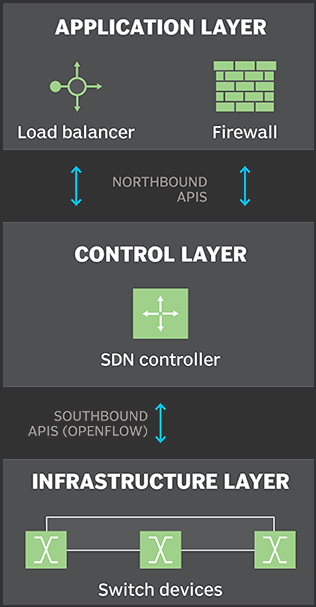
\includegraphics[scale=0.45]{images/sdn_architecture.png}
		\caption{SDN architecture \cite{rouse_2019}.}
		\label{fig:sdnarch}
	\end{figure}
\end{minipage}


\subsection{Controllers} % Controller purpose, options, focus on Ryu
Controllers are the primary component of an SDN, which as discussed dictates the networks behaviour.
The controller is what offers engineers the central programmable configuration, which communicates with switches over an 
API such as OpenFlow, \cite{mckeown2008openflow} which is discussed further in Section \ref{sec:openflow}.
There are several popular open source SDN controllers such as POX\cite{noxrepo_2012}, Daylight\cite{khattak2014performance},
ONOS\cite{berde2014onos} and Ryu\cite{ryusdnframework}, the proposed IDPS focuses on the Ryu controller as
discussed further in Section \ref{sec:ryuC}.

% % % % % % % % % % % % % % % % % % % % % % % % % % % % % % % % % % % % % % % % % % % % % % % % % % % % % % % %

\section{OpenFlow}
\label{sec:openflow}
This section covers OpenFlow and it's functionality within the SDN paradigm, this section refers to the
OpenFlow 1.3 documentation unless stated otherwise\cite{openflow}.

\subsection{Origin}
OpenFlow is a communications protocol which originated from a system called \emph{Ethane} proposed by Casado et. al.
at Standford University in 2007,
introducing simple flow-based ethernet switches with a centralised controller paradigm that manages the
forwarding and routing of traffic \cite{casado2007ethane}.
McKeown Et. Al. expanded on this idealogy in 2008 using Standford University’s network for testing, following Ethane, OpenFlow
was designed on the same concept \cite{mckeown2008openflow}. OpenFlow is a key role within SDN with enough momentum
to start the Open Networking Foundation \emph{(ONF)} in 2011\cite{openNF}.

\subsection{Operation} % What Openflow is in relation to SDN, basic design
OpenFlow a controller to access network switches or routers
to configure the forwarding plane and determine the flow of
network packets across networks and devices; as seen in Figure \ref{fig:openflowSwitch}.
An OpenFlow switch can contain one or more flow tables, performing 
packet matching for forwarding or communicating via the OpenFlow channel to the central controller. 
The switch communicates events to the controller and the controller manages the switch via the OpenFlow protocol.
The controller can then add, modify, and delete flow entries within the switches flow tables, both reactively
and proactively; leaving the actual forwarding of flow table matching packets to the switch at traditional speed for the duration
of those rules. Packets which do not match an existing rule within the switch are forwarded to the controller, can
then dictate where to be forwarded and if a flow rule is created. 

\begin{figure}[H]
	\centering
	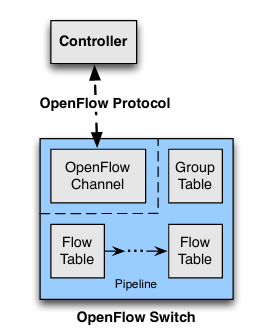
\includegraphics[scale=0.6]{images/openflow13.png}
	\caption{Main components of an OpenFlow switch \cite{openflow}.}
	\label{fig:openflowSwitch}
\end{figure}

\subsection{Flow Tables}% Basic buildup of Matching, instructions, and actions

The following Table \ref{fig:openflowTable} outlines the main components of a
flow rule within a table. Each flow table rule contains:

\begin{table}[H]
	\centering
	\begin{tabular}{|c|c|c|c|c|c|}
	\hline
	\textbf{Match Field} & \textbf{Priority} & \textbf{Counters} & \textbf{Instructions} & \textbf{Timeouts} & \textbf{Cookie} \\ \hline
	\end{tabular}
	\caption{Main components of a flow rule in a flow table \cite{openflow}.}
	\label{fig:openflowTable}
\end{table}

\begin{itemize}
	\item \textbf{Match fields:} On receiving an incoming packet the OpenFlow switch performs a lookup within the flow table to
				match the incoming packets fields and value's to a flow rule.
				These may also consist of the input port and packet headers.
	\item \textbf{Priority:} Incoming packets may match with multiple rules, therefore,
				each rule has a priority which the switch use to dictate it's actions.
	\item \textbf{Counters:} Each flow table, flow rule, port, queue, group, group bucket,
				meter and meter band, contain a counter which are updated when a incoming packet matches a flow rule.
				These values can be polled by a counter using the OpenFlow protocol.
	\item \textbf{Instructions:} Each flow rule contains an instruction that is executed when a packet matches the flow rules fields.
				These instructions result in changes to the packet routing, action set and/or processing, such as \emph{Apply-Actions}, \emph{Clear-Actions}
				or \emph{Write-Actions}.
	\item \textbf{Timeouts:} Flow rules contains a \emph{idle\_timeout} and a \emph{hard\_timeout}.
				The \emph{idle\_timeout} removes the flow rule once the 
				value reaches zero, which is set by the controller and is reset when a matching packet enters. The \emph{hard\_timeout}
				is set by the controller and simply applies the rule until the value reaches zero.
	\item	\textbf{Cookie:} Extra data included by the controller, can be used by the controller to
				filter flow statistics, flow modification and flow deletion.
\end{itemize}

An OpenFlow switch will contain a special flow rule for table misses, the flow rule ensures the switch can process incoming packets
that do not match any installed flow rules. The actions available to the flow rules can be either sending the packet to the 
controller to dictate how to proceed, drop the packet or forward the packet on its defined route.
The table miss rule does not exist by default and must be set by the controller or the OpenFlow switch itself, this rule
can be modified or deleted by the controller and may contain a timeout rule.

\newpage
\subsection{OpenFlow Channel}
The OpenFlow channel is the interface that allows communication between the OpenFlow switch and the controller.
This channel lets the controller configure and manage the switch, receive events, and send packets out the switch.
The OpenFlow channel doesn't offer any means of authentication, and therefore should be encrypted using TLS,
however, this is not enforced and may run directly over TCP\cite{openflow}.

The protocol supports three types of messages, controller to switch, asynchronous, and symmetric.
The proposed system utilises the controller to switch and asynchronous messages, the
key OpenFlow messages are described below:

\subsubsection{Controller to Switch}
Initiated by the controller and used to
directly manage or inspect the switch.
\begin{itemize}
	\itemsep0em
	\item \textbf{Feature:} The controller on establishment of the OpenFlow channel connection can request the identity
				and capabilities of the switch by a features request message. The controller uses this message to re-configure the
				switch with it's expected flow rules.
	\item \textbf{Modify-State:} These messages are sent from the controller to the switch to either
				add, delete or modify flow rules.
	\item \textbf{Read-State:} A mechanism introduced to allow the controller to collect various pieces of information,
				such as the configuration, statistics and capabilities of the switch.
\end{itemize}

\subsubsection{Asynchronous}
Asynchronous messages are initiated by the switch and update the controller of network events occurring within the switch.
\begin{itemize}
	\itemsep0em 
	\item \textbf{Packet-In:} When a table miss occurs, the switch can forward the incoming packet to the
				controller within a \emph{Packet-In} message.
	\item \textbf{Flow-Removed:} Informing the controller that a flow rule has been removed from the table, either
				from being deleted by the controller or due to a \emph{timeout} rule within the flow rule.
	\item \textbf{Error:} The switch can notify the controller of any errors it encounters.
\end{itemize}



\subsection{Version Comparison}
OpenFlow has seen several upgrades between the initial version 1.0 to version 1.5, the primary changes between versions
have been on the underlying architecture and flow table changes. Version 1.1 offering the addition of multiple tables per switch,
version 1.2 greatly increased the matching capabilities of the flow rules; introduction granularity flow tables.
OpenFlow 1.3 expands upon the matching possibilities and introduces the ability to support IPv6.
OpenFlow 1.3 has been widely adopted
by vendors such as HP supporting OpenFlow 1.0 and 1.3 in the \emph{HP 5920} switch series\cite{packard}.
The performance between the popular 1.0 and 1.3 OpenFlow versions as discussed by {\v{S}}ul{\'a}k et. al.\cite{vsulak2016performance},
discover that wider flow matching rules offer greater throughput, however, the narrow matching offered by OpenFlow 1.3 is greater
when using quality of service techniques; with negligible differences elsewhere.

As this project is implementing an ARP IDPS service, the advantage of installing granularity flow rules catered to specific
ARP requests and replies outweigh the higher throughput of ARP packets. Therefore when this paper refers to OpenFlow it's
referring to version 1.3, the difference in matching rules can be seen in the tables \ref{table:openflow10match} and \ref{table:openflow13match}
within the appendices.

% % % % % % % % % % % % % % % % % % % % % % % % % % % % % % % % % % % % % % % % % % % % % % % % % % % % % % % %

\section{Open vSwitch}
\label{sec:OvS}
The Open vSwitch (\emph{OvS}) is open source multi-layer virtual switch, it can operate as software within another machine;
such as inside a switch, router or virtual machine.
OvS is designed to enable network automation forwarding functions to programmatic extensions, while still supporting standard
management interfaces and protocols such as OpenFlow, NetFlow, sFlow, IPv6 and 802.1Q virtual LANS \emph{(VLAN)}.
OvS has been developed by a large open-source community that requires the ability for
transactional configuration database for C and Python bindings, offering more flexibility within the development of this project.
To support OvS, it comes with several beneficial tools to aid in the configuration and management of the switch,
such as \emph{ovs-ofctl} a utility for managing and configuring OpenFlow switches.
Alongside \emph{ovs-vsctl} used for managing and updating the configuration of the flow-based switch,
both tools aid in the setup and control of the switch\cite{openvswitch}.

As this report is implementing within the SDN paradigm it requires an OpenFlow compatible virtual switch, therefore, will be using
OvS as the software switch inside the router using OpenWRT which is discussed in the next Section \ref{sec:OpenWRT}.


% % % % % % % % % % % % % % % % % % % % % % % % % % % % % % % % % % % % % % % % % % % % % % % % % % % % % % % %

\section{OpenWRT}
\label{sec:OpenWRT}
OpenWRT is an open-source highly extensible Linux operating system targeted for embedded devices, typically for wireless routers.
Compared to vendor created operating systems which create a static firmware,
OpenWRT is a fully writable filesystem, with a dedicated resource package manager
called Open Package Management \emph{(OPKG)}.
OpenWRT removes the constraint of applications and configuration options forced by the vendor,
allowing the developer and user to customise the device through the use of the package manager and Linux based applications.
This offers the ability to install tools such as \emph{Arping}, \emph{Tcpdump} and \emph{Iproute2}, these are common and
affective networking tools which are used within this project. The \emph{OPKG} also contains the Open vSwitch package version \emph{2.11.3},
which supports OpenFlow 1.0 to 1.4 \cite{openwrtproject}.

A router powered by the OpenWRT operating system offers all the necessary tools, software and features required to be installed 
as a SDN switch.

% % % % % % % % % % % % % % % % % % % % % % % % % % % % % % % % % % % % % % % % % % % % % % % % % % % % % % % %
\newpage

\section{Ryu Controller}
\label{sec:ryuC}
The Ryu Controller is a component-based software-defined networking framework, written in Python3 it provides
components with a well-defined API that eases the development of creating new network management tools, control applications and
services. Ryu supports a variety of protocols for managing network devices, such as the OpenFlow protocol from version 1.0 to 1.5.
The API Ryu offers all the types of communication on the OpenFlow channel discussed in Section \ref{sec:openflow},
creating events within the proposed Python IDPS service, including full use of the matching flow fields required for this project.
As the Ryu controller is an ongoing project managed on \emph{GitHub}, while it  can be installed
through Python3's \emph{pip} command, this project opts to install Ryu through \emph{GitHub} to obtain the latest revision\cite{ryusdnframework}.


\subsection{Brief Controller Comparison}
As SDN has seen a large growth primarily within the community, there have been several popular community developed open source 
SDN controllers. Table \ref{table:controlleroptions} below is a brief comparison featuring a handful of popular projects:

\begin{table}[H]
	\centering
	\begin{tabular}{|
	>{\columncolor[HTML]{C0C0C0}}c |c|c|c|}
	\hline
	\textbf{Name}       & \cellcolor[HTML]{C0C0C0}\textbf{\begin{tabular}[c]{@{}c@{}}OpenFlow\\ Support\end{tabular}} & \cellcolor[HTML]{C0C0C0}\textbf{Language} & \cellcolor[HTML]{C0C0C0}\textbf{Latest Release} \\ \hline
	\textbf{Ryu}        & 1.0 - 1.5                                                                                   & Python                                    & 12/06/2020                                \\ \hline
	\textbf{POX}        & 1.0                                                                                         & Python                                    & 23/11/2017                                \\ \hline
	\textbf{NOX}        & 1.0                                                                                         & C++                                       & 14/02/2014                                \\ \hline
	\textbf{ONOS}       & 1.0 - 1.5                                                                                   & Java                                      & 02/06/2020                              \\ \hline
	\textbf{FloodLight} & 1.0 - 1.5                                                                                   & Java                                      & 19/06/2020                                \\ \hline
	\textbf{DayLight}   & 1.0 - 1.3                                                                                   & Java                                      & 25/03/2020                              \\ \hline
	\end{tabular}
	\caption{subset of Open source SDN Controller options.}
	\label{table:controlleroptions}
\end{table}

Due to NOX and POX being the earliest open-source SDN controller's developed by Stanford University, they have been used
in a variety of research papers\cite{alharbi2016securing}\cite{matties2017distributed}\cite{masoud2015preventing}.
These controllers have lacked development and have not been kept up to date with the Openflow protocol, only supporting
the initial Openflow version 1.0. Therefore, they lack newer performance advancements, matching field capabilities, multiple
table capability and security adjustments. Ryu has been chosen for this project due to constant updates, support of the 
latest OpenFlow Protocol, written in Python3 and is an open-source with community-driven documentation.

% % % % % % % % % % % % % % % % % % % % % % % % % % % % % % % % % % % % % % % % % % % % % % % % % % % % % % % %

\newpage
\section{Tools}
This section covers several tools that are used within the development and testing of the IDPS, this covers pre-existing
tools and utilities that are commonly used for networking and ARP spoofing.

\label{subsec:Scapy}
\begin{itemize}
	\itemsep0em
	\item \textbf{Iproute2:} Iproute2 abbreviated as (\emph{IP}) which is a collection of utilities for controlling and monitoring
    a series of aspects of networking within Linux, such as, routing, network interfaces, tunnels and traffic control \cite{hemminger}.
    Used within this report to alter network interfaces such as enabling promiscuous mode.
  \item \textbf{Tcpdump:} Tcpdump is a network packet analyser that runs via the command-line interface, relying on the 
    libpcap library it offers the visibility of TCP/ARP/IP and other packets being forwarded over a network \cite{richardson}.
    A key utility to test the SDN network as can view the network's traffic to determine if the SDN switch is
    correctly forwarding and dropping packets, generating \emph{pcap} files containing the network traffic.

  \item \textbf{Wireshark:} Wireshark is another network packet analyser that runs within a GUI, offering 
    many ways to view and filter a variety of protocols within network traffic. Wireshark can also read \emph{pcap}
    files created by Tcpdump\cite{wireshark}. This is used primarily to view and easily parse \emph{pcap} files generated
    by Tcpdump.

  \item \textbf{Arping:} Arping is a utility for probing hosts on a network, similar to \emph{ping} except
    probing by sending Link-Layer frames using ARP requests \cite{kuznetsov}. This is used when performing normal ARP requests,
    as well as spoofing ARP requests.
  % \item \textbf{Ettercap:} Ettercap is an open-source network security tool for simulating MITM attacks, which
  %   achieves the attack by performs ARP poisoning on the protocol \cite{ornaghiEttercap}. This tool comes with many options,
  %   which allows for extensive testing of the proposed IDPS.
  % \item \textbf{Iperf:} Iperf and Iperf3 have widely used networking tools designed to measure and tune networking performance.
  %   Iperf can create data streams to measure the data throughput between the two hosts in either or both directions\cite{dugan}.
  %    Used when testing data throughput during and prior to an ARP poisoning attack.
  \item \textbf{Python Scapy:} Scapy is a Python library that does packet manipulation\cite{Scapylib}. The library
    is used within the ARP proxy implemented within the IDPS, as well as a custom testing tool used to test a variety of ARP attacks.
  \item \textbf{Python PSUtil:} PSUtil is a Python library that performs system monitoring by retrieving information on
     system utilization (CPU, memory, disks, network)\cite{rodola}. Used by the proposed IDPS testing tool
     to gather CPU load while the IDPS is running.
\end{itemize}

% % % % % % % % % % % % % % % % % % % % % % % % % % % % % % % % % % % % % % % % % % % % % % % % % % % % % % % %
\newpage

\section{Address Resolution Protocol \emph{(ARP)}}
\label{sec:ARP}
The Address Resolution Protocol \emph{(ARP)} is a communication protocol defined in 1982 by RFC 826,\cite{plummer2008rfc}
used for discovering Link-Layer addresses (MAC address),
and the associated internet layer address, this report focuses on an IPv4 address.
This mapping is a critical function in the internet protocol
suite, as it enables hosts in a local network to communicate.

The structure of ARP packets is shown in Figure \ref{fig:arp_packet} which visually demonstrates
ARP encapsulated within an IPv4 network running within an Ethernet Frame.
The packet header specifies the type of protocol in use (ARP) at
each layer, as well as containing the operation code for ARP, request \emph{(1)} and
reply \emph{(2)}.
The primary payload of the packet contains four addresses, the hardware and protocol addresses of the source and target hosts.

\begin{figure}[H]
	\centering
	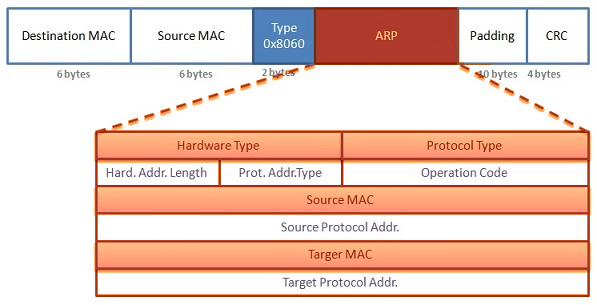
\includegraphics[scale=0.8]{images/arp-packet-format.jpg}
	\caption{ARP packet structure.}
	\label{fig:arp_packet}
\end{figure}

\subsection{ARP poisoning}
Due to the early development of ARP, security was an afterthought compared to speed,
therefore the basic security problem with ARP is that it's stateless, treating each request or reply
independently from any previous connection.
As a consequence, the ARP protocol has no method to authenticate the
sender of an ARP Request or Reply packet, or any means of checking the integrity and validity.

As a result, it is relatively simple for an adversary to broadcast an ARP request packet with forged source IP-MAC in the ARP header and Ethernet frame.
There are numerous ways to achieve this effect, such as the adversary using it's MAC address in the Ethernet Frame and the ARP header,
while using the IP address of its target, each attack relies on the misinformation
provided in the Ethernet Frame and the ARP headers.
When the target receives the spoofed ARP packet, it updates it may update internal ARP cache table with the attacker’s forged IP and MAC pair.
Therefore, when the target attempts to communicate with the original host, the packets will be destined to the MAC of the
adversary specified in the forged IP and MAC pair.
ARP poisoning may be used in several attacks, such as:

\begin{itemize}

  \item \textbf{DoS attacks:} The adversary can prevent communication between two or more hosts, also referred to as ARP flooding.
  \item \textbf{Host impersonation attack:} The adversary can receive packets destined for a host and impersonate and reply to these packets on their behalf.
        This can be achieved through the simple tool Arping, which is used for testing within this project by falsifying MAC address.
  \item \textbf{Man In The Middle (MITM) attack:} The adversary can monitor and save all the packets between two communicating hosts.
\end{itemize}

% % % % % % % % % % % % % % % % % % % % % % % % % % % % % % % % % % % % % % % % % % % % % % % % % % % % % % % %

\section{Intrusion Detection \& Prevention System \emph{(IDPS)}}
\label{sec:IDPS}
Traditional networks were designed with security in mind, specifically common network security involves
network firewalls, these devices protect networks by using a static set of rules to permit or deny network connections.
It implicitly prevents intrusions, assuming an appropriate and accurate set of rules have been defined outlining the attack.
Firewalls greatest limitation is its focus on 
limiting access between networks to prevent intrusion and do not detect or prevent an attack that originated within the network.
Intrusion Detection and Prevention Systems \emph{(IDPS)} controls the forwarding of traffic within and through a network and
protect it against adversaries, often IDPS are software applications designed to monitor networks by inspecting traffic for intrusion's
and taking the necessary action to prevent an attack. This form of detection allows a network to be secured from incoming
and outgoing traffic, as well as, internally forwarded traffic. Furthermore, the use of DPI does not rely on a specific set of static rules
like traditional firewalls, allowing the IDPS to function effectively in a changing network and threat landscape\cite{kenkre2015real}.


A Network Intrusion Detection and Prevention Systems (\emph{NIDPS}) is deployed at a strategic point within the network,
where it can monitor inbound and outbound traffic, to and from all the devices on the network\cite{scarfone2012guide}.
This is the type of IDPS the proposed system is following, relying on SDN to allow monitoring and altering
of traffic flow; as demonstrated in Figure \ref{fig:idpsSys}.

\begin{figure}[H]
  \centering
  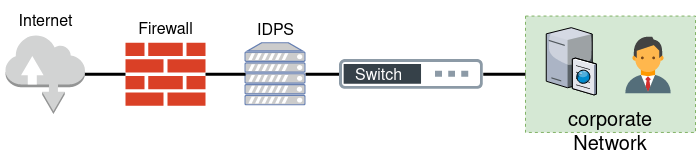
\includegraphics[scale=0.5]{images/IDPS.png}
  \caption{Intrusion Detection \& Prevention System Diagram}
  \label{fig:idpsSys}
\end{figure}

The IDPS performs a real-time deep inspection on every packet that is forwarded within the network,
detecting any malicious or suspicious packets, whereby it can perform one of the following actions:
\begin{itemize}
  \itemsep0em
  \item Dropping the related packets to the session detected exploiting traffic, block the offending source IP address or
        MAC address.
  \item Reprogram or reconfigure the firewall preventing an attack occurring again in the same format.
  \item Remove or replace any malicious content on the network during or following an attack.
        This is achieved by repackaging ARP payloads, removing header information deemed malicious and injecting safe information.
\end{itemize}



\subsection{Detection Methods}
IDPS typically employ the use one of three detection methods: signature based, anomaly based,
and stateful policy based:

\begin{itemize}
  \itemsep0em
  \item \textbf{Signature Based:} The approach uses predefined signatures of well-known network attacks. When an attack is detected that matches a known signature, the system takes necessary prevention action.
  \item \textbf{Anomaly Based:} This approach monitors for any suspicious or unexpected packets on the network. If an anomaly is detected, the system blocks access from the suspicious host device.
  \item \textbf{Policy Based:} This approach requires network engineers to configure specific security policies according to their given network infrastructure,
        an event which breaks a security policy is considered an attack.
\end{itemize}


% % % % % % % % % % % % % % % % % % % % % % % % % % % % % % % % % % % % % % % % % % % % % % % % % % % % % % % %
% % % % % % % % % % % % % % % % % % % % % % % % % % % % % % % % % % % % % % % % % % % % % % % % % % % % % % % %
% % % % % % % % % % % % % % % % % % % % % % % % % % % % % % % % % % % % % % % % % % % % % % % % % % % % % % % %
% % % % % % % % % % % % % % % % % % % % % % % % % % % % % % % % % % % % % % % % % % % % % % % % % % % % % % % %
% % % % % % % % % % % % % % % % % % % % % % % % % % % % % % % % % % % % % % % % % % % % % % % % % % % % % % % %



\chapter{Literature Review}
In this chapter, recent work regarding the security within SDN is researched,
initially looking into SDN security and IDPS solutions that have made a big impact or are still relevant despite bring older.
The focus shifts on recent and successful papers regarding the mitigation of ARP poisoning related attacks, using IDPS.
A comparison of these research papers is then briefly discussed, followed by a summary review of the papers and
the relationship to the project implemented in the rest of this paper.

\section{SDN security}
\label{sec:SDNSEC}
As SDN reaches a more stable position within its development,
research shifts from SDN design into more specific areas of its function; with a large focus on security.
The security research tackles a range of possible vulnerabilities, such as security exploits within the protocols a SDN may rely upon,
and using SDN to resolve existing network vulnerabilities to more elaborate issues and proposals, such as a distributed SDN system for
security; this section is dedicated into reviewing two papers related to SDN security.

\subsection{OpenFlow vulnerabilities}
This subsection is reviewing the paper by Samociuk, Dominik \cite{samociuk2015secure},
which explores the lack of security within the OpenFlow protocol.
Specifically, the OpenFlow Protocol handshake, which does not require the SDN controller to authenticate switches
and the controller is not required to authorise switches access to the controller.
This lack of security within the protocol itself
leaves it vulnerable to adversaries imitating a switch to access the controller, resulting in
DoS attacks that disrupt traffic.
Additionally, the lack of authentication and authorization in the OpenFlow handshake can be exploited by malicious switches
for covert malicious traffic, bypassing the Data plane and potentially Control plane security mechanisms.
One of the proposed solutions to resolving this lack of authentication is by the addition of Transport Layer Security \emph{(TLS)},
which ensures communication between the controller and switches are encrypted and authenticated.
OpenFlow, however, does not 
enforce TLS since version 1.1, instead only encourages the use of TLS.

Benton et. al.\cite{benton2013openflow} had researched the extent of this vulnerability within
existing controllers and switches by vendors which incorporate OpenFlow before Samociuk Dominik's paper.
Discovering and highlighting
that the vast majority of SDN implementations have a widespread failure of security, specifically due to the lack of TLS
within the control plane within the implementation of OpenFlow. 


\subsection{IDPS using SDN: Defending against port-scanning and DoS}
The vast majority of security research has taken advantage of SDN's ability to DPI,
the SDN controller inspects, in detail, the packets and their contents when being sent over the network. SDN relies on this functionality to generate
routing flows, therefore this existing feature means SDN is ideal for implementing
an IDPS by inspecting packets for malicious intent and deciding whether to drop, route or allow them. 
The paper by Birkinshaw et. al \cite{birkinshaw2019implementing}is one such paper that takes advantage of the SDN paradigm.

The team developed an IDPS within a SDN focusing on defence against port-scanning techniques and DoS attacks.
The team mitigated these threats by implementing and testing two connection-based techniques, namely the Credit-Based Threshold Random
Walk \emph{(CB-TRW)} and Rate Limiting \emph{(RL)}. Using these two techniques the team developed a new algorithm called Port Bingo,
designed to mitigate port-scanning attacks; furthermore using flow statistics 
alongside Quality of Service \emph{(QoS)} to mitigate DoS attacks. The team extensively tested these algorithms within a
purpose-built virtual testbed which consisted of an Open vSwitch, POX based controller and other hosts for
attackers and victims. \newline

The IDPS relies on DPI on received packets the controller obtains from the PacketIn event via the switch, to detect malicious intent
within the network traffic. The Port Bingo algorithm for detection and mitigation of port scanning consisted of the expectation that an adversary would send a large
number of packets to a large range of ports. Therefore, scanning the network traffic between pairs of hosts and comparing the ports to a list of prioritised port destinations, such as
80 for HTTP and 22 for SSH, in order of accessibility, would show any anomalies within the traffic.
An anomaly was considered when an accumulation of SYN packets sent to a host on these bingo ports, reached an accumulated value equal too or
higher than a threshold value, which had been building within a maximum period used for tracking. To avoid blacklisting a valid
machine, the tracked connection flow rule is deleted after a predetermined time.

Mitigation of DoS attacks was also achieved by relying on the Open vSwitch queueing on switch ports, which can be used to apply for QoS
flow entries. The algorithm developed would query the switch periodically to search for anomalies within the traffic by looking for excessive
byte count or packet count in either TCP, UDP or ICMP packets. Similar to the port scanning resolution, the algorithm implements
a flow rule to enqueue the offending packets on the egress switch port.

The Port Bingo TCP algorithm and QoS DoS mitigation successfully detected attacks, with correct flow entries automatically applied within offending switches
which drops the malicious packets.


\section{Related Work: SDN based ARP poisoning detection and prevention}
The following papers focus on ARP detecting and preventing
and shaped the development of this project, each subsection contains the paper's implementation,
the testing applied and a summary of limitations.


\subsection{Securing ARP in software defined networks}
\label{subsec:secureARPLIT}
A paper by Alhrabi et. al.\cite{alharbi2016securing}, proposes an algorithm
designed to mitigate ARP poisoning in IPv4 ARP which could be adapted to work on IPv6 Neighbor Discovery Protocol \emph{(NDP)}.
The paper's focal point is \emph{Regular ARP} over \emph{Proxy ARP}, where ARP is handled by the hosts themselves over the SDN controller
taking control and acting as a proxy server for ARP packets.
Their algorithm named \emph{'SARP\_NAT'} is loosely based on Network Address Translation \emph{(NAT)}. The IDPS relies on the
SDN controller receiving all ARP packets within the network for DPI.
The SARP\_NAT algorithm records the ARP requests into a pending list,
the algorithm NAT's the potentially malicious source MAC address and Protocol address turning the ARP request into a sanitised ARP 
request with dummy values which are then forwarded into the network. When the targeted machine replies to this ARP request the destination is broadcasted,
where the algorithm can authenticate using the ARP handled list. Once the algorithm has confirmed the ARP reply and request as 
valid, it can re-perform the MAC NAT to ensure the ARP packets have reached the correct destinations.

Testing was carried out on the SARP\_NAT algorithm using the POX SDN controller, with a linear topology containing 64 hosts and a tree topology
with a depth of 2 and 8 fanout for a total of 64 hosts. Several measurements were tested, the CPU load caused by the algorithm
over several different scenarios with an estimated reduction in CPU overhead of 22\%, as well as, the Round Trip Time \emph{(RTT)} which measured the time
to handle an ARP request. The test
demonstrated a significant speed advantage whereby, the ARP packets using the SARP\_NAT algorithm have a 32\% shorter RTT 
due to the \emph{l2\_learning} component for regular ARP packets.

The IDPS implemented in this paper proved extremely effective, however, the metrics used for the CPU load and RTT appear skewed.
The paper uses the \emph{l2\_learning} component of POX, which contacts the controller for all-new traffic adding a flow rules and
standard ARP request and replies due to the broadcasting nature of the protocol; making normal ARP behave slower.
The proxy element is also slightly slower due to the constant NATing of ARP request and replies as it does not actively insert flow
rules to speed up traffic.
Furthermore, the \emph{'SARP\_NAT'} algorithm can fall victim to spoofed gratuitous ARP replies,
receiving two ARP replies with different values in the source MAC address field,
one from the genuine target host, and one from the attacker. Unfortunately, the \emph{'SARP\_NAT'} component cannot determine
which one is the genuine reply and which one is poisoned.





\subsection{Distributed responder ARP: Using SDN}
\label{subsec:DistPaperLIT}
As briefly mentioned in the above discussed paper, this paper utilises the concept of an \emph{Proxy ARP},
\emph{Distributed Responder ARP: Using SDN to re-engineer ARP from within the network} by Mark Matties takes\cite{matties2017distributed}.
The paper uses a SDN to create an architecture using a service called Distributed Responder for ARP \emph{'DR-ARP'}, while other papers
focus on using the SDN controller as an IDPS; this paper uses the SDN primarily for the routing feature in the flow tables.
DR-ARP runs as a separate Python service.

Switches are inserted with a set of flow rules that forward ARP requests into the DR-ARP responder service, 
which maintains an ARP service table; consisting of the standard ARP table containing pairs of MAC address to an expected IP address,
plus meta-data on all ARP transactions. The DR-ARP then transmits the newly crafted and valid ARP replies, which the
SDN network forwards directly to the requesting host's ARP. Depending on the load and network scale, the service may be 
a single responder or distributed across multiple responders; which can update each other's ARP service tables.
If the service fails to find a matching host in its tables
for the ARP request, the service itself sends an ARP request expecting the host itself to reply to update it's local ARP service table.
This design prevents an adversary from poisoning ARP with an ARP request replay attack as the service acts as an authenticating ARP proxy
demonstrated in Figure \ref{fig:dr-arpLIT}.

\begin{figure}[H]
  \centering
  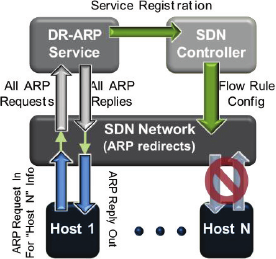
\includegraphics[scale=0.62]{images/dr_arpLIT.png}
  \caption{Distributed Responder ARP Architecture \cite{matties2017distributed}.}
  \label{fig:dr-arpLIT}
\end{figure}

Testing was performed within a virtual network on a single machine, using namespaces with ping processes to simulate machines with their own 
ARP tables. The DR-ARP responder was successfully in acting as an ARP proxy and limiting and validating ARP calls, by dropping invalid ARP packets.
This service greatly increased the RTT of the ARP requests from 1ms to 6ms, the author summed this up in part due to
inefficient speed a separate Python service using libpcap library to DPI the ARP requests. This implementation also has no ARP flood
protection and relies on regular ARP to discover new hosts for it's internal ARP table, which could be poisoned directly to the service
causing all subsequent ARP replies from the proxy to be incorrect.

%Limitations
%- Virtual Testing
%- Relies on Proxy ARP, if unknown ARP, Controller asks slower (x2 arp)
%- No ARP flood protection
%- Does not handle if ARP impersonates a valid MAC address, attempting to have MAC from valid host blocked



\subsection{Preventing ARP poisoning attack utilizing SDN paradigm}
\label{subsec:preventARPLIT}
Masoud et. al. proposes a new algorithm aimed in detecting and mitigating ARP poisoning for a network regardless whether hosts are 
assigned a dynamic \emph{(SDN\_DYN)} or a static IP address \emph{(SDN\_STA)}\cite{masoud2015preventing}.

The algorithm detects the SDN\_DYN hosts by inspecting the DHCP packets between the DHCP server and hosts, registering hosts paired
MAC address and IP address; handed to them by external the DHCP server.
Ensuring static IP SDN\_STA addressed machines are addressed, the algorithm monitors new traffic and detect hosts that 
do not have an existing match within the known hosts table. This paper is the only one that maps the network's topology
automatically and accurately registers static IP addressed hosts.
Using the list of hosts gathered from SDN\_DYN and SDN\_STA the algorithm residing within a Ryu SDN controller inspects
all ARP reply packets, if the IP address or the MAC address contained in any ARP reply is not the same as the recorded mapped value; 
the reply is dropped.


Masoud et. al. tested the algorithm on the physical HP-2920-24G switch with SDN enabled, using physical machines connected to 
the SDN with a mix of Linux and Windows as seen in Figure \ref{fig:Fuck}. While using the open-source Ryu SDN controller t
manage the new algorithm, and an external DHCP server.
The team used the software Cain and Abel \cite{cainandabel} to perform the ARP 
poisoning, which managed to assert their algorithm, mitigating all ARP spoofing attacks\cite{masoud2015preventing}.

\begin{figure}[H]
  \centering
  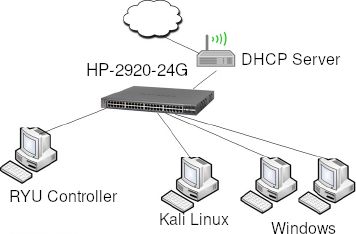
\includegraphics[scale=0.6]{images/hp_layout.png}
  \caption{Physically Tested setup \cite{masoud2015preventing}.}
  \label{fig:Fuck}
\end{figure}

The paper introduces an interesting approach utilising the DHCP server to detect new hosts on the network, however, the paper
does not take into account the validation of the DHCP server; as it may be possible to run a malicious DHCP server to produce
false-positive MAC and IP pairings. The paper also makes a point to indicate that all ARP replies and requests are forwarded to the 
controller forwarding each validated ARP packet; any subsequent packets need to be re-validated and no flow
rules are actively inserted within the switch. This slows down the ARP traffic and flood the controller due to the constant
re-validation, rather than inserting a rule for the valid replies.

% Limitations
%- Does not add flow rule for replies, E.G every reply is monitored regardless if previously determined safe - Slow
%- No DHCP validation, could impersonate the DHCP server to make controller think are valid.
%- Large overhead during ARP Flood due to handling all ARP packets and only dropping if unmatched



\subsection{Mitigating ARP Spoofing Attacks in SDN}
\label{subsec:mitigateARPLIT}
The following paper by Abdel Salam et. al. \cite{abdelsalam2015mitigating},
proposes a similar solution to ARP poisoning mitigation as the prior paper by Masoud et. al. The team focused on using the POX SDN
controller with the \emph{l2\_learning} module.
On startup they implemented flow rules to the SDN switches forwarding all ARP and DHCP packets directly to the controller.
The controller is designed to monitor the DHCP traffic, upon the DHCP offering an IP address to a host; to then track the paired MAC
and IP addresses into a known host list. ARP requests and reply packets received by the controller
are regarded as spoofed by the IDPS if their source or destination
ethernet header differs from the known host list, or if the controller receives an ARP with a MAC address that is not within it's known host
list and dropped. To further protect the SDN, the team implement a controller DoS protection which is similar to a QoS.
The implemented controller monitors the ARP throughput on each interface to detect anomalies in ARP traffic, this is achieved by counting the 
ARP packets; when a large amount is detected the controller implements a rule to temporarily drop traffic from the offending interface.
If any of these stated situations occur, the controller registers the event as an attack signature,
installing a flow rule on the switch, preventing further incoming traffic.

The POX controller was tested within a virtual Mininet\cite{mininetwebsite} network on a virtual machine, with a range of ARP attacks.
The testing results indicated success in mitigating the attacks with a negligible load on the CPU of the controller,
the ARP DoS flood was detected within \emph{0.7} seconds while the ARP request and reply attack were detected within around \emph{0.100} milliseconds.
The implemented solution ensured throughput speeds dropped only by a fraction from \emph{77.9} Mbps to \emph{72.2} Mbps during an ARP flood,
compared to the throughput without any protection.

Similar to the prior paper this implementation utilises the DHCP server, however, it does not take into account static IP addresses
unless explicitly defined by the user within the known host's file.
The paper also fails to indicate if the DHCP server is validated, leaving it vulnerable to a malicious DHCP server to produce
false-positive MAC and IP pairings. The flow rules installed by the controller drop all traffic from the host,
the adversary could inject poisoned ARP packets using a known host's MAC address. Using the controller to block the MAC address
of a valid host as a form of DoS attack using the ARP protocol.


% Limitations
%- Virtual Testing
%- Only DHCP - no static 
%- No DHCP validation, could impersonate the DHCP server to make controller think are valid.
%- Does not handle if ARP impersonates a valid MAC address, attempting to have MAC from valid host blocked


\newpage
\section{ARP IDPS Summary and Comparison}
\subsection{Comparison}
Referring to Table \ref{table:IDPSComp} the papers researched all utilise SDN in some form to mitigate and prevent ARP poisoning,
primarily using the SDN's central controller as a DPI
to examine packets, mitigating ARP spoofing by dropping or forwarding rules for specific hosts. The exception being Mark Matties
\cite{matties2017distributed}, in
 which it runs alongside the controller installing flow rules initially to have DHCP and
ARP packets forwarded to itself, then acting as a proxy ARP server by handling ARP replies itself. Only Abdel Salam et. al. \cite{abdelsalam2015mitigating}
actively installs flow rules within switches to drop or forward packets for the future, with the other three opting to receive or drop all 
within the controller, which increases the controller's processing requirement.

\begin{table}[H]
	\centering
	\begin{tabular}{|l|c|c|c|c|}
		\hline
		\rowcolor[HTML]{C0C0C0} 
		\textbf{IDPS features}  &  \cite{alharbi2016securing} & \cite{matties2017distributed} & \cite{masoud2015preventing} & \cite{abdelsalam2015mitigating} \\ \hline
		\textbf{Utilises DHCP server}                                                   &   &   & X & X \\ \hline
		\textbf{\begin{tabular}[c]{@{}l@{}}Supports Static IP\\ Addresses\end{tabular}} & X & X & X &   \\ \hline
		\textbf{ARP spoofing mitigation}                                                & X & X & X & X \\ \hline
		\textbf{ARP Flood protection}                                                   &   & X &   & X \\ \hline
		\textbf{Acts as proxy ARP}                                                      & X & X &   &   \\ \hline
		\textbf{Actively inserts flow Rules}                                            &   &   &   & X \\ \hline
	\end{tabular}
	\caption{ARP SDN IDPS Design and functionality comparison}
	\label{table:IDPSComp}
\end{table}

The testing carried out within these research papers differs vastly, this is seen in Table \ref{table:IDPSTestingComp} which summaries
the testing environment and the type of metrics gathered during testing.
Two papers \cite{masoud2015preventing}\cite{alharbi2016securing} implement and test
the ARP IDPS within a physical testbed, with other papers opting to virtualise the environment.
However, these papers lack testing metrics, instead of focusing on whether it's successful or not in mitigating a Man-In-The-Middle
attack.
The other three papers used a variety of metrics, such as the RTT, Detection time and most interestingly
paper \cite{abdelsalam2015mitigating} tested data throughput; where they test the traffic throughput between hosts during
an active ARP attack. This testing demonstrates the effect an ARP attack could have on the performance of the host itself,
rather than on the controller.

\begin{table}[H]
	\centering
	\begin{tabular}{|l|c|c|c|c|}
		\hline
		\rowcolor[HTML]{C0C0C0} 
		\textbf{Environment / Testing}  & \cite{alharbi2016securing} & \cite{matties2017distributed} & \cite{masoud2015preventing} & \cite{abdelsalam2015mitigating} \\ \hline
		\textbf{Physical testbed}        &        X              &                       &           X           &                       \\ \hline
		\textbf{Virtual testbed}         &                       &          X            &                       &            X          \\ \hline
		\textbf{ARP mitigation Testing}  &        X              &          X            &           X           &            X          \\ \hline
		\textbf{CPU Load Testing}        &        X              &                       &                       &            X          \\ \hline
		\textbf{RTT Testing}             &        X              &          X            &                       &                       \\ \hline
		\textbf{Data throughput Testing} &                       &                       &                       &            X          \\ \hline
		\textbf{Detection Time Testing}  &                       &                       &                       &            X          \\ \hline
	\end{tabular}
	\caption{ARP SDN IDPS Test environment and metrics}
	\label{table:IDPSTestingComp}
\end{table}

\subsection{Summary}
The papers \cite{matties2017distributed}\cite{masoud2015preventing}\cite{abdelsalam2015mitigating} all maintain a list of known hosts
comprised of the MAC address and IP address, the solution has been widely used and gives the controller a list to authenticate against.
However, only \cite{masoud2015preventing}\cite{abdelsalam2015mitigating} utilises the DHCP server to aid in the creation of the known
hosts,
yet, do not validate the DHCP packets themselves, this report's proposed system developed a mechanism
to verify the DHCP offers.
Another issue raised when relying on the DHCP server is the use of 
static IP addresses, only \cite{masoud2015preventing} appears to accommodate for this situation. The IDPS outlined in this paper
uses a similar approach in regards to building the network topology utilising DHCP server and supporting static IPs.\newline

The paper by Abdel Salam et. al. \cite{abdelsalam2015mitigating} utilises the SDN paradigm of actively installing
new flow rules within the switches,
whilst the other's constantly receive all ARP packets for forwarding or dropping. Requiring to re-authenticate
ARP requests and replies causing overhead on the controller, subsequently impeding on the RTT of the ARP packets, due to the forwarding 
through the controller. These papers likely used the older OpenFlow protocol 1.0 which does not support some key flow rule matching
capabilities that OpenFlow 1.3 supports such as ARP specific rules, see Section \ref{sec:openflow}.
The proposed IDPS resolves the issue by using the newer OpenFlow 1.3 matching fields, which can match ARP packets directly,
discussed in Section \ref{sec:openflow}. Installing
a flow rule for an ARP reply that has been verified reduces traffic to the controller while ensuring a low RTT for ARP,
mitigating the stated issues while ensuring the ARP replies are valid.\newline

The examined papers mix between proxy ARP \cite{alharbi2016securing}\cite{matties2017distributed} and
regular ARP\cite{masoud2015preventing}\cite{abdelsalam2015mitigating}. Proxy ARP offers the advantage of always receiving
ARP replies from a valid source, depending on how the proxy builds it's known MAC list. However, it requires larger overhead due to
validating and
replying to all requests. Whilst the regular ARP has less overhead after authenticating, yet relies on hosts to request and reply
to one another. The proposed system remedies this by using a hybrid of the two implementations, relying on regular ARP between hosts
using the central
IDPS to validate and install flow rules, however, to avoid the issue highlighted in the examination of paper
\cite{abdelsalam2015mitigating}
where a MAC address that's blocked can result in a false-positive block of a valid MAC address. The controller
temporarily acts as an ARP proxy server for blocked host using the known host list. \newline

Research is often carried out in an easier to obtain virtual environment on standard machines,
however, both \cite{alharbi2016securing} and \cite{masoud2015preventing} tested using a physical testbed. This approach
gave the research teams more accurate testing results and expectations of their algorithms in real-world settings,
this system follows the same methodology of testing the IDPS on real hardware; this offers more accurate results and 
accurate testing of the CPU load on the controller.


% % % % % % % % % % % % % % % % % % % % % % % % % % % % % % % % % % % % % % % % % % % % % % % % % % % % % % % %
% % % % % % % % % % % % % % % % % % % % % % % % % % % % % % % % % % % % % % % % % % % % % % % % % % % % % % % %
% % % % % % % % % % % % % % % % % % % % % % % % % % % % % % % % % % % % % % % % % % % % % % % % % % % % % % % %
% % % % % % % % % % % % % % % % % % % % % % % % % % % % % % % % % % % % % % % % % % % % % % % % % % % % % % % %
% % % % % % % % % % % % % % % % % % % % % % % % % % % % % % % % % % % % % % % % % % % % % % % % % % % % % % % %


\chapter{Design \& Implementation}
\label{Chap:DesImp}
This chapter defines the functionality of the project in its entirety,
covering the purpose, overview, project requirements, philosophy on utilising methods from prior research papers
and designing a new system to mitigate
ARP poisoning, accompanied by a high-level design of the IDPS.

\section{Purpose}
The purpose of the proposed IDPS system, which is an extension to an SDN controller, is to detect a
variety of ARP poisoning attacks that are then prevented, finally mitigating further attacks
launched by the adversary via blocking the intruding MAC address from transmitting
ARP packets. The proposed IDPS takes full advantage of the SDN flow tables unlike the prior researched papers
\cite{alharbi2016securing}-\cite{abdelsalam2015mitigating}, by actively inserting flow rules for specific
verified ARP packets rather than the conventional method of forwarding and re-validating all ARP packets within the IDPS.
Furthermore, this IDPS system proposes a new hybrid paradigm of ARP IDPS and ARP proxy. Whereby relying on the IDPS 
to detect poisoned ARP packets, actively inserting 
flow rules to forward all pre-verified packets and an ARP proxy to manage blocked MAC's ARP traffic to ensure 
other traffic is not impeded, preventing an adversary from causing a false-positive ARP block on a victim host.
Papers \cite{alharbi2016securing}\cite{matties2017distributed} rely solely 
on an ARP proxy as mitigation, ARP proxies handle all ARP packets, slowing 
down the RTT for ARP while requiring a large overhead on the device to handle the traffic.
The goal of the hybrid paradigm counters the disadvantage by
relying on an ARP proxy for a small subset of packets, preventing DoS via false-positives  while minimising the overhead.


\section{Operation Overview}

Figure \ref{fig:idpsflow} is a high-level flow chart that covers the overview in a visual representation,
the implemented IDPS code is available within Appendix \ref{app:IDPScode}.
The IDPS functions by using a \emph{mac\_knownlist}, a paired list of known devices on the network,
containing the MAC address, last known IP address and the IP origin; DHCP, Static or Unknown.
This list enables the IDPS to cross-reference ARP packets to known hosts, 
aiding in detecting ARP packets attempting to spoof other devices.
The IDPS initially sets SDN switches to forward all ARP and DHCP packets directly to the controller,
with the default table-miss flow rule to forward traffic as a normal switch; this default rule allows all other
traffic to flow like a traditional network and not impede on normal traffic; while minimising
the number of packets the controller processes. The IDPS awaits two events, \emph{PacketIn},
when a switch receives an ARP or DHCP packet and \emph{FlowRemoved}, when a flow rule is removed from \emph{idle\_timeout}
flag trigger. 

The DHCP packets are used to update the \emph{mac\_knownlist}, by observing
the DHCP IP address offers, the IDPS keeps an updated list of devices and their IP addresses. The DHCP server is also validated,
using DPI to verify the MAC and IP address of the DHCP server, which is stored within \emph{dhcp\_whitelist}.
These packets are inspected and forwarded, only dropped when a DHCP offer from an unverified DHCP server is detected.

When an ARP packet enters the controller, a check on the packet's MAC and IP address to
the \emph{mac\_knownlist} is performed, if new and unused MAC and IP addresses are present, it's then added to the list as a static IP.
ARP packets go through a series of DPI validations to detect any potential ARP poisoning methods, see \ref{table:reqARPpos}.
An ARP packet that has been verified
gets forwarded back into the network and functions as regular ARP. A flow rule matching the specific verified ARP packet with an 
\emph{idle\_timeout} is inserted on the switch. Actively inserting flow rules for verified ARP packets prevents the controller from
resource deprivation by re-validating packets,
the idle timeout is added to support the changing MAC and IP allocation by the DHCP. If, however, the ARP packet is 
considered malicious, the IDPS drops the packet and actively insert flow rules to drop any ARP packets from the
MAC address; this again includes an idle timeout for similar reasons. During which the IDPS controller acts as an ARP proxy,
replying to the blocked MAC ARP requests using the MAC and IP pair stored in the \emph{mac\_knownlist}; this is to prevent DoS attacks,
where an adversary produces a false positive ARP block by having valid hosts MAC address blocked.

\begin{figure}[H]
	\centering
	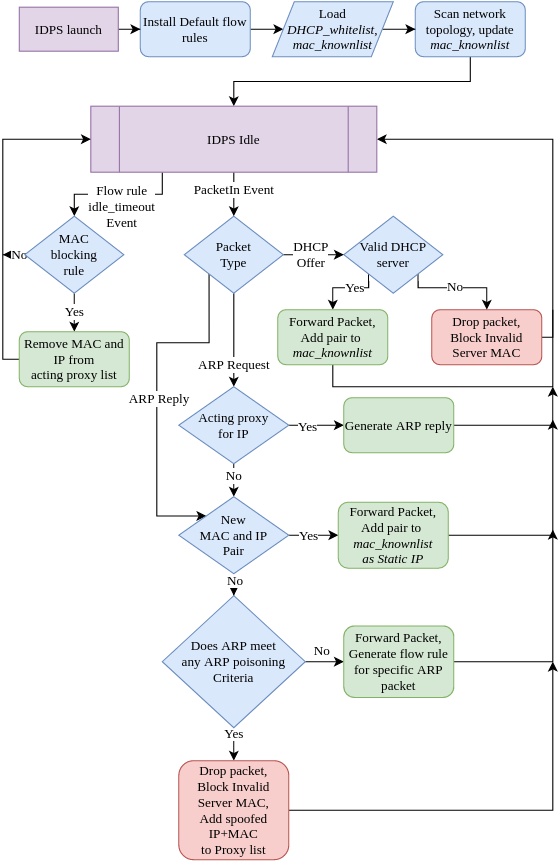
\includegraphics[scale=0.67]{images/IDPSflow.png}
	\caption{IDPS Flow-Chart}
	\label{fig:idpsflow}
\end{figure}

\newpage
\section{Feature Requirements}
The requirements listed in Table \ref{table:reqFeature} are key components and features that are required
to achieve the desired functionality for this proposed IDPS. They are split between \emph{Primary}
priority which is required and cannot function correctly without, and \emph{Support} priority that 
is not required for the IDPS to function, however, greatly aid in its functionality and useability.
The requirements were chosen as the core functionality required for the proposed IDPS and to meet 
the limitations discussed in other IDPS researched prior.

\begin{table}[H]
	\centering
	\begin{tabular}{|
		>{\columncolor[HTML]{C0C0C0}}l |l|l|
		>{\columncolor[HTML]{FD6864}}l |}
		\hline
		\textbf{ID}  & \cellcolor[HTML]{C0C0C0}\textbf{Function}                                 & \cellcolor[HTML]{C0C0C0}\textbf{Description}                                                                                             & \cellcolor[HTML]{C0C0C0}\textbf{Priority} \\ \hline
		\textbf{F1}  & \begin{tabular}[c]{@{}l@{}}Detects and prevents \\ poisoned ARP \\ packets\end{tabular}    & \begin{tabular}[c]{@{}l@{}}IDPS views ARP packets \\ detecting and mitigating any \\ poisoned ARP packets\end{tabular} & Primary                                   \\ \hline
		\textbf{F2}  & \begin{tabular}[c]{@{}l@{}}Known IP to MAC\\ Pairing list\end{tabular}    & \begin{tabular}[c]{@{}l@{}}IDPS contains an internal and \\ external list of known network\\ pairings of MAC to IP addresses\end{tabular} & Primary                                   \\ \hline
		\textbf{F3}  & \begin{tabular}[c]{@{}l@{}}DHCP IP address\\ allocation\end{tabular}      & \begin{tabular}[c]{@{}l@{}}IDPS updates known pairing\\ by observing DHCP address\\ allocation\end{tabular}                              & Primary                                   \\ \hline
		\textbf{F4}  & DHCP Validation                                                           & IDPS verifies a DHCP IP offer                                                                                                            & \cellcolor[HTML]{FFCB2F}Support           \\ \hline
		\textbf{F5}  & \begin{tabular}[c]{@{}l@{}}Static IP address\\ allocation\end{tabular}    & \begin{tabular}[c]{@{}l@{}}IDPS can support static IP\\ addresses alongside DHCP offers\\ within it's known pairings\end{tabular}        & Primary                                   \\ \hline
		\textbf{F6}  & MAC blocking                                                              & \begin{tabular}[c]{@{}l@{}}IDPS can block specific MAC\\ addresses from sending ARP\\ packets\end{tabular}                               & Primary                                   \\ \hline
		\textbf{F7}  & ARP Proxy Server                                                          & \begin{tabular}[c]{@{}l@{}}IDPS can act as an ARP proxy\\ server, by replying to ARP\\ requests\end{tabular}                             & Primary                                   \\ \hline
		\textbf{F8}  & \begin{tabular}[c]{@{}l@{}}ARP poisoning log\end{tabular}                 & \begin{tabular}[c]{@{}l@{}}All ARP poisoning attacks \\ are logged externally\end{tabular}                                               & \cellcolor[HTML]{FFCB2F}Support           \\ \hline
		\textbf{F9}  & \begin{tabular}[c]{@{}l@{}}DHCP \& ARP packet\\ capture\end{tabular}      & \begin{tabular}[c]{@{}l@{}}Switch forwards DHCP and\\ ARP packets, where IDPS can\\ monitor the traffic\end{tabular}                 & Primary                                   \\ \hline
		\textbf{F10} & \begin{tabular}[c]{@{}l@{}}Does not impede\\ regular traffic\end{tabular} & \begin{tabular}[c]{@{}l@{}}No other traffic will be impeded\\ during the actions of the IDPS\end{tabular}                                 & \cellcolor[HTML]{FFCB2F}Support           \\ \hline
	\end{tabular}
	\caption{IDPS Feature Requirements}
	\label{table:reqFeature}
\end{table}

\newpage
\subsection{ARP Detection \& Mitigation Criteria} 
Table \ref{table:reqARPpos} contains a list of different types of ARP poisoning methods and their matching criteria,
the proposed IDPS was required to match ARP packets containing one of these signatures. This set of criteria was chosen 
due to being common ARP poisoning techniques \cite{tripathi2014analysis}. 
The importance of the Ethernet Frame fields
and ARP packet header fields is covered in the chapter 2 Section \ref{sec:ARP}.
The criteria are split between request packets and reply packets,
a ARP packet is considered poisoned if the packet satisfies one of the required conditions. The ID supplied to
each criterion is used
within the implementation to log specific types of ARP poisoning methods, and the testing when verifying the functionality.


\begin{table}[H]
	\centering
	\begin{tabular}{|
		>{\columncolor[HTML]{C0C0C0}}l |l|l|
		>{\columncolor[HTML]{FD6864}}l |}
		\hline
		\textbf{ID}                         & \cellcolor[HTML]{C0C0C0}\textbf{Attack}                            & \cellcolor[HTML]{C0C0C0}\textbf{Packet Condition}                                                                                            & \cellcolor[HTML]{C0C0C0}\textbf{Priority} \\ \hline
		\cellcolor[HTML]{EFEFEF}\textbf{A1} & \multicolumn{3}{l|}{\cellcolor[HTML]{EFEFEF}ARP Request poisoning}                                                                                                                                                                                            \\ \hline
		\textbf{A1.1}                       & \begin{tabular}[c]{@{}l@{}}ARP IP\\ known spoof\end{tabular}       & \begin{tabular}[c]{@{}l@{}}Source IP in the ARP header\\ does not match\\ with the source MAC address\\ from \emph{mac\_knownlist}\end{tabular}    & Primary                                   \\ \hline
		\textbf{A1.2}                       & \begin{tabular}[c]{@{}l@{}}ARP IP\\ unknown spoof\end{tabular}     & \begin{tabular}[c]{@{}l@{}}Source MAC in the ARP header\\ does not exist inside the\\ \emph{mac\_knownlist} yet \\ the IP address does\end{tabular}                            & Primary                                   \\ \hline
		\textbf{A1.3}                       & \begin{tabular}[c]{@{}l@{}}Source MAC\\ mismatch\end{tabular}      & \begin{tabular}[c]{@{}l@{}}Source MAC in ether header\\ does not match the\\ Source MAC in ARP header\end{tabular}                                            & Primary                                   \\ \hline
		\cellcolor[HTML]{EFEFEF}\textbf{A2} & \multicolumn{3}{l|}{\cellcolor[HTML]{EFEFEF}ARP Reply poisoning}                                                                                                                                \\ \hline
		\textbf{A2.1}                       & \begin{tabular}[c]{@{}l@{}}ARP IP\\ SRC spoof\end{tabular}         & \begin{tabular}[c]{@{}l@{}}Source IP in the ARP header\\ does not match\\ with the source MAC address\\ from \emph{mac\_knownlist}\end{tabular}    & Primary                                   \\ \hline
		\textbf{A2.2}                       & \begin{tabular}[c]{@{}l@{}}ARP IP\\ DST spoof\end{tabular}         & \begin{tabular}[c]{@{}l@{}}Destination IP in the ARP\\ does not match\\ with the Destination MAC\\ address from \emph{mac\_knownlist}\end{tabular} & Primary                                   \\ \hline
		\textbf{A2.3}                       & \begin{tabular}[c]{@{}l@{}}Source MAC\\ mismatch\end{tabular}      & \begin{tabular}[c]{@{}l@{}}Source MAC in ethernet \\ does not match the\\ Source MAC in ARP\end{tabular}                                           & Primary                                   \\ \hline
		\textbf{A2.4}                       & \begin{tabular}[c]{@{}l@{}}Destination MAC\\ mismatch\end{tabular} & \begin{tabular}[c]{@{}l@{}}Destination MAC in ethernet \\ does not match the\\ Destination MAC in ARP\end{tabular}                                 & Primary                                   \\ \hline
		\textbf{A2.5}                       & \begin{tabular}[c]{@{}l@{}}Destination\\ masked\end{tabular}       & \begin{tabular}[c]{@{}l@{}}Destination MAC in ethernet \\ has a value of\\ "FF:FF:FF:FF:FF:FF"\end{tabular}                                        & \cellcolor[HTML]{FFCB2F}Secondary         \\ \hline
	\end{tabular}
	\caption{IDPS ARP detection \& Mitigation Criteria}
	\label{table:reqARPpos}
	\end{table}

\newpage

\section{Methods}
The section explains in-depth the SDN structure used for implementation
and the technical methods implemented within the proposed IDPS to achieve the requirements and criteria that
were set forth.

\subsection{SDN Structure}
A brief overview of the software and protocols which are used for within the IDPS proposal,
how it affects the implementation
and what features these SDN tools may have that are advantageous to the system.

\subsubsection{Controller}
The IDPS proposal is implemented as an extension to the Ryu SDN Controller. One reason for using Ryu rather than the
popular researched POX controller such as the papers\cite{alharbi2016securing}-\cite{masoud2015preventing},
is Ryu has kept up to date with protocols. POX only supports OpenFlow 1.0, while Ryu supports OpenFlow up to 1.5,
the implementation takes advantage of the updated OpenFlow 1.3 packet matching fields for flow tables as discussed alongside
a comparison of controller's in the Chapter 2 Section \ref{sec:openflow}.
The IDPS relies on the Ryu controller for events triggered by the OpenFlow protocol,
such as \emph{Features} to establish switch connection, \emph{PacketIn} to know when a packet is sent to the IDPS for processing and
\emph{Flow-Removed} for when the switch has a flow rule removed likely due to idle timeouts.

\subsubsection{SDN Switch}
The SDN switch implemented is the Open vSwitch, using the OpenFlow 1.3 protocol
for communication between the switch and controller. OvS supports several SDN protocols most notably supporting OpenFlow up to 1.5,
which is ideal for the proposed IDPS. As previously stated the IDPS relies on OpenFlow 1.3 therefore
the proposed IDPS requires similar flow packet matching criteria as OpenFlow 1.3 to function as designed.

\subsection{Flow Rules}
Flow rules are the methodology of how the SDN switches dictates actions on specific packets forwarded within the network,
these flow rules are often created by the SDN controller. The proposed IDPS set's initial flow rules and actively inserts
flow rules for specific packets, unlike current research proposals which simply focus either forwarding or dropping from within
the controller itself.

\subsubsection{Default Flow Rules}
The code Snippet \ref{lst:initflowrules} are the flow rules directly installed on the OvS switch after the IDPS launches.
The first flow rule matches all ARP packets, directing them to the controller for
potential ARP poisoning.
Similar to ARP packets, the second flow rule forwards all DHCP packets to the controller for DHCP MAC to IP pairing. As DHCP runs on
the application layer where ARP runs on the Link-Layer there is no matching filter for DHCP directly, therefore the matching criteria
are UDP packets from the standard DHCP port \emph{67}. The two rules trigger a \emph{PacketIn} event within the IDPS 
when a packet is sent to the controller from the switch.
The last flow rule has the priority level \emph{0}, being the table-miss entry rule. When a packet fails to meet any higher priority
flow rules it ends at the table-miss rule. The proposed system only handles ARP packets and therefore the 
default flow rule is to forward the traffic as a conventional switch.

\begin{lstlisting}[language=Bash,caption={Initial Flow Rules},captionpos=b,label={lst:initflowrules}]
priority=1,arp actions=CONTROLLER:65509
priority=1,udp,tp_src=67 actions=CONTROLLER:65509
priority=0 actions=NORMAL
\end{lstlisting}

\subsection{MAC and IP Address Pairing}
As stated the IDPS relies on a MAC to IP pairing (\emph{mac\_knownlist}), used to detect a difference between known hosts and an ARP packets
fields. The list is generated in three key ways labeled as such: network scanning on launch using a new 
class \lstinline{networkControl} to perform an ARP scan\emph{(None)} type,
detecting new devices sending ARP packets \emph{(Static)} type and by detecting DHCP IP address offers \emph{(DHCP)} via the \emph{PacketIn} event.
This functionality is managed by a newly designed class called \lstinline{csvMACListTracker} inside the IDPS for managing and controlling an internal and external
CSV file pairing; an external file allows for manual alterations, visibility of the \emph{mac\_knownlist} and re-usability on restarts.

\subsubsection{Storage Format}
The \emph{mac\_knownlist} is stored within a CSV file format and internally in the IDPS. The first value storing the
MAC address and the second containing
a Python dictionary which stores the following values: Last known IP address and the origin of said 
IP address.
The snippet below in \ref{lst:macknownlist} is an example of the storage format.

\begin{lstlisting}[language=Bash,caption={Known MAC list pairing format},captionpos=b,label={lst:macknownlist}]
00:00:aa:bb:cc:dd,"{'LastIP':'192.168.4.1', 'Type':'Static'}"
dc:a6:32:0d:13:44,"{'LastIP':'192.168.4.2', 'Type':'DHCP'}"
b8:27:eb:9c:86:b7,"{'LastIP':'192.168.4.106', 'Type':'DHCP'}"
b8:27:eb:97:23:a2,"{'LastIP':'192.168.4.178', 'Type':'None'}"
\end{lstlisting}

\subsubsection{Static IP addresses}
\label{subsubsec:staticIP}
The first scenario the IDPS detects static IP addresses via new ARP packets.
An incoming ARP packet entering the IDPS is compared to the \emph{mac\_knownlist}, if the MAC source address is unknown and the IP address
is unused it's added to the list as a static IP address. Alternatively, the MAC and IP pairing can be manually inserted
into the \emph{mac\_knownlist} CSV file.

\subsubsection{DHCP IP addresses}
The second scenario is the IDPS using DPI on DHCP packets, the IDPS forwards all DHCP packets, however,
watches for the DHCP server allocating and offering an IP address to a device.
The proposed IDPS introduces a new mechanism from the other researched papers which is an initial verification check on the
DHCP offer before forwarding the packet or any other actions,
the check incorporates a similar technique of verifying MAC and IP addresses pairings to the DHCP server. A file called 
\emph{dhcp\_whitelist} stores a list for valid DHCP servers
and is used to verify the DHCP offer. This prevents a malicious machine attempting to trick the IDPS from 
inserting false MAC to IP address pairings into the \emph{mac\_knownlist} by impersonating a DHCP server.
Once confirmed the IDPS either adds the new MAC and IP pairing to the \emph{mac\_knownlist} for future reference,
or updating the existing MAC address within the file with the newly allocated IP address;
preventing any potential false-positive MAC blocking from old IP addresses.


\subsection{ARP Packet Handling}
\label{subsec:ARPPOISDET}
The IDPS handles the \emph{PacketIn} event for ARP and DHCP packets separately, expecting any incoming ARP packets
to be potentially malicious. The initial check is performed by comparing the Ethernet frame source MAC address and the ARP source IP address
to the \emph{mac\_knownlist}, this is to handle the potential static IP addresses; matching and unknown values in both are classified as static 
devices as discussed in Section \ref{subsubsec:staticIP}. The second check performed concerns the ARP proxy,
which cross-references ARP requests destination IP address to the proxy servers handle list, determining
if the ARP proxy is required to reply as discussed in Section \ref{subsec:proxyARP}.

Finally, the IDPS scans ARP packets for potential poisoning by
performing similar DPI on ARP requests and ARP replies, breaking down the packet into the Ethernet frame and ARP headers
to cross-reference the field values. The IDPS performs a series of checks and verifications on these fields while cross-referencing
the \emph{mac\_knownlist} looking for any discrepancies between the packets MAC and IP pairings, the methods used to detect ARP poisoning
are outlined in the requirements Table \ref{table:reqARPpos}.

\subsubsection{Safe ARP Packet Handling}
ARP packets that are designated safe are forwarded back to the switch, proceeding normally and to their
destined device. A flow rule which matches the specific packet is created using the OpenFlow 1.3 protocol
matching fields, where the flow rule uses the specific Ethernet frame headers and ARP headers. As previously stated many researched 
ARP IDPS's do not actively insert flow rules, forwarded every ARP packet to the controller, to be checked and re-sent,
this slows down the ARP traffic throughput as well as increases the CPU load of the controller. To avoid this the proposed IDPS
actively installs flow rules to the SDN switch for each verified ARP packet.

The flow rule forwards ARP 
replies and requests in one direction between these two devices as a normal switch.
The flow rule is usually inserted as a pair, the initial flow rule being the ARP request, the second flow rule being
the ARP reply. As seen below in Snippet \ref{lst:Arpallowflowrules}.
The flow rules are given a \emph{idle\_timeout} value, the SDN switch removes these flow rules once no packet 
triggers the rule for the set amount of time. The purpose of implementing this features is to prevent the switch from forwarding 
ARP packets with the matching MAC to IP pair for extended periods, preventing cases when the DHCP server offers the same IP to another 
device, it should not be able to spoof the IP of another device as would be possible if the flow rule remained.

\begin{lstlisting}[language=Bash,caption={ARP packets Flow Rules},captionpos=b,label={lst:Arpallowflowrules}]
idle_timeout=120, priority=2,arp,dl_src=b8:27:eb:97:23:a2,dl_dst=ff:ff:ff:ff:ff:ff,arp_spa=192.168.4.178,arp_sha=b8:27:eb:97:23:a2 actions=NORMAL
idle_timeout=120, priority=2,arp,dl_src=b8:27:eb:9c:86:b7,dl_dst=b8:27:eb:97:23:a2,arp_spa=192.168.4.106,arp_sha=b8:27:eb:9c:86:b7 actions=NORMAL
\end{lstlisting}

\subsubsection{Poisoned ARP Packet Handling}
\label{subsubsec:posarp}
ARP packets designated malicious are first dropped by the controller to prevent the packet from reaching its destination.
Followed by inserting the adversaries MAC address and IP address pairing into the ARP proxy, where the proxy
is now aware of the MAC address to act as a proxy for; discussed further below in Section \ref{subsec:proxyARP}.
Finally, flow rules are created and inserted on the switch as seen in code Snippet \ref{lst:blockedflowrules},
which when applied actively block ARP packets from the MAC address.


The first flow rule forwards all ARP requests querying for an IP last used by the block MAC address
(\emph{192.168.4.106}) to the controller. The IDPS knows the IP address is used by the blocked MAC address by referring to the \emph{mac\_knownlist},
declaring the IP belonging to the blocked MAC address \emph{8:27:eb:9c:86:b7}.
This flow rule works in conjunction with the proxy, where the requests for a blocked MAC get forwarded
directly to the IDPS for the ARP proxy to reply.

The second rule is the MAC blocking flow rule, any ARP packets destined for the 
blocked MAC address are applied with the \emph{clear\_actions} rule, dropping the packet within the switch.
The IDPS applies \emph{send\_flow\_rem} flag to this flow rule,
the flag informs the switch that upon the removal of the flow rule due to the \emph{idle\_timeout}, the switch
 inform the controller via the \emph{Flow-Removed} event.

\begin{lstlisting}[language=Bash,caption={Blocking MAC's ARP packets Flow Rules},captionpos=b,label={lst:blockedflowrules}]
priority=4,arp,arp_tpa=192.168.4.106 actions=CONTROLLER:65509
priority=3,arp,dl_src=b8:27:eb:9c:86:b7 actions=clear_actions idle_timeout=300, send_flow_rem
\end{lstlisting}


\subsection{Proxy ARP Operation}
\label{subsec:proxyARP}
The ARP proxies functions to manage ARP requests that are destined for an IP address associated with a
blocked MAC address, the purpose of using an ARP proxy for blocked MAC's is to prevent potential DOS attack's whereby an adversary
produces a false-positive block on a MAC address.
The implemented class \lstinline{proxyServer} manages the ARP proxy server that is incorporated within the IDPS,
containing a list similar to \emph{mac\_knownlist} of blocked MAC addresses and known IP addresses; updated
by the IDPS from MAC addresses that produced malicious ARP packets.

The proxy is idle within the IDPS until a \emph{PacketIn} event is triggered and the packet is an ARP request for a
IP address that is paired to a MAC address within the proxies list. The ARP proxy performs DPI on 
the ARP request to generate an ARP reply packet, this is achieved within the class
using the Python library \emph{Scapy} as discussed in the Background Section \ref{subsec:Scapy}.

The ARP reply packet created uses the ARP request to the reply.
However, due to the flow rule in prior Snippet \ref{lst:blockedflowrules}, the switch drops all ARP packets from the blocked MAC address
dropping the proxies ARP reply.
The ARP proxy circumvents this dropping flow rule by combining two features, firstly the proxy generated ARP reply
contains the blocked MAC address within the Ethernet frame of the packet while using the IDPS's 
MAC address within the ARP protocol; creating an impersonated reply packet as seen in Wireshark Figure \ref{fig:wireflowProxy}.

\begin{figure}[H]
	\centering
	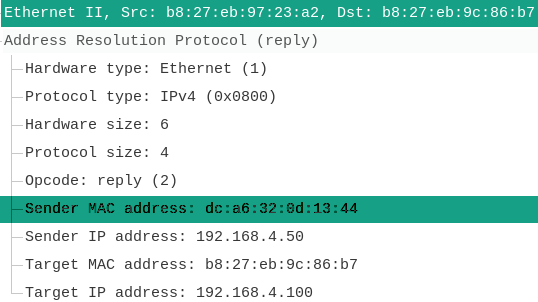
\includegraphics[scale=0.5]{../tests/RTT/proxy.png}
	\caption{Exp 2: Wireshark Proxy ARP}
	\label{fig:wireflowProxy}
\end{figure}

The mixed source MAC addresses create a distinctive ARP reply which the IDPS
can create and insert flow rule specifically tailored to.
The unique flow rule is strict in the ARP packets it forwards, preventing the adversaries MAC addresses from attempting 
any other ARP poisoning methods.
This is possible due to the flow rule matching capabilities of OpenFlow 1.3, which offers the ability to match Link-Layer
protocols such as ARP.

The code Snippet \ref{lst:proxyflowrule} below is an example of the flow rule, which has
a higher priority ensuring the switch attempts to match it before other ARP flow rules.
In the example flow rule is tailored for the ARP proxy based on the
the block MAC address \emph{b8:27:eb:9c:86:b7} with the IP \emph{192.168.4.106}; the IDPS MAC address seen as \emph{dc:a6:32:0d:13:44}.

\begin{lstlisting}[language=Bash,caption={Proxy ARP reply Flow Rule for blocked MAC},captionpos=b,label={lst:proxyflowrule}]
	priority=10,arp,dl_src=b8:27:eb:9c:86:b7,arp_spa=192.168.4.100,arp_sha=dc:a6:32:0d:13:44 actions=NORMAL
\end{lstlisting}

The ARP proxy relies on the \emph{Flow-Removed} event trigger, generated when the flow rule that is blocking ARP packets from the 
blocked MAC address \emph{idle\_timeout}, which is discussed in Section \ref{subsubsec:posarp}.
This event informs the IDPS that a MAC address is no longer actively blocked, and subsequently that the two flow rules
need to be deleted. The flow rules being the ARP request packet for the blocked MAC's IP address that is forwarded to the controller rule in Snippet \ref{lst:blockedflowrules},
as well as, the ARP proxy reply flow rule designed for the ARP proxy to reply to requests from the block MAC addresses in Snippet \ref{lst:proxyflowrule}. 

\subsection{Logging}
\label{subsec:logging}
The IDPS provides live on-screen logging of events such as DHCP offers, ARP packets and ARP poisoning, while also 
providing file logging for ARP poisoning detections. These logs are generated and managed by a newly created mechanism inside the 
class \lstinline{csvLogger} generating one file per day. The separation
in events and ARP poisoning prevents an attack being lost in the logs. The log file is stored in the CSV format which allows
the log to be directly imported to several tools that support the CSV format, such as spreadsheets. The log format is explained
below in Table \ref{table:logfile}.

\begin{table}[H]
	\centering
	\begin{tabular}{|
		>{\columncolor[HTML]{C0C0C0}}l |l|}
		\hline
		\textbf{Name}                                                            & \cellcolor[HTML]{C0C0C0}\textbf{Information}                                                                                                                                         \\ \hline
		\textbf{Date/Time}                                                       & \begin{tabular}[c]{@{}l@{}}The Date and Time the incident occurred,\\ using the format: \\ YYYY-MM-DD HH/MM/SS/USEC(6 places)\end{tabular}                                             \\ \hline
		\textbf{\begin{tabular}[c]{@{}l@{}}ARP poisoning\\ ID\end{tabular}}      & \begin{tabular}[c]{@{}l@{}}The ARP poisoning ID is to define what type of\\ ARP poisoning was detected.\\ The ID is the same format as seen in\\ requirements Table \ref{table:reqARPpos}.\end{tabular} \\ \hline
		\textbf{\begin{tabular}[c]{@{}l@{}}Offending\\ MAC Address\end{tabular}} & \begin{tabular}[c]{@{}l@{}}The MAC address that is attached to the malicious\\ ARP packet.\end{tabular}                                                                               \\ \hline
		\textbf{Packet}                                                          & \begin{tabular}[c]{@{}l@{}}The offending ARP packet as seen by the IDPS\\ and Ryu controller. This contains, Ethernet frame\\ fields and ARP frame fields.\end{tabular}              \\ \hline
		\textbf{Action Taken}                                                    & \begin{tabular}[c]{@{}l@{}}The action taken by the IDPS on detection\\ of the ARP poisoning, likely MAC blocking\end{tabular}                                                         \\ \hline
	\end{tabular}
	\caption{IDPS Log file format}
	\label{table:logfile}
\end{table}

An example of the logging CSV file is seen below in Snippet \ref{lst:idpslog}. The log shows ARP poisoning ID \emph{1.3},
ARP impersonation verified by observing the packet showing the difference in MAC source address between the Ethernet frame and ARP
headers. This attempt led to the MAC \emph{b8:27:eb:9c:86:b7} being temporarily blocked.

\begin{lstlisting}[language=Bash,caption={IDPS log example},captionpos=b,label={lst:idpslog}]
2020-08-16 02:44:12.937436,1.3,b8:27:eb:9c:86:b7,"ethernet(dst='ff:ff:ff:ff:ff:ff',ethertype=2054,src='b8:27:eb:9c:86:b7'), arp(dst_ip='192.168.4.178',dst_mac='ff:ff:ff:ff:ff:ff',hlen=6,hwtype=1,opcode=1,plen=4,proto=2048,src_ip='192.168.4.1',src_mac='b8:27:eb:97:23:a2')", MAC block 300s
\end{lstlisting}

\section{File Structure}
The entire IDPS functions primarily within a single directory, except logs which are stored within its directory.
The IDPS itself is stored within a single Python3 script, called upon using the Ryu controller to run alongside as an 
extension. Below is a summary of the files in the folder structure.
\begin{itemize}
	\itemsep0em
	\item \textbf{ARP\_IDPS.py} The IDPS Python3 code, Code in Appendix \ref{app:IDPScode}.
	\item \textbf{ARP\_IDPS\_tool.py} A simple tool to easily List, Add and Delete values in the two CSV files, Code in Appendix \ref{app:IDPStool}.
	\item \textbf{mac\_knownlist.csv} The local \emph{mac\_knownlist} file, duplicated from the IDPS file, an example in Appendix \ref{app:knownlist}.
	\item \textbf{dhcp\_whitelist.csv} The local \emph{dhcp\_whitelist} file, an example in Appendix \ref{app:whitelist}.
	\item \textbf{logs/log\_XXXXXXXX.csv} An example log file in the Logs directory, the log file contains a date stamp in the format YYYYMMDD, an example in Appendix \ref{app:idpslog}.
\end{itemize}

\section{Algorithm Overview}
The two algorithms below give an overview of the operation of the IDPS in pseudo-code, it's split between
the two core events triggered in the IDPS, the \emph{Flow-Removed} seen in algorithm \ref{fig:IDPSPsuedoCodeFlow}
and \emph{PacketIn} seen in algorithm \ref{fig:IDPSPsuedoCodePacket}.

\begin{figure}[H]
	\begin{algorithm}[H]
		\SetAlgoLined
		\DontPrintSemicolon
		\KwRequire{FlowRemoval OpenFlow Event}
		Proxy\_list = ()\\
		\SetKwProg{Def}{Function}{:}{end}
		\Def{FlowRemoval(flw: flow rule)}{
			\uIf{flow \DataSty{is in} Proxy\_list}{
				\KwSty{Delete Block Flow rule} flw.eth.src.MAC \\
				\KwSty{Delete Proxy Flow rules} flw.eth.src.MAC \\
				Proxy\_list \KwSty{remove} flw.eth.src.MAC
			}
		}
	\caption{IDPS FlowRemoval Event Algorithm}
	\end{algorithm}

	\caption{IDPS FlowRemoval Event Algorithm}
	\label{fig:IDPSPsuedoCodeFlow}
\end{figure}


\begin{figure}[H]
	\begin{algorithm}[H]
		\SetAlgoLined
		\DontPrintSemicolon
		\KwRequire{PacketIn OpenFlow Event}
		mac\_knownlist = mac\_knownlist.csv\\
		dhcp\_whitelist = dhcp\_whitelist.csv\\
		Proxy\_list = ()\\

		\SetKwProg{Def}{Function}{:}{end}
		\Def{PacketIn(pkt: packet)}{
			\uIf{pkt == DHCP}{
				\uIf{DHCP.offer.src.mac \DataSty{is in} dhcp\_whitelist}{
					mac\_knownlist \KwSty{add} DHCP.offer.pair
				}
				\uElse{
					\KwSty{Block Flow rule} DHCP.offer.src.mac \\
					\KwSty{Proxy Flow rules} DHCP.offer.src.mac \\
					Proxy\_list \KwSty{add} DHCP.offer.src.mac
				}
			}
			\uElseIf{pkt == ARP Req \KwSty{and} pkt.arp.dst.ip \DataSty{is in} Proxy\_list}{
				\KwSty{Drop} ARP.request \\
				\KwSty{ARP reply to} ARP.eth.src.mac \KwSty{from} Proxy\_list.mac
			}
			\uElseIf{pkt == ARP \KwSty{and} (pkt.eth.src.mac \KwSty{and} pkt.arp.src.ip) \DataSty{not in} mac\_knownlist}{
				mac\_knownlist \KwSty{add} ARP.pair
			}


			\uElseIf{pkt == ARP}{
				\uIf{(ARP.eth.src.mac \KwSty{and} ARP.arp.src.ip) !=  mac\_knownlist.pair}{
					\KwSty{Set} ARP.attack = \KwSty{True}
				}
				\uElseIf{(ARP.eth.dst.mac \KwSty{and} ARP.arp.dst.ip) !=  mac\_knownlist.pair}{
					\KwSty{Set} ARP.attack = \KwSty{True}
				}
				\uElseIf{ARP.eth.src.mac \DataSty{not in} mac\_knownlist \KwSty{and} ARP.arp.src.ip \DataSty{is in} mac\_knownlist}{
					\KwSty{Set} ARP.attack = \KwSty{True}
				}
				\uElseIf{ARP.eth.src.mac != ARP.arp.src.mac}{
					\KwSty{Set} ARP.attack = \KwSty{True}
				}
				\uElseIf{ARP.eth.dst.mac != ARP.arp.dst.mac}{
					\KwSty{Set} ARP.attack = \KwSty{True}
				}
				\uElseIf{ARP.opcode == Reply \KwSty{and} ARP.eth.dst.mac == "FF:FF:FF:FF:FF:FF"}{
					\KwSty{Set} ARP.attack = \KwSty{True}
				}


				\uIf{ARP.attack == \KwSty{True}}{
					\KwSty{Block Flow rule} ARP.eth.src.mac \\
					\KwSty{Proxy Flow rules} ARP.eth.src.mac \\
					Proxy\_list \KwSty{Add} ARP.eth.src.mac \\
					\KwSty{Log} ARP poisoning \KwSty{by} ARP.eth.src.mac
				}
				\uElse{
					\KwSty{Add Flow rule} ARP.eth.src.mac \KwSty{to} ARP.eth.dst.mac  \\
					\KwSty{Forward} ARP packet \\
				}
			}
		}
	\caption{IDPS PacketIn Event Algorithm}
	\end{algorithm}

	\caption{IDPS PacketIn Event Algorithm}
	\label{fig:IDPSPsuedoCodePacket}
\end{figure}


% % % % % % % % % % % % % % % % % % % % % % % % % % % % % % % % % % % % % % % % % % % % % % % % % % % % % % % %
% % % % % % % % % % % % % % % % % % % % % % % % % % % % % % % % % % % % % % % % % % % % % % % % % % % % % % % %
% % % % % % % % % % % % % % % % % % % % % % % % % % % % % % % % % % % % % % % % % % % % % % % % % % % % % % % %
% % % % % % % % % % % % % % % % % % % % % % % % % % % % % % % % % % % % % % % % % % % % % % % % % % % % % % % %
% % % % % % % % % % % % % % % % % % % % % % % % % % % % % % % % % % % % % % % % % % % % % % % % % % % % % % % %


\chapter{Testbed Implementation}
\label{Chap:testbed}
To evaluate the performance of the proposed IDPS, a physical testbed was been implemented. This chapter covers the SDN
testbed network architecture and topology, components and networking tools used as part of the testbed and as part 
of the testing.

\section{Components}
The testbed consists of a TP-Link Archer AC1750 router using OpenWRT firmware installed Open vSwitch with OpenFlow 1.3 and
dnsmasq service acting as DHCP server, RaspberryPi 4 as the SDN controller and IDPS and finally two RaspberryPi 3's
acting as a Benign host and Attacker. This section covers, in more detail, the network
components, their setup, services and software.

\subsection{TP-Link Archer AC1750 C7}
The TP-Link Archer AC1750 C7 router is an off-the-shelf router, the vendor firmware supplied by TP-link does 
not support OpenFlow or SDN features. Therefore, the open-source firmware OpenWRT
Section \ref{sec:OpenWRT} was installed onto the router. The Archer router was chosen as it is extensively supported by OpenWRT,
with detailed instructions within their documentation\cite{openwrtprojectRouter}.

\subsubsection{OpenWRT Configuration}
The Figure \ref{fig:routerdef} is provided by OpenWRT, consisting of the default inner structure
of the network.

\begin{figure}[H]
	\centering
	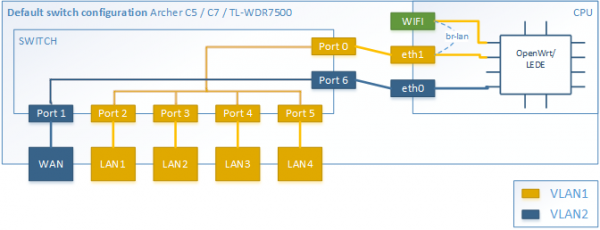
\includegraphics[scale=0.65]{images/routerinside.png}
	\caption{Default Router internal configuration \cite{openwrtprojectRouter}.}
	\label{fig:routerdef}
\end{figure}

The router consists of two core components, switch and CPU. When devices are connected to \emph{Port 2} and \emph{Port 3}
they can communicate through the switch without any traffic being seen within the CPU. As traffic passed through the switch
is not visible to the CPU, the OpenFlow switch running within the router cannot monitor any traffic,
preventing the SDN switch inside the router from being able to control the flow of traffic.


\subsubsection{SDN Configuration}
Figure \ref{fig:routerVLAN} shows the implemented SDN configuration for OpenWRT on the Archer router.
The switch is bypassed and forces traffic to flow through the CPU. This is achieved by each physical port on the switch 
being allocated its static VLAN, with each device on a separate VLAN they are unable to directly 
communicate with each other. These VLAN's provide each physical port on the router as a virtual 
interface connected to \emph{eth1}, this common interface within the CPU allows the different VLANs to send traffic between each other
while also having traffic visible within the CPU and the OvS switch.
The configuration file \lstinline{/etc/config/network} seen in Appendix \ref{app:NetworkIF}, is the interface
configuration file for OpenWRT and implements this inner network structure.

\begin{figure}[H]
	\centering
	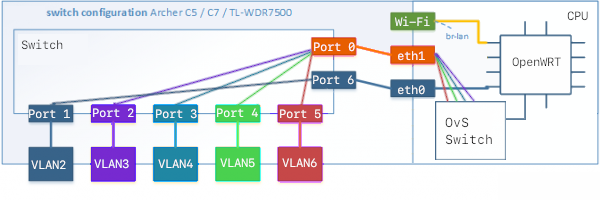
\includegraphics[scale=0.65]{images/routerinsideSDN.png}
	\caption{SDN switch internal configuration}
	\label{fig:routerVLAN}
\end{figure}

\subsubsection{Open vSwitch}
The OpenWRT firmware does not directly support SDN within its configuration. However, the package manager
(\emph{OPKG}) contains the Open vSwitch package for installation seen in Section \ref{sec:OpenWRT}, which
is then configured via the terminal. The package can be installed in the OpenWRT terminal using the
commands in Snippet \ref{lst:ovsinstall}.

\begin{lstlisting}[language=Bash,caption={OvS installation},captionpos=b,label={lst:ovsinstall}]
$ opkg update && opkg install openvswitch
\end{lstlisting}

The package comes with the \emph{ovs-vsctl} tool which is used to create an OvS bridge
with SDN switch capabilities. The Snippet \ref{lst:ovssetup} is the command used to create the \emph{br-ovs} bridge
with the OpenFlow 1.3 protocol, the IP address of the Ryu controller, the virtual interfaces and setting \lstinline{set-fail-mode}
state set as \emph{Standalone},
setting the forwarding control as a traditional switch when failing to connect to the SDN controller.
The second command sets the bridge the IP address \emph{192.168.4.1}, that's used as a gateway and the DHCP server IP address.

\lstinputlisting[language=Bash,caption={OvS setup commands},captionpos=b,label={lst:ovssetup}]
{../code/snippets/OVSwitchCMD.txt}

The SDN switch can be verified by using the \lstinline{ovs-vsctl show} command, which also indicates
if the Ryu controller has connected to the switch.
\begin{lstlisting}[language=Bash,caption={OvS Verification},captionpos=b,label={lst:ovsinstalled}]
root@OpenWrt:~$ ovs-vsctl show
b29855e0-97a9-482d-a7a0-1436473f395a
    Bridge br-ovs
				Controller "tcp:192.168.4.2:6633"
					is_connected: true
        fail_mode: standalone
        Port "eth1.6"
            Interface "eth1.6"
        Port "eth1.4"
            Interface "eth1.4"
        Port "eth1.3"
            Interface "eth1.3"
        Port "eth1.5"
            Interface "eth1.5"
        Port br-ovs
            Interface br-ovs
                type: internal
    ovs_version: "2.11.3
	\end{lstlisting}

\subsubsection{dnsmasq DHCP server}
The OpenWRT firmware uses the tool \emph{dnsmasq}\cite{kelley} as it's DHCP and DNS server, the testbed utilises
this service to configure a DHCP server on the OvS bridge and SDN network;
which the IDPS monitors to determine hosts on the network.
This is done simply by updating the configuration file stored in \lstinline{/etc/dnsmasq.conf}, seen below in Snippet \ref{lst:dnsmasq},
to offer IP addresses within the SDN
subnet \emph{192.168.4.0/24}, the configuration file allows setting static DHCP hosts and IP addresses for the devices;
such the DHCP reserving and offering the Ryu controller \emph{192.168.4.2}.

\lstinputlisting[language=Bash,caption={OpenWRT dnsmasq config file},captionpos=b,label={lst:dnsmasq}]
{../code/snippets/Archerdnsmasq.txt}


\subsection{Pi4 SDN Controller}
A RaspberryPi 4 B is utilised as the SDN controller, specifications of which are ARM Quad-core Cortex-A72, 2GB RAM
and 1GB NIC card,
using the latest version of Raspbian codename \emph{Buster}; a Debian based OS for the RaspberryPi single-board computer\cite{raspberrypi4}.
This device is connected directly to the TP-Link Archer router on VLAN 3 on the first SDN switch interface.


\subsubsection{Ryu setup}
The Ryu controller was choosen due to being Python3 based, easily installed and runs on an ARM-based chip,
while supporting OpenFlow up to 1.5.
Ryu is not available as a packaged installation in Raspbian, however, is 
open source and relies on GitHub as it's versioning repository.
To download Ryu, the following command is seen in Snippet \ref{lst:ryuinstall}:

\begin{lstlisting}[language=Bash,caption={Ryu Installation},captionpos=b,label={lst:ryuinstall}]
$ git clone https://github.com/faucetsdn/ryu .
$ pip install .
\end{lstlisting}

Executing the Ryu controller with a specified component, such as the proposed IDPS, is achieved by simply calling the Ryu 
manager and the Python3 script containing the IDPS as seen in Snippet \ref{lst:ryurun}:
\begin{lstlisting}[language=Bash,caption={Ryu Execution},captionpos=b,label={lst:ryurun}]
$ sudo ryu-manager ./ARP_IDPS.py
\end{lstlisting}


\subsection{Pi3 Hosts}
The testbed consists of two RaspberryPi 3 B+ devices, the specification being ARM Cortex-A53, 1GB Ram
with a 1GB NIC over USB 2.0 \cite{raspberrypi3}, running the latest version of Raspbian. As these two devices
are the same specification the testbed offers a more balanced testing platform. Similar to the Pi4 the
benign host \emph{phy-host-one} and attacker host \emph{phy-host-two} are 
connected on the TP-Link Archer router via VLAN's, 4 and 6 respectively.

\subsubsection{ARP Poisoning Configuration}
Configuration on the network interface is required on the attacking host to sniff packets and perform ARP Poisoning attacks.
Specifically, the networking interface needs to be configured into promiscuous mode.
Promiscuous mode opens the interface to forward all network traffic it receives to the CPU rather than
passing only the Ethernet Frames that the host is destined to receive. 
Enabling promiscuous mode is done through the \emph{Iproute2} tool as seen in Snippet \ref{lst:prommode}:
\begin{lstlisting}[language=Bash,caption={Enable Promiscuous Mode},captionpos=b,label={lst:prommode}]
ip link set eth0 promisc on
\end{lstlisting}


\newpage
\subsection{Network Time Protocol}
The Raspberry Pi's within the testbed are required to have the same internal time, as part of testing requires noting the time 
taken for packets to travel across the network in milliseconds. Raspberry Pi's do not contain a real-time clock onboard, therefore,
the time on each Pi can drift. To ensure valid results during testing the testbed uses
the Network Time Protocol (\emph{NTP}), the standard networking protocol for clock synchronization between
devices. NTP can achieve better than one-millisecond accuracy in small local LAN's,
which the testbed meets the criteria for, resulting in the Pi's having accurate \emph{Stratum 2} time.
The RaspberryPi4 and controller is set as an NTP server and the two RaspberryPi3's
are NTP clients, meaning the two RaspberryPi3's get the time from the controller; ensuring devices are configured
with the same time, as seen in Snippet \ref{lst:ntpsync}.
The configurations used for both are available in Appendix \ref{app:ntpclie} and \ref{app:ntpserv}. 
\begin{lstlisting}[language=Bash,caption={NTP Sync to Controller},captionpos=b,label={lst:ntpsync}]
pi@phy-host-one:~ $ ntpq -pn
     remote       st t when poll reach   delay   offset
=========================================================
*192.168.4.2       2 u  513  512  377    1.077    0.151
\end{lstlisting}

\subsection{Network Summary}
Table \ref{table:testbedcomp} summarises the devices connected to the Testbed and their respective interfaces, IP addresses
and MAC addresses.

\begin{table}[H]
	\centering
	\begin{tabular}{|l|l|l|l|l|}
		\hline
		\rowcolor[HTML]{C0C0C0} 
		\textbf{Device}                                                   & \textbf{\begin{tabular}[c]{@{}l@{}}Device\\ Hostname\end{tabular}} & \textbf{\begin{tabular}[c]{@{}l@{}}Network\\ Interface\end{tabular}} & \textbf{IP address} & \textbf{MAC Address} \\ \hline
		\textbf{\begin{tabular}[c]{@{}l@{}}Open\\ vSwitch\end{tabular}}   & openwrt                                                            & br-ovs                                                               & 192.168.4.1         & 00:00:aa:bb:cc:dd    \\ \hline
		\textbf{\begin{tabular}[c]{@{}l@{}}Ryu\\ Controller\end{tabular}} & phy-ryu                                                            & eth1.3                                                               & 192.168.4.2         & dc:a6:32:0d:13:44    \\ \hline
		\textbf{\begin{tabular}[c]{@{}l@{}}Benign\\ Host\end{tabular}}    & phy-host-one                                                       & eth1.4                                                               & 192.168.4.50        & b8:27:eb:97:23:a2    \\ \hline
		\textbf{Attacker}                                                 & phy-host-two                                                       & eth1.6                                                               & 192.168.4.100       & b8:27:eb:9c:86:b7    \\ \hline
	\end{tabular}
	\caption{Testbed Hosts network Configurations}
	\label{table:testbedcomp}
\end{table}

\subsection{Network Architecture}
The network devices are connected in a star network topology, whereby every device is connected with the TP-Link Archer AC1750
acting as the central hub containing the SDN switch. The implementation is the simplest network form and forces all traffic 
in the network to pass through the SDN OvS switch. Figure \ref{fig:testbednet} below shows the testbed environment, including
the services they provide, while Figure \ref{fig:physicalTestbed} is a picture of the physical testbed.

\begin{figure}[H]
	\centering
	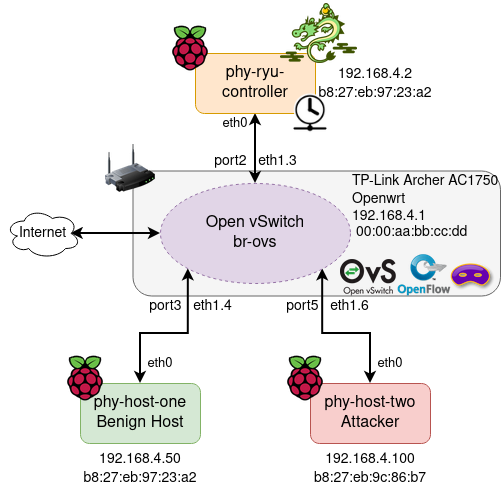
\includegraphics[scale=0.65]{images/networktopo.png}
	\caption{Testbed Network Topology}
	\label{fig:testbednet}
\end{figure}

\begin{figure}[H]
	\centering
	\includegraphics[scale=0.73]{images/testbedReal.png}
	\caption{SDN switch internal configuration}
	\label{fig:physicalTestbed}
\end{figure}

\section{Custom Tools}
As part of testing and development two custom tools were specificaly created,
this section briefly covers their purpose, functionality and implementation.

\subsection{IDPS Configuration Tool}
\label{subsec:idpsconfig}off
An external command-line interface tool called \emph{ARP\_IDPS\_tool} was created to offer user 
configuration of the CSV files the IDPS
relies upon, such as \emph{mac\_knownlist} and \emph{dhcp\_whitelist}. This allows users to add Static IP addresses
and MAC address pairings to the \emph{mac\_knownlist}, or adding or deleting DHCP servers from the \emph{dhcp\_whitelist}.
This tool is a simple Python3 script 
which incocprates the \lstinline{csvMACListTracker} class, the Snippet \ref{lst:arptool} is the help menu 
from the tool which is available in the Appendix \ref{app:IDPStool}.

\begin{lstlisting}[language=Bash,caption={ARP\_IDPS\_Tool Help Menu},captionpos=b,label={lst:arptool}]
pi@phy-ryucontroller-01:~ $ ./ARP_IDPS_tool.py -h
usage: [-h] [-l] [-a ADD] [-d DELETE] [-f] file

Simple tool to Manage ARP IDPS CSV files

positional arguments:
  file        CSV file to use

optional arguments:
  -h, --help  show this help message and exit
  -l          List CSV file
  -a ADD      Add Mac to CSV
  -d DELETE   Delete row Containg MAC to CSV
  -f          Flush entire CSV file
\end{lstlisting}

\subsection{IDPS Testing Tool}
\label{subsec:testingtool}
As the proposed system was developed to meet a set of criteria (\emph{Table \ref{table:reqARPpos}}) for detecting ARP Poisoning,
a tool is required to generate the specific ARP poisoning packets. To avoid using a variety of tools that implement these 
attacks in their versions, resulting in different packets and timings, a custom tool was specifically developed.
Additionally, there is the option of measuring CPU load, required when measuring the proposed system on the controller. 
The tool 
is called \emph{ARP\_IDPS\_test} and ran via the command line, the source code can be seen in Appendix \ref{app:IDPStestcode}.
The tool uses simple command-line options to determine what ARP poisoning packets or test to perform and the parameters the test should use,
such as how many times to perform the action and the frequency.

\subsubsection{ARP Request \& Reply}
The tool generates standard and poisoned ARP packets for testing the proposed IDPS effectiveness,
relying on the Python3 \emph{scapy} library to create and send the individual ARP packets. The library
offers a simple function to create packets as seen in Snippet \ref{lst:scapyarp}, with arguments to insert any 
combination of MAC and IP pairings in Ethernet Frame and ARP Headers.

\begin{lstlisting}[language=Bash,caption={Scapy ARP packet creation},captionpos=b,label={lst:scapyarp}]
scapy.Ether(dst=DSTMAC, src=SRCMAC) / scapy.ARP(op="who-has", hwsrc=SRCMAC, psrc=SRCIP, hwdst=DSTMAC, pdst=DSTIP)
\end{lstlisting}

This flexibility offered by \emph{scapy} allows the generation of ARP packets meeting the proposed IDPS criteria, such as
the mismatch of source MAC address in the Ethernet Frame and ARP Header (\emph{A2.3}).

\subsubsection{CPU Testing}
The CPU load function is achieved using the Python library \emph{PSutil} as discussed in Section \ref{subsec:Scapy}.
The library offers many resource system monitoring options, however, the tool relies on the library for measuring
the total CPU load consistently over an extended period. This is achieved by measuring each CPU core activity
and dividing it by the total core's to calculate the average load.

\subsubsection{Log File's}
Each test performed by the tool produces a CSV log file similar to
the proposed IDPS logging as described in Section \ref{subsec:logging}. The CSV format ensures the logs can be easily 
imported into spreadsheet software and easily comparable against the IDPS log, the tool in Appendix \ref{app:timediffcode}
is one such tool used to calculate the time difference between the logs for RTT testing.

Table \ref{table:idpstoolog} and Snippet \ref{lst:a11log} are an example log used for testing an ARP request 
Poisoning criteria.
\begin{table}[H]
	\centering
	\begin{tabular}{|
		>{\columncolor[HTML]{9B9B9B}}l |c|}
		\hline
		\multicolumn{1}{|c|}{\cellcolor[HTML]{9B9B9B}\textbf{Name}} & \cellcolor[HTML]{9B9B9B}\textbf{Information}                                                           \\ \hline
		\textbf{Packet \#}                                          & Packet Number                                                                                         \\ \hline
		\textbf{Date/Time}                                          & \begin{tabular}[c]{@{}c@{}}The Date and Time when a\\ packet was sent, down to microseconds\end{tabular} \\ \hline
		\textbf{Response}                                           & \multicolumn{1}{l|}{If the ARP request had a reply}                                                    \\ \hline
		\end{tabular}
		\caption{IDPS tool log example}
		\label{table:idpstoolog}
\end{table}
\begin{lstlisting}[language=Bash,caption={Test tool log Example},captionpos=b,label={lst:a11log}]
0,2020-08-24 16:41:59.314034,0
\end{lstlisting}

\subsubsection{Example Usage}
The Snippet \ref{lst:a11att} is an example of using the testing tool from the Attacker host, the tool 
performs an ARP poison using the \emph{A1.1} criteria, attempting the ARP every ten seconds twenty five times.
The full help menu can be seen in Appendix \ref{app:testcodehelp}
\begin{lstlisting}[language=Bash,caption={ARP Poison test tool Usage},captionpos=b,label={lst:a11att}]
	sudo ./ARP_IDPS_test.py -p 1.1 -c 25 -t 10
\end{lstlisting}

% % % % % % % % % % % % % % % % % % % % % % % % % % % % % % % % % % % % % % % % % % % % % % % % % % % % % % % %
% % % % % % % % % % % % % % % % % % % % % % % % % % % % % % % % % % % % % % % % % % % % % % % % % % % % % % % %
% % % % % % % % % % % % % % % % % % % % % % % % % % % % % % % % % % % % % % % % % % % % % % % % % % % % % % % %
% % % % % % % % % % % % % % % % % % % % % % % % % % % % % % % % % % % % % % % % % % % % % % % % % % % % % % % %
% % % % % % % % % % % % % % % % % % % % % % % % % % % % % % % % % % % % % % % % % % % % % % % % % % % % % % % %

\chapter{Experiments and Results}
A total of three experiments were performed on the proposed and implemented IDPS discussed in Chapter \ref{Chap:DesImp},
the IDPS code is available within Appendix \ref{app:IDPScode}.
The experiments consisted of testing the IDPS at detecting a variety of poisoned ARP packets, 
the impact the proposed IDPS has on ARP traffic RTT and the overhead imposed on the controller.
Each experiment was performed on the physical testbed see Chapter \ref{Chap:testbed}, any alterations to the testbed
setup is explicitly stated within the experiment itself.

\section{Experiment Limitations}
The experiments used the specifically created testing tool from Section \ref{subsec:testingtool} to gather results.
The tool relies on the Python3 \emph{Scapy} library to send and receive packets, the library introduces a delay
in packet speed as it pulls Link-Layer ARP packets out to the application and vice versa. This delay is
noticeably visible when comparing RTT of ARP packets using the \emph{arping} tool and \emph{scapy} library,
as seen in Table \ref{table:scapydelay} which contains the average RTT of an ARP request.

\begin{table}[H]
	\centering
	\begin{tabular}{|
		>{\columncolor[HTML]{9B9B9B}}l |c|c|c|c|}
		\hline
		\multicolumn{1}{|c|}{\cellcolor[HTML]{9B9B9B}\textbf{Tool}} & \cellcolor[HTML]{9B9B9B}\textbf{ARP 1} & \cellcolor[HTML]{9B9B9B}\textbf{ARP 2} & \cellcolor[HTML]{9B9B9B}\textbf{ARP 3} & \cellcolor[HTML]{9B9B9B}\textbf{Average} \\ \hline
		\textbf{arping}                                             & 579.1usec                              & 582.0usec                              & 609.1usec                              & 0.59ms                                   \\ \hline
		\textbf{scapy}                                              & 42.2ms                                 & 42.1ms                                 & 42.0ms                                 & 42.1ms                                   \\ \hline
		\end{tabular}
	\caption{arping And Scapy ARP RTT Limitaition}
	\label{table:scapydelay}
\end{table}

Therefore, all testing relies on the \emph{scapy} library to maintain a consistent testing environment, this includes normal
ARP packets and poisoned ARP packets. The only exception being the Ryu Controller which receives packets via the
OpenFlow \emph{PacketIn} event.

% % % % % % % % % % % % % % % % % % % % % % % % % % % % % % % % % % % % % % % % % % % % % % % % % % % % % % % %
\newpage
\section{Experiment 1: Variety of Poisoning Detection and Mitigation}
\begin{minipage}{0.48\textwidth}
		
	The first experiment aimed to verify the proposed IDPS core operation. The experiment
	was performed to determine that the proposed IDPS met the objective of detecting and mitigating poisoned ARP packets, regardless of specific
	metrics such as RTT and CPU usage.
	This experiment uses the earlier defined ARP poisoning criteria Table \ref{table:reqARPpos} also seen below in
	Table \ref{table:arpdetcrit}, to perform a variety of ARP poisoning attacks conducted against the Benign host from the Attacker host.
	To determine how accurate the proposed system is at detecting and mitigating the poisoned ARP packets, and 
	how quickly there detected.
	

\end{minipage} \hfill
\begin{minipage}{0.50\textwidth}
	\begin{table}[H]
		\centering
		\begin{tabular}{|
			>{\columncolor[HTML]{C0C0C0}}l |l|}
			\hline
			\textbf{ID}                         & \cellcolor[HTML]{C0C0C0}\textbf{Attack}                            \\ \hline
			\cellcolor[HTML]{FE996B}\textbf{A1} & \cellcolor[HTML]{FE996B}ARP Request                                \\ \hline
			\textbf{A1.1}                       & ARP IP known spoof                                                 \\ \hline
			\textbf{A1.2}                       & \begin{tabular}[c]{@{}l@{}}ARP IP unknown\\ spoof\end{tabular}     \\ \hline
			\textbf{A1.3}                       & Source MAC mismatch                                                \\ \hline
			\cellcolor[HTML]{68CBD0}\textbf{A2} & \cellcolor[HTML]{68CBD0}ARP Reply                                  \\ \hline
			\textbf{A2.1}                       & ARP IP SRC spoof                                                   \\ \hline
			\textbf{A2.2}                       & ARP IP DST spoof                                                   \\ \hline
			\textbf{A2.3}                       & Source MAC mismatch                                                \\ \hline
			\textbf{A2.4}                       & \begin{tabular}[c]{@{}l@{}}Destination MAC\\ mismatch\end{tabular} \\ \hline
			\textbf{A2.5}                       & Destination masked                                                 \\ \hline
			\end{tabular}
		\caption{IDPS ARP detection Criteria}
		\label{table:arpdetcrit}
	\end{table}
\end{minipage}

\subsection{Experiment Setup}
The tests in this experiment use the MAC address and IP address pairing in the \emph{mac\_knownlist} seen below
Snippet \ref{lst:macknownfile}.

\begin{lstlisting}[language=Bash,caption={Known MAC list pairing file},captionpos=b,label={lst:macknownfile}]
00:00:aa:bb:cc:dd,"{'LastIP':'192.168.4.1', 'Type':'DHCP'}"
dc:a6:32:0d:13:44,"{'LastIP':'192.168.4.2', 'Type':'DHCP'}"
b8:27:eb:97:23:a2,"{'LastIP':'192.168.4.50', 'Type':'DHCP'}"
b8:27:eb:9c:86:b7,"{'LastIP':'192.168.4.100', 'Type':'DHCP'}"
\end{lstlisting}

The ARP attacks were conducted and logged by \emph{phy-host-two} using the specifically created Python attacker
tool in Section \ref{subsec:testingtool}.
The proposed IDPS running alongside the Ryu Controller maintains it's own log file containing attemped
and prevented ARP poisoning packets.

\subsection{Measurements} 
The focus of this expierment is validation of the detection and mitigation.
Therefore, the metrics gathered for the experiment are the following:
\begin{itemize}
  \itemsep0em 
  \item \textbf{Count:} The amount of poisoned ARP packet that were detected, E.G dropped and MAC blocked by IDPS.
  \item \textbf{Time:} The IDPS detection time, which is calculated by subtracting the IDPS detection time and ARP message sent time by Attacker.
\end{itemize}

\begin{figure}[H]
  \centering
  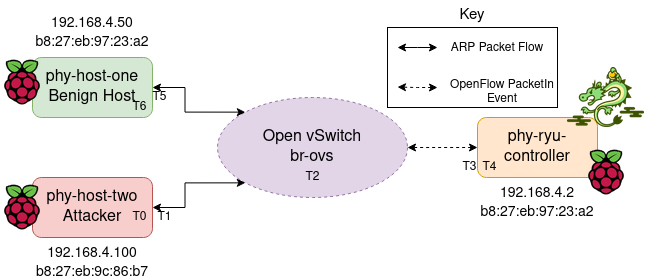
\includegraphics[scale=0.6]{images/exp1set.png}
  \caption{Exp 1: Setup and Measurement Points}
  \label{fig:exp1points}
\end{figure}

Figure \ref{fig:exp1points} shows the testbed setup containing the potential sampling points to detect ARP packets and their detection time,
seen as \textbf{T0} to \textbf{T6}. This experiment uses \textbf{T0} and \textbf{T4} sampling points to determine the packet detection \& prevention time,
these points are the testing tool sending an ARP packet and the proposed IDPS detecting and preventing the ARP packet.
The time difference seen between Attacking tool sending the packet log and the IDPS prevention log is compared to calculate
the time it took to detect the poisoned ARP.
The testing tool sends a poisoned ARP packet every \emph{10} seconds with the IDPS 
setting an \emph{idle\_timeout} on blocked MAC addresses to \emph{5} seconds, this means the flow rule actively blocking the MAC 
has been removed between packets. This is conducted fifty times to calculate the average detection and prevention time.

\subsection{Poisoned ARP Request Detection \& Mitigation}
The poisoned ARP requests packets are criteria \emph{A1.1},\emph{A1.2} and \emph{A1.3}.
These are tested by host \emph{phy-host-two} sending poisoned ARP packets to \emph{phy-host-one}, where the IDPS should detect
and block the \emph{phy-host-two} MAC address.

\subsubsection{Test A1.1 - ARP IP spoof}
Test \emph{A1.1} is the most common type of poisoned ARP, which consists of an Attacker impersonating a host to a Victim,
tested by the Attacker host sending an ARP request to the Victim with a spoofed source IP address in the ARP header.
In the test the Attacker is impersonating the gateway IP address \emph{192.168.4.1}, to
the Benign host which the IDPS knows by the \emph{mac\_knownlist} is not owned by his MAC address; as seen in Snippet \ref{lst:scapya11}.

\begin{lstlisting}[language=Bash,caption={Scapy A1.1 Test},captionpos=b,label={lst:scapya11}]
Ether(MAC_DST=FF:FF:FF:FF:FF:FF, MAC_SRC=b8:27:eb:9c:86:b7)
ARP(MAC_SRC=b8:27:eb:9c:86:b7, IP_SRC=192.168.4.1, MAC_DST=FF:FF:FF:FF:FF:FF, IP_DST=192.168.4.50)
\end{lstlisting}

\subsubsection{Test A1.2 - ARP Unknown MAC IP spoof}
Test \emph{A1.2} is the same as the prior test \emph{A1.2} except the IDPS does not know the adversaries MAC address,
therefore the MAC address is blocked but no proxy given. This test requires the use of the \emph{IDPS Config tool} discussed
in Section \ref{subsec:idpsconfig}, this is to remove the Attackers MAC address from the \emph{mac\_knownlist}.


\subsubsection{Test A1.3 - ARP Source MAC Mismatch}
The last ARP request test conducted detects and mitigates ARP IP poisoning when the 
source MAC address is mismatched. Specifically, when the Ethernet frame source MAC address differs from the 
source MAC address within the ARP payload, as seen in Snippet \ref{lst:scapya13}.
\begin{lstlisting}[language=Bash,caption={Scapy A1.3 Test},captionpos=b,label={lst:scapya13}]
Ether(MAC_DST=FF:FF:FF:FF:FF:FF, MAC_SRC=b8:27:eb:9c:86:b7)
ARP(op="who-has", MAC_SRC=b8:27:eb:9c:86:ff, IP_SRC=192.168.4.100, MAC_DST=FF:FF:FF:FF:FF:FF, IP_DST=192.168.4.50)
\end{lstlisting}


\subsection{Poisoned ARP Reply Detection \& Mitigation}
The poisoned ARP reply packets are criteria \emph{A2.1},\emph{A2.2},\emph{A2.3},\emph{A2.4} and \emph{A2.5}.
These tests differ in how they are produced, ARP reply packets are often sent as a reply to an ARP request.
However, these tests relied on the custom attacker tool instead, sending gratuitous ARP replies to \emph{phy-host-one},
whereby the receiver has not requested the ARP reply.

\subsubsection{Test A2.1 \& A2.2 - ARP IP spoof}
Testing \emph{A2.1} is similar to \emph{A1.1} however, instead of an ARP request, sending a gratuitous ARP reply. Whereby 
the IDPS detects poisoned packets if the IP address within the ARP belongs to the MAC address. Criteria \emph{A2.1} checks the
Source IP and MAC pairing as seen in Snippet \ref{lst:scapya21}.

\begin{lstlisting}[language=Bash,caption={Scapy a25.1 Test},captionpos=b,label={lst:scapya21}]
Ether(MAC_DST=b8:27:eb:97:23:a2, MAC_SRC=b8:27:eb:9c:86:b7)
ARP(op="is-at", MAC_SRC=b8:27:eb:9c:86:b7, IP_SRC=192.168.4.1, MAC_DST=b8:27:eb:97:23:a2, IP_DST=192.168.4.50)
\end{lstlisting}

Criteria \emph{A2.2} 
checks the destination IP and MAC pairing as seen in Snippet \ref{lst:scapya22}.

\begin{lstlisting}[language=Bash,caption={Scapy A2.2 Test},captionpos=b,label={lst:scapya22}]
Ether(MAC_DST=00:00:aa:bb:cc:dd MAC_SRC=b8:27:eb:9c:86:b7)
ARP(op="is-at", MAC_SRC=b8:27:eb:9c:86:b7, IP_SRC=192.168.4.100, MAC_DST=00:00:aa:bb:cc:dd, IP_DST=192.168.4.50)
\end{lstlisting}

\subsubsection{Test A2.3 \& 2.4 - ARP MAC Mismatch}
Testing criteria of \emph{A2.3} and \emph{A2.4} is a simple validation for poisoned ARPs by ensuring the MAC addresses within the
Ethernet Frame and ARP Header match. Criteria \emph{A2.3} is the source MAC addresses match, while \emph{A2.4} is the verification
of the destination MAC addresses. Shown in Snippets \ref{lst:scapya23} and \ref{lst:scapya24} respectively.

\begin{lstlisting}[language=Bash,caption={Scapy A2.3 Test},captionpos=b,label={lst:scapya23}]
Ether(MAC_DST=b8:27:eb:97:23:a2, MAC_SRC=00:00:aa:bb:cc:dd)
ARP(op="is-at", MAC_SRC=b8:27:eb:9c:86:b7, IP_SRC=192.168.4.100, MAC_DST=b8:27:eb:97:23:a2, IP_DST=192.168.4.50)
\end{lstlisting}
\begin{lstlisting}[language=Bash,caption={Scapy A2.4 Test},captionpos=b,label={lst:scapya24}]
Ether(MAC_DST=00:00:aa:bb:cc:dd) MAC_SRC=b8:27:eb:9c:86:b7)
ARP(op="is-at", MAC_SRC=b8:27:eb:9c:86:b7, IP_SRC=192.168.4.100, MAC_DST=b8:27:eb:97:23:a2, IP_DST=192.168.4.50)
\end{lstlisting}

\subsubsection{Test A2.5 - ARP Masked Destination}
The final test and criteria \emph{A2.5} is a validating the gratuitous ARP reply by MAC destination, ensuring 
the packet is addressed and not being broadcasted. Therefore, the ARP verification checks the MAC destination is not 
\emph{FF:FF:FF:FF:FF:FF}, as seen in Snippet \ref{lst:scapya25}.
\begin{lstlisting}[language=Bash,caption={Scapy A2.5 Test},captionpos=b,label={lst:scapya25}]
Ether(MAC_DST=FF:FF:FF:FF:FF:FF, MAC_SRC=b8:27:eb:9c:86:b7)
ARP(op="is-at", MAC_SRC=b8:27:eb:9c:86:b7, IP_SRC=192.168.4.100, MAC_DST=FF:FF:FF:FF:FF:FF, IP_DST=192.168.4.50)
\end{lstlisting}


\subsection{Results}
Experiment 1 results are presented in Table \ref{table:exp1res} and Figure \ref{fig:rttexpset}, which contains the ARP poison criteria tested,
attempts made, detection rate and the average time taken to detect and prevent the ARP packet. The results
indicated the proposed IDPS can accurately detect and prevent poisoned ARP packets within \emph{58.1ms}, this average
time is extremely efficient considering Table \ref{table:scapydelay} indicates an ARP RTT takes approximately \emph{42.1ms}.
The \emph{16ms} difference between a RTT ARP and detection and prevention of a poisoned ARP is a minimal time difference,
demonstrating the efficiency of the proposed IDPS.
The average detection time between ARP requests and ARP reply attacks shows no significant difference
 in detection times regardless of the type of ARP poisoning technique deployed.

Furthermore, the IDPS demonstrated an accurate assessment of ARP packets by accurately detecting every poisoned ARP packet
forwarded through the SDN network, as testing involved standard ARP packets between hosts during testing there was no 
indication of miss identification.

\begin{table}[H]
	\centering
	\begin{tabular}{|l|l|c|c|c|}
		\hline
		\rowcolor[HTML]{9B9B9B} 
		\multicolumn{1}{|c|}{\cellcolor[HTML]{9B9B9B}\textbf{ID}} & \multicolumn{1}{c|}{\cellcolor[HTML]{9B9B9B}\textbf{Attack}}         & \textbf{Attacks} & \textbf{Detected} & \textbf{\begin{tabular}[c]{@{}c@{}}Detection\\ Time Avg\end{tabular}} \\ \hline
		\rowcolor[HTML]{FE996B} 
		\textbf{A1}                                               & \multicolumn{4}{l|}{\cellcolor[HTML]{FE996B}\textbf{ARP Request}}                                                                                                               \\ \hline
		\cellcolor[HTML]{C0C0C0}\textbf{A1.1}                     & \begin{tabular}[c]{@{}l@{}}ARP IP\\ known spoof\end{tabular}         & 50               & 50                & 59.9ms                                                            \\ \hline
		\cellcolor[HTML]{C0C0C0}\textbf{A1.2}                     & \begin{tabular}[c]{@{}l@{}}ARP IP\\ unknown spoof\end{tabular}       & 50               & 50                & 57.5ms                                                            \\ \hline
		\cellcolor[HTML]{C0C0C0}\textbf{A1.3}                     & \begin{tabular}[c]{@{}l@{}}Source MAC\\ mismatch\end{tabular}        & 50               & 50                & 59.3ms                                                            \\ \hline
		\rowcolor[HTML]{68CBD0} 
		\textbf{A2}                                               & \multicolumn{4}{l|}{\cellcolor[HTML]{68CBD0}\textbf{ARP Reply}}                                                                                                                 \\ \hline
		\cellcolor[HTML]{C0C0C0}\textbf{A2.1}                     & \begin{tabular}[c]{@{}l@{}}ARP IP\\ SRC spoof\end{tabular}           & 50               & 50                & 59.3ms                                                            \\ \hline
		\cellcolor[HTML]{C0C0C0}\textbf{A2.2}                     & \begin{tabular}[c]{@{}l@{}}ARP IP\\ DST spoof\end{tabular}           & 50               & 50                & 58.1ms                                                            \\ \hline
		\cellcolor[HTML]{C0C0C0}\textbf{A2.3}                     & \begin{tabular}[c]{@{}l@{}}Source MAC\\ mismatch\end{tabular}        & 50               & 50                & 57.6ms                                                            \\ \hline
		\cellcolor[HTML]{C0C0C0}\textbf{A2.4}                     & \begin{tabular}[c]{@{}l@{}}Destination\\ MAC\\ mismatch\end{tabular} & 50               & 50                & 56.6ms                                                            \\ \hline
		\cellcolor[HTML]{C0C0C0}\textbf{A2.5}                     & \begin{tabular}[c]{@{}l@{}}Destination\\ masked\end{tabular}         & 50               & 50                & 56.4ms                                                            \\ \hline
		\rowcolor[HTML]{67FD9A} 
		\multicolumn{2}{|r|}{\cellcolor[HTML]{67FD9A}\textbf{Total/Avg}}                                                                 & \textbf{400}     & \textbf{400}      & \textbf{58.1ms}                                                   \\ \hline
		\end{tabular}
	\caption{Exp 1: Total Result's Table}
	\label{table:exp1res}
\end{table}

Figure \ref{fig:a13detected} displays the network capture during the testing of criteria \emph{A1.1},
the OpenFlow \emph{PacketIn} event
is triggered as seen by packet \emph{9} and \emph{11}, where the IDPS drops the ARP packet which cannot be seen in the monitoring as
it's never forwarded into the OvS switch.

\begin{figure}[H]
	\centering
	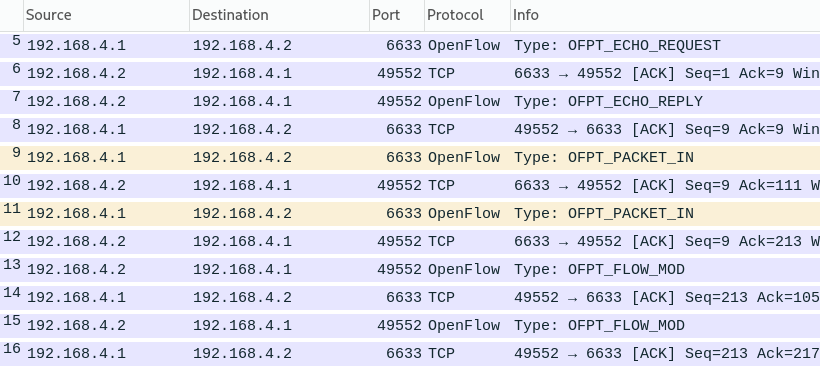
\includegraphics[scale=0.49]{../tests/a11/packetinNoArp.png}
	\caption{Exp 1: A1.1: Wireshark PacketIn Event, Blocked ARP}
	\label{fig:a13detected}
\end{figure}

\newpage
Figure \ref{fig:arpa21l} and Figure \ref{fig:a21detected} are the IDPS live log of detection and prevention during testing 
criteria \emph{A2.1}. The first figure is the IDPS indicating and logging the detection of the poisoned ARP and blocking 
further traffic, the second figure is the OpenFlow rules set within the OvS switch that are actively inserted to carry out
the IDPS MAC blocking.
\begin{figure}[H]
	\centering
	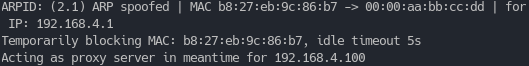
\includegraphics[scale=0.7]{../tests/a21/IDPSCap.png}
	\caption{Exp 1: ARP A2.1 IDPS Detection Log}
	\label{fig:arpa21l}
\end{figure}

\begin{figure}[H]
	\centering
	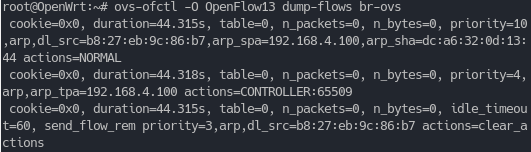
\includegraphics[scale=0.65]{../tests/a11/dumpedrules.png}
	\caption{Exp 1: A2.1: OvS OpenFlow Rules After Detection}
	\label{fig:a21detected}
\end{figure}

Figure \ref{fig:rttexpset} shows a combined plot chart containing all the results for the \emph{400} ARP packets,
including the trend line as an average. The chart shows a clear similarity in detection time and the speed in which
a malicious ARP packet is prevented. Individual results for each criteria can be seen in Appendix \ref{app:Exp1}, which contains the IDPS log for detecting the 
poisoned ARP and a plot chart containing all the results.

\begin{figure}[H]
	\centering
	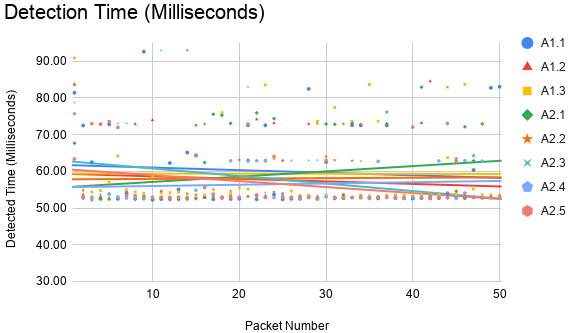
\includegraphics[scale=0.63]{images/AllARPDet.png}
	\caption{Exp 1: Summary of ARP Poisoned Detection Time (Millisecond)}
	\label{fig:rttexpset}
\end{figure}


% % % % % % % % % % % % % % % % % % % % % % % % % % % % % % % % % % % % % % % % % % % % % % % % % % % % % % % %


\newpage
\section{Experiment 2: ARP RTT Time}
As the proposed IDPS intends to have a minimal effect on the functionality and speed of ARP reply request packets,
experiment 2 measured the impact the proposed system had on the ARP round trip time (RTT). As the experiment focused on
ARP RTT time with the proposed IDPS functioning, the testbed was the same, with the exception that the attacker host was
not actively ARP poisoning; instead of using regular ARP and measuring the RTT in different scenarios.


\subsection{Experiment Setup}
The experiment uses the custom testing tool implemented in Section \ref{subsec:testingtool} on \emph{phy-host-two} host,
acting as a Benign host within this experiment. There are four different scenarios an ARP request traverses the IDPS SDN. Therefore,
the experiment is repeated in the following scenarios:

\begin{itemize}
  \itemsep0em 
  \item \textbf{Traditional Network:} A base RTT set within a traditional network using the custom tool.
          Disabling the SDN controller, enables the OvS fail mode to \emph{Standalone}; functioning as a non-SDN switch.
  \item \textbf{Existing Flow Rule:} The RTT through the proposed SDN system after the specific ARP flow rule has been installed by the IDPS.
  \item \textbf{New Flow Rule} Thee RTT of a new ARP request/reply encounter whereby the controller forwards ARP and flow rule being installed.
  \item \textbf{Proxy Server} The RTT when the proposed IDPS is acting as a proxy server and consistently replying for a blocked MAC address.
\end{itemize}


\subsection{Measurements}
\begin{figure}[H]
  \centering
  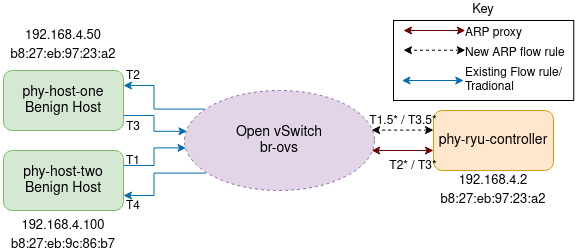
\includegraphics[scale=0.65]{../tests/RTT/diag.png}
  \caption{Exp 2: RTT Measurement Sampling Points}
  \label{fig:rttexpset}
\end{figure}

Figure \ref{fig:rttexpset} is the experiment setup and shows the time sampling points measuring the RTT. 
The RTT is the measurement of time for the responding host (\emph{phy-host-two}) to receive a response to
a ARP request. Therefore, the initial time is when the ARP request was sent from the host and the RTT is when
an ARP reply was received. In each scenario an ARP request is continuously sent every \emph{10} seconds from \emph{phy-host-two}
to \emph{phy-host-one}, this occurred for a total of fifty times.
The tool was used within \emph{phy-host-two},
therefore the sampling points used within the experiment are \textbf{T1} and \textbf{T4}, the figure also helps demonstrate the potential
routes.

\subsection{Results \& Analysis}
\label{subsec:rttres}
Table \ref{table:avgrtt} contains the average, minimum and maximum RTT for the fifty ARP reply/request tests for each four scenarios.
The bar charts in Figure \ref{fig:allarp} is the overall results for all \emph{400} ARP reply/request RTT.

\begin{table}[H]
	\centering
	\begin{tabular}{|c|c|c|c|c|}
		\hline
		\rowcolor[HTML]{9B9B9B} 
		\textbf{Scenario}                                                                             & \textbf{\begin{tabular}[c]{@{}c@{}}Average\\ RTT\end{tabular}} & \textbf{\begin{tabular}[c]{@{}c@{}}Minimum\\ RTT\end{tabular}} & \textbf{\begin{tabular}[c]{@{}c@{}}Maximum\\ RTT\end{tabular}} & \textbf{\begin{tabular}[c]{@{}c@{}}Percent\\ Increase\\ from Base\end{tabular}} \\ \hline
		\cellcolor[HTML]{C0C0C0}\textbf{Baseline}                                                     & 45.44ms                                                        & 42.02ms                                                        & 62.87ms                                                        & \cellcolor[HTML]{ECF4FF}N/A                                                     \\ \hline
		\cellcolor[HTML]{C0C0C0}\textbf{\begin{tabular}[c]{@{}c@{}}Existing\\ Flow Fule\end{tabular}} & 46.60ms                                                        & 42.04ms                                                        & 62.66ms                                                        & \cellcolor[HTML]{9AFF99}2.6\%                                                   \\ \hline
		\cellcolor[HTML]{C0C0C0}\textbf{\begin{tabular}[c]{@{}c@{}}New Flow\\ Rule\end{tabular}}      & 96.52ms                                                        & 74.5ms                                                         & 128.82ms                                                       & \cellcolor[HTML]{FFFC9E}112.5\%                                                 \\ \hline
		\cellcolor[HTML]{C0C0C0}\textbf{\begin{tabular}[c]{@{}c@{}}Proxy\\ Server\end{tabular}}       & 125.94ms                                                       & 92.9ms                                                         & 167.2ms                                                        & \cellcolor[HTML]{FFCCC9}212.5\%                                                 \\ \hline
	\end{tabular}
	\caption{Exp 2: Avg/Min/Max RTT in Each Scenario}
	\label{table:avgrtt}
\end{table}

\begin{figure}[H]
  \centering
  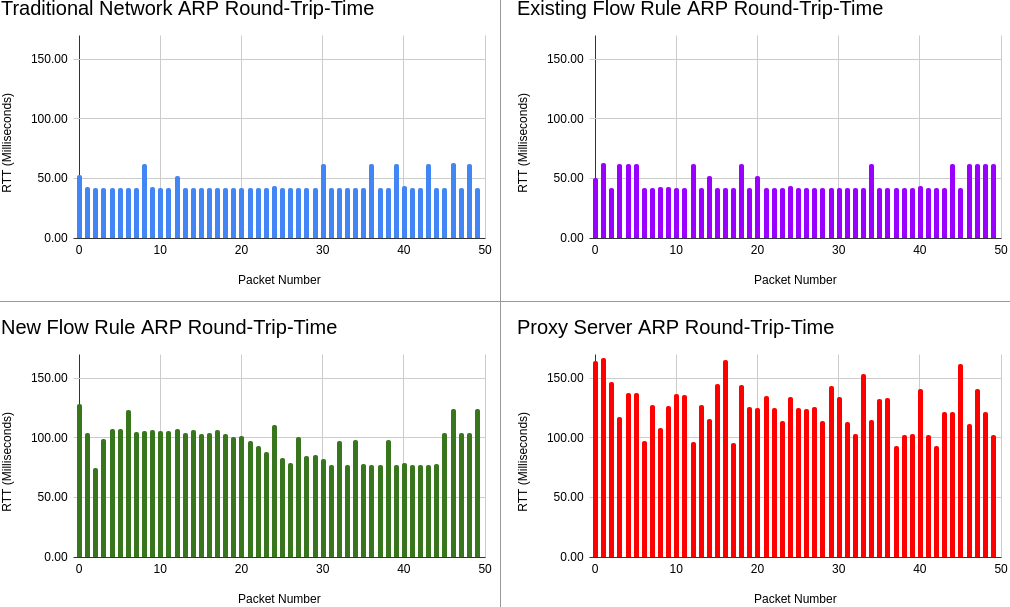
\includegraphics[scale=0.35]{../tests/RTT/allfour.png}
  \caption{Exp 2: All Four ARP Round-Trip-Time Bar Charts, Avaiable in Appendix Section \ref{app:Exp2}.}
  \label{fig:allarp}
\end{figure}

\newpage
The results suggest that the proposed system has minimal effect on the ARP RTT 
once a flow rule has been established, with the RTT \emph{45.44ms} and \emph{46.60ms} for Baseline and SDN flow rules respectively.
This is due to the proposed system actively installing specific ARP flow rules for verified packets rather then re-verifying, which 
slows down all ARP packets.

This is seen in the table \ref{table:avgrtt}, for \emph{New Flow Rule} scenario, as the ARP packet is forwarded
to the controller, the RTT has increased due to waiting for IDPS verification.
Figure \ref{fig:wireflow} is a Wireshark capture of the communication between the switch and controller where OpenFlow
sends a \emph{PacketIn} event due to the new ARP packet, and the \emph{Flow\_mod} event to install the ARP flow rule.

\begin{figure}[H]
	\centering
	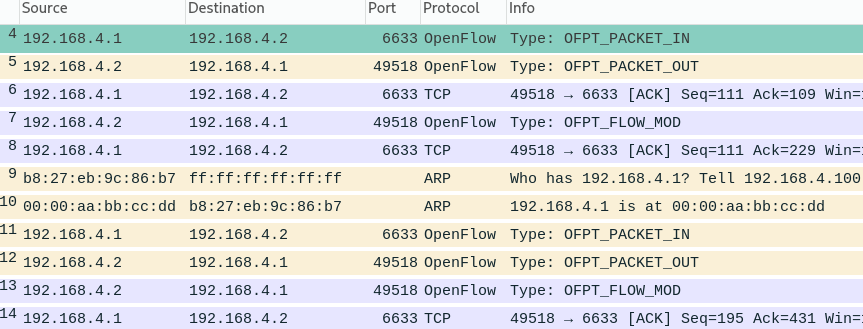
\includegraphics[scale=0.44]{../tests/RTT/newflowrule.png}
	\caption{Exp 2: Wireshark Adding New ARP Flow Rule}
	\label{fig:wireflow}
\end{figure}

As the proposed system actively installs flow rules for ARP packets,
the RTT of \emph{96.52ms} is expected as the packet is added to the flow rules and verified.
The next ARP packet sent travels with an \emph{existing flow rule}, therefore, expected to be around \emph{46.60ms} due to 
not triggering a \emph{PacketIn} event and being forwarded by the switch as seen in Figure \ref{fig:wireflowDone}.
Appendix \ref{app:rttcap} contains the entire pcap file demonstrating the lack of \emph{PacketIn} and OpenFlow
communication once a flow rule is installed.

\begin{figure}[H]
	\centering
	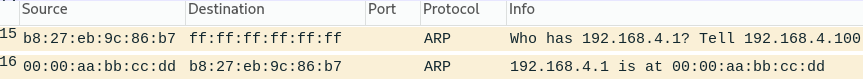
\includegraphics[scale=0.44]{../tests/RTT/newflowruleDone.png}
	\caption{Exp 2: Wireshark Verified ARP Flow Rule Exists}
	\label{fig:wireflowDone}
\end{figure}

The RTT for the proxy server is on average \emph{125.94ms}, 212\% slower than the baseline RTT. 
The results indicate a large overhead to RTT for ARP requests forwarded to the ARP proxy.
The increased RTT is due to two
factors. Firstly, the ARP reply and request packets have an extra path to traverse to reach the proposed IDPS, the extra forwarding
slows down the ARP packet. Secondly, the 
Python3 library \emph{scapy} was used to create and send the ARP reply rather than the intended ARP module service, \emph{Scapy} pulls
the ARP packet out of the Link-Layer to manage in Python which slows the response.


Figure \ref{fig:rttfull} is a comparison line chart for the four scenarios that RTT was taken. Better illustrating the minimal
affect the proposed system with a \emph{2.6\%} increase for RTT has compared to traditional networks.
Furthermore, the Figure shows the sporadic RTT that was captured for the proxy server scenario.
All RTT results are available in Appendix Section \ref{app:Exp2}.

\begin{figure}[H]
	\centering
	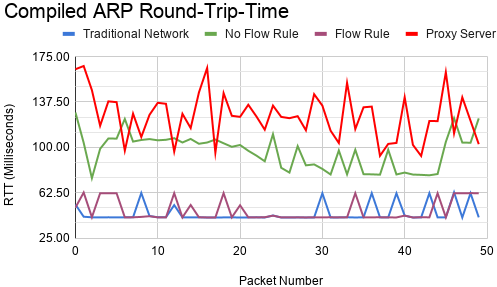
\includegraphics[scale=0.78]{../tests/RTT/ARP_RTT_full.png}
	\caption{Exp 2: Full Round-Trip-Time Comparison Line Chart}
	\label{fig:rttfull}
\end{figure}

% % % % % % % % % % % % % % % % % % % % % % % % % % % % % % % % % % % % % % % % % % % % % % % % % % % % % % % %
\newpage
\section{Experiment 3: CPU Overhead}
Experiment 3 was performed to evaluate the overhead imposed by the IDPS. The proposed IDPS aimed to reduce CPU 
overhead by actively installing flow rules, avoiding the constant CPU usage of validating ARP
packets.
The experiment measured the average CPU load of the controller and during several scenarios, this was performed
on the implemented testbed containing a RaspberryPi4 as the SDN Ryu Controller.

\subsection{Experiment Setup}
Similar to the prior experiment relying on the custom testing tool to generate results, this round ran on the \emph{phy-ryu-controller}
instead. The tool gathers the CPU load for the Ryu Controller and IDPS system 
at regular intervals during three different scenarios:

\begin{itemize}
  \itemsep0em 
  \item \textbf{Idle system:} The CPU load of the RPI4 running without the IDPS functioning, acting as a baseline.
        Therefore, no SDN traffic is being forwarded and IDPS not running on the controller.
  \item \textbf{IDPS system:} The CPU load of the IDPS functioning during normal traffic, normal ARP. This encapsulates
        DHCP server running and normal ARP messages being passed.
  \item \textbf{Proxy Server:} The CPU load as the ARP proxy is consistently replying for a blocked MAC address.
        This situation involves \emph{phy-host-one} sending an ARP request to blocked MAC address of \emph{phy-host-two},
        every \emph{1} second during testing.
\end{itemize}

\subsection{Measurements}
As stated this experiment gathers the RaspberryPi4 CPU load of the SDN controller,
the testing tool calculates the average CPU load from the four CPU core's every \emph{10} seconds for a total of \emph{15} minutes.

\subsection{Results \& Analysis}
\label{subsec:cpuload}
The results displayed in Table \ref{table:cputable} contain the Average, Minimum and Maximum CPU loads for each scenario.
It is evident from the results that the CPU load during the functioning of the IDPS is negligible, increasing on average
from \emph{0.22\%} to \emph{0.3\%}. These values show a success in the minimal resource load the IDPS consumes.
However, the ARP proxy functionality has a significant impact on the CPU load, increasing the load on average by 
\emph{24.3\%}. The significant increase in CPU load during ARP proxy replies
is likely due to the mix of running on a relatively low powered CPU, and the 
Python library \emph{scapy} was used to handle the ARP replies.

\begin{table}[H]
	\centering
	\begin{tabular}{|c|c|c|c|}
		\hline
		\rowcolor[HTML]{9B9B9B} 
		\textbf{Scenario}                                                                       & \textbf{\begin{tabular}[c]{@{}c@{}}Average CPU\\ load\end{tabular}} & \textbf{\begin{tabular}[c]{@{}c@{}}Minimum CPU\\ Load\end{tabular}} & \textbf{\begin{tabular}[c]{@{}c@{}}Maximum CPU\\ Load\end{tabular}} \\ \hline
		\cellcolor[HTML]{C0C0C0}\textbf{Idle}                                                   & 0.22\%                                                              & 0.1\%                                                               & 1\%                                                                 \\ \hline
		\cellcolor[HTML]{C0C0C0}\textbf{\begin{tabular}[c]{@{}c@{}}IDPS\\ Running\end{tabular}} & 0.3\%                                                               & 0.1\%                                                               & 1.7\%                                                               \\ \hline
		\cellcolor[HTML]{C0C0C0}\textbf{\begin{tabular}[c]{@{}c@{}}Proxy\\ Server\end{tabular}} & 24.5\%                                                              & 0.2\%                                                               & 25.9\%                                                              \\ \hline
		\end{tabular}
	\caption{Exp 3: Avg/Min/Max RTT in Each Scenario}
	\label{table:cputable}
\end{table}

Figure \ref{fig:allcpu} are the results for each test reading per scenario, the
stacked Figure \ref{fig:combinedCPU} is a stepped chart that visually demonstrates the vast difference in CPU load between
the scenario's Idle and IDPS to the proxy server. It is unlikely in the given testbed that the ARP proxy would  be replying every second.
However, these results indicate it is unlikely to expect the proposed IDPS ARP proxy to function in a
large network.

\begin{figure}[H]
	\centering
	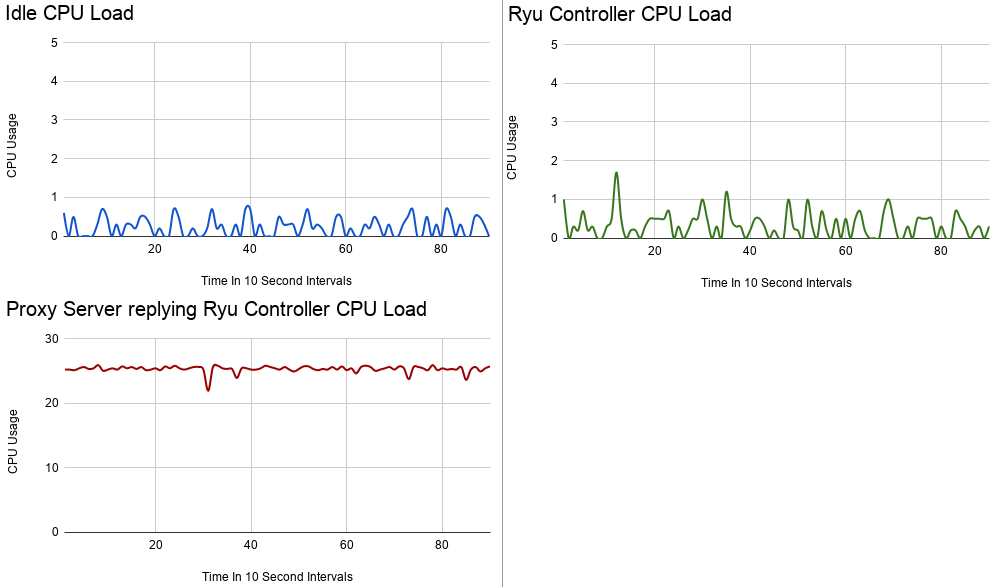
\includegraphics[scale=0.3]{../tests/CPU/allthreehoriz.png}
	\caption{Exp 3: CPU Load Charts, Avaiable in Appendix \ref{app:Exp3}.}
	\label{fig:allcpu}
\end{figure}

\begin{figure}[H]
	\centering
	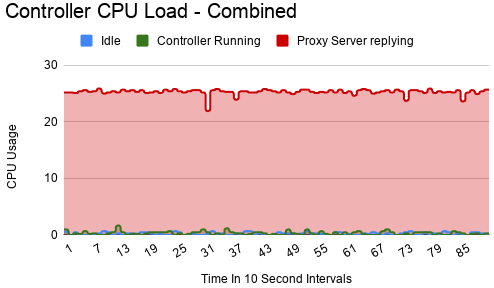
\includegraphics[scale=0.63]{../tests/CPU/allthree.png}
	\caption{Exp 3: Combined CPU Load Stepped Area Chart}
	\label{fig:combinedCPU}
\end{figure}


% % % % % % % % % % % % % % % % % % % % % % % % % % % % % % % % % % % % % % % % % % % % % % % % % % % % % % % %
% % % % % % % % % % % % % % % % % % % % % % % % % % % % % % % % % % % % % % % % % % % % % % % % % % % % % % % %
% % % % % % % % % % % % % % % % % % % % % % % % % % % % % % % % % % % % % % % % % % % % % % % % % % % % % % % %
% % % % % % % % % % % % % % % % % % % % % % % % % % % % % % % % % % % % % % % % % % % % % % % % % % % % % % % %
% % % % % % % % % % % % % % % % % % % % % % % % % % % % % % % % % % % % % % % % % % % % % % % % % % % % % % % %

\chapter{Conclusion}
The proposed IDPS emphasises and utilises the flexible capabilities of the SDN paradigm, taking advantage
of the ability to instantly drop packets and insert specifically crafted flow rules within OpenFlow 1.3.
This report demonstrates the proposed innovative hybrid IDPS tested within a physical SDN network can
detect and prevent a variety of poisoned ARP packets outlined in Table \ref{table:reqARPpos},
without impeding on the network traffic RTT.
Achieved by actively installing Link-Layer specific flow rules using the OpenFlow 1.3 protocol for 
forwarding verified ARP packets at traditional network speeds while also actively inserting flow rules which
drop blocked MAC addresses that would otherwise impede the Controller. Furthermore, the developed IDPS 
could function autonomously, generating a MAC to IP pairing by utilising the DHCP server and 
checking all unknown ARP packets; preventing the need for manual updates to the network topology.

However, the hybrid IDPS had a significant impact on the CPU load of the controller, specifically the embedded
ARP proxy server segment produced a high CPU load and increases the ARP RTT. This imposed on the SDN network, which
meant partially failure in meeting the second objective of a minimal impact on the network and minimal CPU load.

A physical testbed was implemented and configured to specifically test the developed IDPS output to reflect it's use
 in a real-world environment. Several unique tools were developed specifically 
for configuring the developed IDPS and for testing the functionality within the testbed.


\section{Limitations \& Alterantives}
The proposed IDPS has several limitations some of which were highlighted during the testing phase of the report,
while others were not as apparent. These limitations are briefly listed and explained:

\begin{enumerate}
  \itemsep0em
  \item \textbf{Scapy:} The Python3 Library \emph{scapy} is utilised to create ARP packets. This introduced a significant delay
    in receiving and sending ARP packets which was witnessed during RTT testing (Section \ref{subsec:rttres}).
    Optimisation methods were employed, yet failed to make any significant improvements.
\item \textbf{ARP Proxy:} This limitation ties into the previous, the ARP proxy produced a high CPU, load discussed in
    Section \ref{subsec:cpuload} and a large delay in RTT within Section \ref{subsec:rttres}. This was due to utilising
    \emph{scapy} for ARP packets, which when running in Python3 are slower then low-level kernel modules that usually handle
    ARP packets. The solution would be to find an alternative library or create a specific ARP packet
    library, alternatively implementing the ARP proxy in another language which runs alongside the IDPS.
\item \textbf{Limited Hardware:} The hardware used to implement the SDN network is relatively low powered and lacked certain functionality,
    such as the router not supporting SDN by default and the Raspberry Pi's using ARM Cortex processors. Ideally, the proposed IDPS
    is tested within an SDN network using a typical networking infrastructure.
\item \textbf{CSV Files:} CSV files for maintaining the lists were used out of simplicity, yet the simplicity
    has some major downsides. Firstly, the CSV files require an order and every field needs to be populated, the workaround was using the second 
    field as a Python3 Dictionary and storing the CSV files locally, therefore, only accessible by the controller and IDPS.
    Switching to a
    Structured Query Language (\emph{SQL}) database would provide a better storage format, more flexibility as well as offering 
    the advantage of being accessed by multiple SDN Controllers.
\end{enumerate}

\section{Future work}
Future iterations of the proposed system would research beyond IPv4 ARP packets, as IPv4 is slowly being decremented for IPv6.
ARP is decremented within the IPv6 address space, instead introduces the Neighbor Discovery Protocol (\emph{NDP}) which brings
many improvements over ARP. Future work would incorporate the NDP into the IDPS, bringing protection for IPv4 and IPv6 
networks, supporting a range of networks designed to function with both protocols.

The DHCP server utilisation provided by the hybrid IDPS is a dynamic approach of generating a
\emph{mac\_knownlist} and topology, however, further research could better utilise the DHCP server.
For instance when a flow rule is inserted for a verified ARP packet,
it's set with a static \emph{idle\_timeout} value; however by utilising the DHCP offer a \emph{hard\_timeout} could be 
implemented to the flow rule using the DHCP lease time. A verified flow rule could exist for the same amount of time
the DHCP lease exists for, 
minimising the frequency of times the IDPS is required to verify MAC and IP pairings.

The ARP proxy primarily functions to prevent false-positive MAC blockings by adversaries which
can effectively perform a DoS on key services. However, the performance demonstrated during testing in Section \ref{subsec:rttres} and
Section \ref{subsec:cpuload} demonstrated the partial failure of the second objective of minimal imposition on the network.
Further developmen of this report would see a redesign and rewrite of the functionality such as, implementing an ARP packet replay feature, where
the ARP proxy is not required to recreate an ARP reply every time; instead, creating an ARP reply once and replaying
the packet as required.

Further testing would ideally be performed on the IDPS, as testing was focused on functionality and the system's footprint.
However, further testing is required to measure the IDPS within a busy network to verify the effectiveness
when faced with hundreds of ARP packets per second. This report does not test for possible false-positive
MAC address blocking while proccessesng a large quantity of packets nor does it test the data throughput during these situations.


% % % % % % % % % % % % % % % % % % % % % % % % % % % % % % % % % % % % % % % % % % % % % % % % % % % % % % % %
% % % % % % % % % % % % % % % % % % % % % % % % % % % % % % % % % % % % % % % % % % % % % % % % % % % % % % % %
% % % % % % % % % % % % % % % % % % % % % % % % % % % % % % % % % % % % % % % % % % % % % % % % % % % % % % % %
% % % % % % % % % % % % % % % % % % % % % % % % % % % % % % % % % % % % % % % % % % % % % % % % % % % % % % % %
% % % % % % % % % % % % % % % % % % % % % % % % % % % % % % % % % % % % % % % % % % % % % % % % % % % % % % % %
% BIBLIOGRAPHY

% Use basic BiBTex options

	\bibliography{Bibliography}{}
	\bibliographystyle{IEEEtran}

% % % % % % % % % % % % % % % % % % % % % % % % % % % % % % % % % % % % % % % % % % % % % % % % % % % % % % % %
% APPENDIX

\appendix
\chapter{Appendix}
\section{OpenFlow}

\subsection{OpenFlow 1.0 Matching table}
\begin{table}[H]
	\begin{tabular}{|l|l|l|}
	\hline
	\rowcolor[HTML]{C0C0C0} 
	\textbf{Argument} & \textbf{Value} & \textbf{Description}                                                                                    \\ \hline
	\textbf{in\_port}          & Integer 16bit  & Switch input port.                                                                                      \\ \hline
	\textbf{dl\_src}           & MAC address    & Ethernet source address.                                                                                \\ \hline
	\textbf{dl\_dst}           & MAC address    & Ethernet destination address.                                                                           \\ \hline
	\textbf{dl\_vlan}          & Integer 16bit  & Input VLAN id.                                                                                          \\ \hline
	\textbf{dl\_vlan\_pcp}     & Integer 8bit   & Input VLAN priority.                                                                                    \\ \hline
	\textbf{dl\_type}          & Integer 16bit  & Ethernet frame type.                                                                                    \\ \hline
	\textbf{nw\_tos}           & Integer 8bit   & IP ToS (actually DSCP field, 6 bits).                                                                   \\ \hline
	\textbf{nw\_proto}         & Integer 8bit   & \begin{tabular}[c]{@{}l@{}}IP protocol or lower 8 bits of ARP\\ opcode.\end{tabular}                    \\ \hline
	\textbf{nw\_src}           & IPv4 address   & IP source address.                                                                                      \\ \hline
	\textbf{nw\_dst}           & IPv4 address   & IP destination address.                                                                                 \\ \hline
	\textbf{tp\_src}           & Integer 16bit  & TCP/UDP source port.                                                                                    \\ \hline
	\textbf{tp\_dst}           & Integer 16bit  & TCP/UDP destination port.                                                                               \\ \hline
	\textbf{nw\_src\_mask}     & Integer 8bit   & \begin{tabular}[c]{@{}l@{}}IP source address mask specified as\\ IPv4 address prefix.\end{tabular}      \\ \hline
	\textbf{nw\_dst\_mask}     & Integer 8bit   & \begin{tabular}[c]{@{}l@{}}IP destination address mask specified\\ as IPv4 address prefix.\end{tabular} \\ \hline
	\end{tabular}
	\label{table:openflow10match}
	\caption{OpenFlow 1.0 Matching table \cite{ryusdnframework}.}
\end{table}

\subsection{OpenFlow 1.3 Matching table}
\begin{longtable}{|l|l|l|}
	\hline
	\rowcolor[HTML]{C0C0C0} 
	\textbf{Argument}         & \textbf{Value} & \textbf{Description}                                                                                   \\ \hline
	\textbf{in\_port}         & Integer 32bit  & Switch input port                                                                                      \\ \hline
	\textbf{in\_phy\_port}    & Integer 32bit  & Switch physical input port                                                                             \\ \hline
	\textbf{metadata}         & Integer 64bit  & Metadata passed between tables                                                                         \\ \hline
	\textbf{eth\_dst}         & MAC address    & Ethernet destination address                                                                           \\ \hline
	\textbf{eth\_src}         & MAC address    & Ethernet source address                                                                                \\ \hline
	\textbf{eth\_type}        & Integer 16bit  & Ethernet frame type                                                                                    \\ \hline
	\textbf{vlan\_vid}        & Integer 16bit  & VLAN id                                                                                                \\ \hline
	\textbf{vlan\_pcp}        & Integer 8bit   & VLAN priority                                                                                          \\ \hline
	\textbf{ip\_dscp}         & Integer 8bit   & IP DSCP (6 bits in ToS field)                                                                          \\ \hline
	\textbf{ip\_ecn}          & Integer 8bit   & IP ECN (2 bits in ToS field)                                                                           \\ \hline
	\textbf{ip\_proto}        & Integer 8bit   & IP protocol                                                                                            \\ \hline
	\textbf{ipv4\_src}        & IPv4 address   & IPv4 source address                                                                                    \\ \hline
	\textbf{ipv4\_dst}        & IPv4 address   & IPv4 destination address                                                                               \\ \hline
	\textbf{tcp\_src}         & Integer 16bit  & TCP source port                                                                                        \\ \hline
	\textbf{tcp\_dst}         & Integer 16bit  & TCP destination port                                                                                   \\ \hline
	\textbf{udp\_src}         & Integer 16bit  & UDP source port                                                                                        \\ \hline
	\textbf{udp\_dst}         & Integer 16bit  & UDP destination port                                                                                   \\ \hline
	\textbf{sctp\_src}        & Integer 16bit  & SCTP source port                                                                                       \\ \hline
	\textbf{sctp\_dst}        & Integer 16bit  & SCTP destination port                                                                                  \\ \hline
	\textbf{icmpv4\_type}     & Integer 8bit   & ICMP type                                                                                              \\ \hline
	\textbf{icmpv4\_code}     & Integer 8bit   & ICMP code                                                                                              \\ \hline
	\textbf{arp\_op}          & Integer 16bit  & ARP opcode                                                                                             \\ \hline
	\textbf{arp\_spa}         & IPv4 address   & ARP source IPv4 address                                                                                \\ \hline
	\textbf{arp\_tpa}         & IPv4 address   & ARP target IPv4 address                                                                                \\ \hline
	\textbf{arp\_sha}         & MAC address    & ARP source hardware address                                                                            \\ \hline
	\textbf{arp\_tha}         & MAC address    & ARP target hardware address                                                                            \\ \hline
	\textbf{ipv6\_src}        & IPv6 address   & IPv6 source address                                                                                    \\ \hline
	\textbf{ipv6\_dst}        & IPv6 address   & IPv6 destination address                                                                               \\ \hline
	\textbf{ipv6\_flabel}     & Integer 32bit  & IPv6 Flow Label                                                                                        \\ \hline
	\textbf{icmpv6\_type}     & Integer 8bit   & ICMPv6 type                                                                                            \\ \hline
	\textbf{icmpv6\_code}     & Integer 8bit   & ICMPv6 code                                                                                            \\ \hline
	\textbf{ipv6\_nd\_target} & IPv6 address   & Target address for ND                                                                                  \\ \hline
	\textbf{ipv6\_nd\_sll}    & MAC address    & Source Link-Layer for ND                                                                               \\ \hline
	\textbf{ipv6\_nd\_tll}    & MAC address    & Target Link-Layer for ND                                                                               \\ \hline
	\textbf{mpls\_label}      & Integer 32bit  & MPLS label                                                                                             \\ \hline
	\textbf{mpls\_tc}         & Integer 8bit   & MPLS TC                                                                                                \\ \hline
	\textbf{mpls\_bos}        & Integer 8bit   & MPLS BoS bit                                                                                           \\ \hline
	\textbf{pbb\_isid}        & Integer 24bit  & PBB I-SID                                                                                              \\ \hline
	\textbf{tunnel\_id}       & Integer 64bit  & Logical Port Metadata                                                                                  \\ \hline
	\textbf{ipv6\_exthdr}     & Integer 16bit  & IPv6 Extension Header pseudo-field                                                                     \\ \hline
	\textbf{pbb\_uca}         & Integer 8bit   & \begin{tabular}[c]{@{}l@{}}PBB UCA header field\end{tabular}  \\ \hline
	\textbf{tcp\_flags}       & Integer 16bit  & TCP flags (EXT-109 ONF Extension)                                                                      \\ \hline
	\textbf{actset\_output}   & Integer 32bit  & \begin{tabular}[c]{@{}l@{}}Output port from action set metadata\end{tabular} \\ \hline
	\caption[An optional table caption]{OpenFlow 1.3 Matching table \cite{ryusdnframework}.\label{table:openflow13match}}\\
\end{longtable}

% % % % % % % % % % % % % % % % % % % % % % % % % % % % % % % % % % % % % % % % % % % % % % % % % % % % % % % %
% % % % % % % % % % % % % % % % % % % % % % % % % % % % % % % % % % % % % % % % % % % % % % % % % % % % % % % %

\newpage
\section{Ryu IDPS Code and Snippets}
\subsection{Ryu IDPS Code}
\lstinputlisting[language=python,caption={Ryu Controller IDPS Code Python3},captionpos=b,label={app:IDPScode}]{../code/ARP_IDPS.py}
\subsection{IDPS Tool Code}
\lstinputlisting[language=python,caption={IDPS Tool Code Python3},captionpos=b,label={app:IDPStool}]{../code/ARP_IDPS_tool.py}
\subsection{MAC Knownlist Example}
\lstinputlisting[language=Bash,caption={mac\_knownlist.csv example},captionpos=b,label={app:knownlist}]{../code/snippets/mac_knownlist.csv}
\subsection{DHCP whitelist Example}
\lstinputlisting[language=Bash,caption={dhcp\_whitelist.csv example},captionpos=b,label={app:whitelist}]{../code/snippets/dhcp_whitelist.csv}
\subsection{IDPS log Example}
\lstinputlisting[language=Bash,caption={IDPS log example},captionpos=b,label={app:idpslog}]{../code/snippets/log_20200820.csv}

% % % % % % % % % % % % % % % % % % % % % % % % % % % % % % % % % % % % % % % % % % % % % % % % % % % % % % % %
% % % % % % % % % % % % % % % % % % % % % % % % % % % % % % % % % % % % % % % % % % % % % % % % % % % % % % % %

\section{TP-Link Archer AC1750 C7 Setup}
\subsection{Network IF config}
\lstinputlisting[language=Bash,caption={OpenWRT interface config file},captionpos=b,label={app:NetworkIF}]{../code/snippets/ArcherConfig.txt}
\subsection{dnsmasq Configuration File}
\lstinputlisting[language=Bash,caption={OpenWRT dnsmasq config file},captionpos=b,label={lst:dnsmasq}]{../code/snippets/Archerdnsmasq.txt}
\subsection{Open vSwitch Configruation Setup}
\lstinputlisting[language=Bash,caption={OvS setup commands},captionpos=b,label={app:ovssetup}]{../code/snippets/OVSwitchCMD.txt}
\subsection{TP-Link Archer dnsmasq/arp clear}
\lstinputlisting[language=Bash,caption={OpenWRT DHCP clear Script},captionpos=b,label={app:dhcpclearscript}]{../code/snippets/dhcpClear.sh}

\section{NTP Configs}
\subsection{Client}
\lstinputlisting[language=python,caption={Client ntp Config file},captionpos=b,label={app:ntpclie}]{../code/snippets/ntpCli.txt}
\subsection{Server}
\lstinputlisting[language=python,caption={Server ntp Config file},captionpos=b,label={app:ntpserv}]{../code/snippets/ntpSrv.txt}


\section{Testing Tools / Code}
\subsection{IDPS Testing Tool Code}
\lstinputlisting[language=python,caption={IDPS Testing Tool Code Python3},captionpos=b,label={app:IDPStestcode}]{../code/ARP_IDPS_test.py}
\subsection{IDPS \& Testing tool log Timediff Comparison code}
\lstinputlisting[language=python,caption={IDPS \& Testing tool log Timediff Comparison code},captionpos=b,label={app:timediffcode}]{../code/Timediff.py}
\subsection{IDPS Testing Tool Help Menu}
\lstinputlisting[language=bash,caption={IDPS Testing Tool Help Menu},captionpos=b,label={app:testcodehelp}]{../code/snippets/arp_test_help.txt}


% % % % % % % % % % % % % % % % % % % % % % % % % % % % % % % % % % % % % % % % % % % % % % % % % % % % % % % %
% % % % % % % % % % % % % % % % % % % % % % % % % % % % % % % % % % % % % % % % % % % % % % % % % % % % % % % %

\section{Full Testing Results}
\subsection{Experiment 1}
\label{app:Exp1}

\begin{figure}[H]
	\centering
	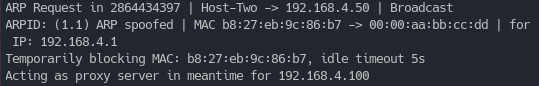
\includegraphics[scale=0.7]{../tests/a11/IDPSCap.png}
	\caption{Exp 1: ARP A1.1 IDPS Detection Log}
	\label{fig:arpa11l}
\end{figure}
\begin{figure}[H]
	\centering
	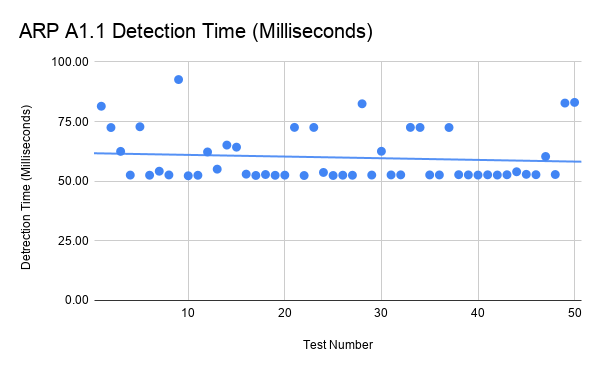
\includegraphics[scale=0.65]{../tests/aAll/ARP_A1.1_Detection_Time_(Milliseconds)_.png}
	\caption{Exp 1: ARP A1.1 Detection Time Results}
	\label{fig:arpa11g}
\end{figure}

\begin{figure}[H]
	\centering
	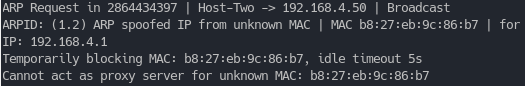
\includegraphics[scale=0.7]{../tests/a12/IDPSCap.png}
	\caption{Exp 1: ARP A1.2 IDPS Detection Log}
	\label{fig:arpa12l}
\end{figure}

\begin{figure}[H]
	\centering
	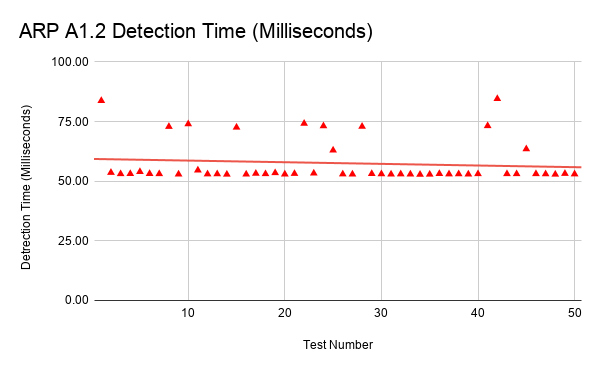
\includegraphics[scale=0.65]{../tests/aAll/ARP_A1.2_Detection_Time_(Milliseconds)_.png}
	\caption{Exp 1: ARP A1.2 Detection Time Results}
	\label{fig:arpa12g}
\end{figure}

\begin{figure}[H]
	\centering
	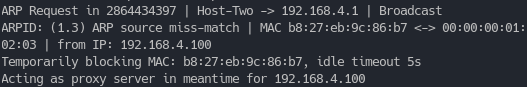
\includegraphics[scale=0.7]{../tests/a13/IDPSCap.png}
	\caption{Exp 1: ARP A1.3 IDPS Detection Log}
	\label{fig:arpa13l}
\end{figure}
\begin{figure}[H]
	\centering
	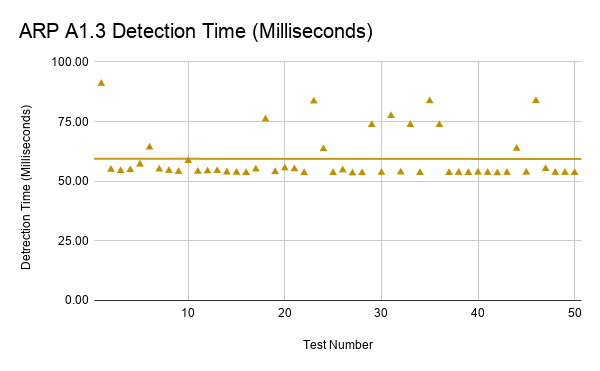
\includegraphics[scale=0.65]{../tests/aAll/ARP_A1.3_Detection_Time_(Milliseconds)_.png}
	\caption{Exp 1: ARP A1.3 Detection Time Results}
	\label{fig:arpa13g}
\end{figure}

\begin{figure}[H]
	\centering
	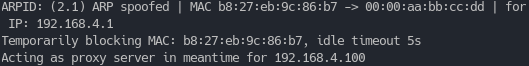
\includegraphics[scale=0.7]{../tests/a21/IDPSCap.png}
	\caption{Exp 1: ARP A2.1 IDPS Detection Log}
	\label{fig:arpa21l}
\end{figure}
\begin{figure}[H]
	\centering
	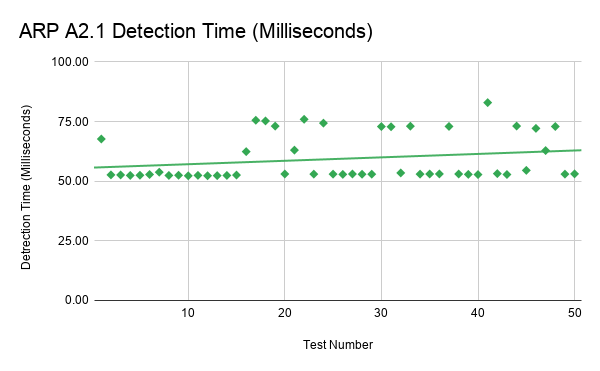
\includegraphics[scale=0.65]{../tests/aAll/ARP_A2.1_Detection_Time_(Milliseconds)_.png}
	\caption{Exp 1: ARP A2.1 Detection Time Results}
	\label{fig:arpa21g}
\end{figure}

\begin{figure}[H]
	\centering
	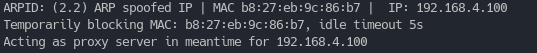
\includegraphics[scale=0.7]{../tests/a22/IDPSCap.png}
	\caption{Exp 1: ARP A2.2 IDPS Detection Log}
	\label{fig:arpa22l}
\end{figure}
\begin{figure}[H]
	\centering
	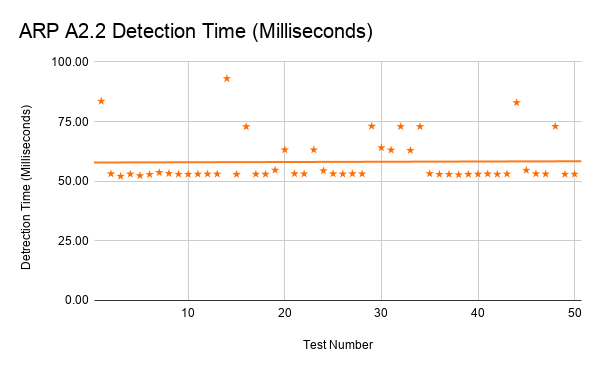
\includegraphics[scale=0.65]{../tests/aAll/ARP_A2.2_Detection_Time_(Milliseconds)_.png}
	\caption{Exp 1: ARP A2.2 Detection Time Results}
	\label{fig:arpa22g}
\end{figure}

\begin{figure}[H]
	\centering
	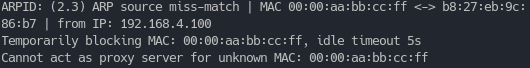
\includegraphics[scale=0.7]{../tests/a23/IDPSCap.png}
	\caption{Exp 1: ARP A2.3 IDPS Detection Log}
	\label{fig:arpa23l}
\end{figure}
\begin{figure}[H]
	\centering
	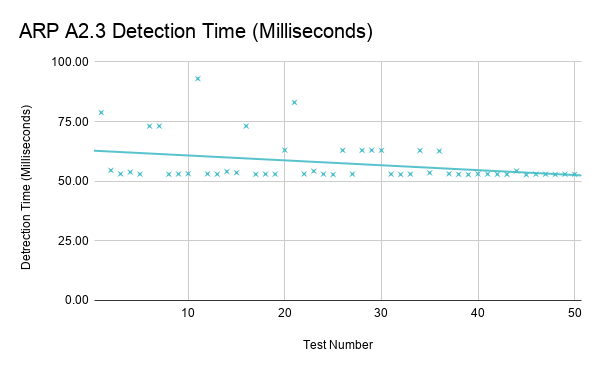
\includegraphics[scale=0.65]{../tests/aAll/ARP_A2.3_Detection_Time_(Milliseconds)_.png}
	\caption{Exp 1: ARP A2.3 Detection Time Results}
	\label{fig:arpa23g}
\end{figure}

\begin{figure}[H]
	\centering
	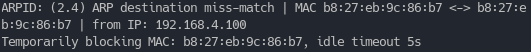
\includegraphics[scale=0.7]{../tests/a24/IDPSCap.png}
	\caption{Exp 1: ARP A2.4 IDPS Detection Log}
	\label{fig:arpa24l}
\end{figure}
\begin{figure}[H]
	\centering
	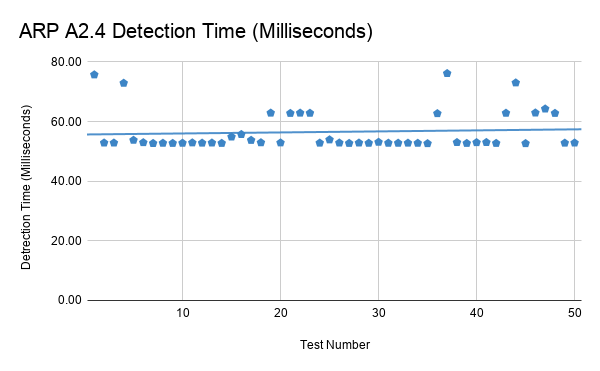
\includegraphics[scale=0.65]{../tests/aAll/ARP_A2.4_Detection_Time_(Milliseconds)_.png}
	\caption{Exp 1: ARP A2.4 Detection Time Results}
	\label{fig:arpa24g}
\end{figure}

\begin{figure}[H]
	\centering
	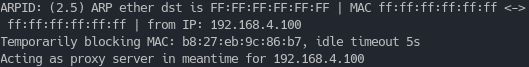
\includegraphics[scale=0.7]{../tests/a25/IDPSCap.png}
	\caption{Exp 1: ARP A2.5 IDPS Detection Log}
	\label{fig:arpa25l}
\end{figure}
\begin{figure}[H]
	\centering
	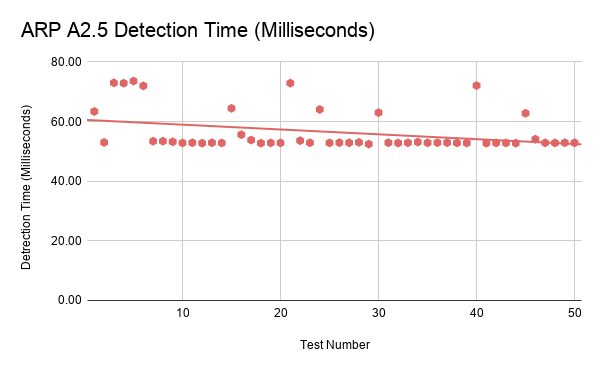
\includegraphics[scale=0.65]{../tests/aAll/ARP_A2.5_Detection_Time_(Milliseconds)_.png}
	\caption{Exp 1: ARP A2.5 Detection Time Results}
	\label{fig:arpa25g}
\end{figure}

% % % % % % % % % % % % % % % % % % % % % % % % % % % % % % % % % % % % % % % % % % % % % % % % % % % % % % % %
\subsection{Experiment 2}
\label{app:Exp2}

\begin{figure}[H]
	\centering
	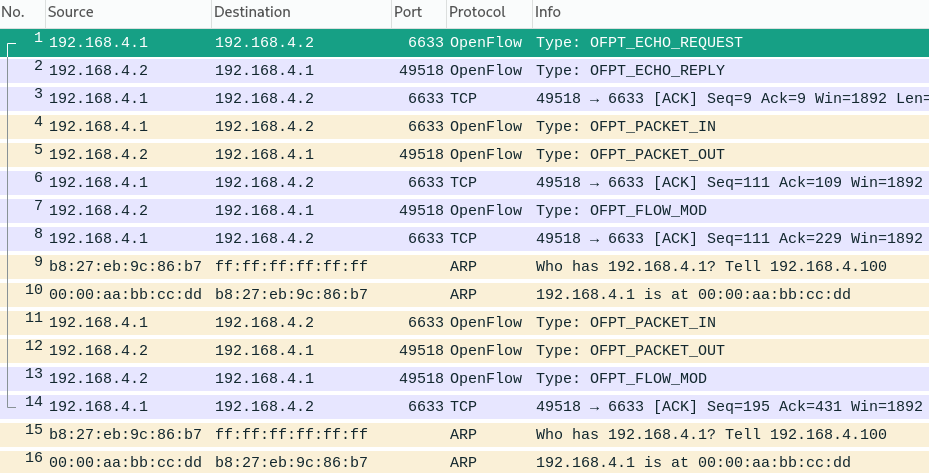
\includegraphics[scale=0.42]{../tests/RTT/newflowrulefull.png}
	\caption{Exp 2: Wireshark New and Existing ARP flow rule capture}
	\label{app:rttcap}
\end{figure}

\begin{figure}[H]
	\centering
	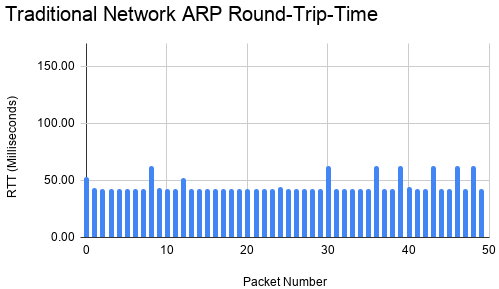
\includegraphics[scale=0.7]{../tests/RTT/TARP_RTT.png}
	\caption{Exp 2: Traditional Network ARP Round-Trip-Time Bar Chart}
	\label{fig:tarprtt}
\end{figure}

\begin{figure}[H]
	\centering
	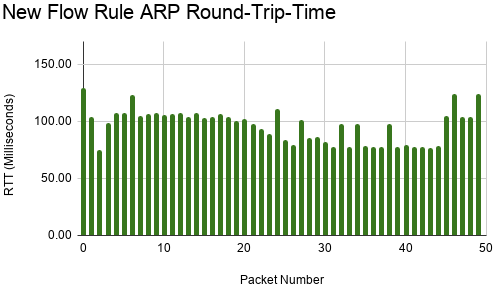
\includegraphics[scale=0.7]{../tests/RTT/NFlow_RTT.png}
	\caption{Exp 2: New ARP flow rule ARP Round-Trip-Time Bar Chart}
	\label{fig:newarprtt}
\end{figure}

\begin{figure}[H]
	\centering
	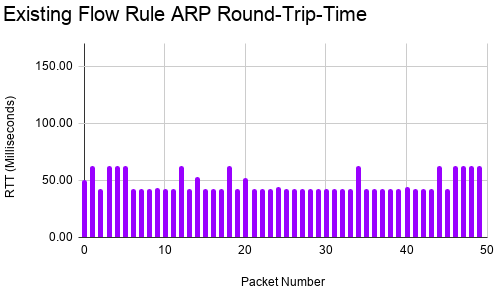
\includegraphics[scale=0.7]{../tests/RTT/EFlow_RTT.png}
	\caption{Exp 2: Existing ARP flow rule ARP Round-Trip-Time Bar Chart}
	\label{fig:exisarprtt}
\end{figure}

\begin{figure}[H]
	\centering
	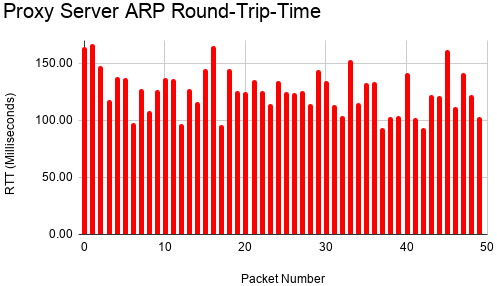
\includegraphics[scale=0.7]{../tests/RTT/PARP_RTT.png}
	\caption{Exp 2: Arp Proxy Round-Trip-Time Bar Chart}
	\label{fig:proxyrtt}
\end{figure}

% % % % % % % % % % % % % % % % % % % % % % % % % % % % % % % % % % % % % % % % % % % % % % % % % % % % % % % %

\subsection{Experiment 3}
\label{app:Exp3}

\begin{figure}[H]
	\centering
	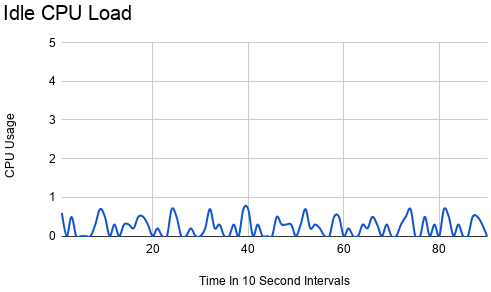
\includegraphics[scale=0.78]{../tests/CPU/idleCPU.png}
	\caption{Exp 3: Idle CPU Usage Line Chart}
	\label{fig:idlecpu}
\end{figure}

\begin{figure}[H]
	\centering
	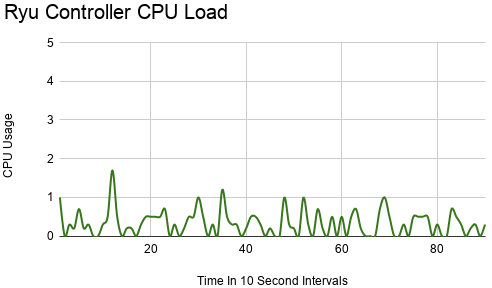
\includegraphics[scale=0.78]{../tests/CPU/useCPU.png}
	\caption{Exp 3: Ryu Controller Usual CPU Usage Line Chart}
	\label{fig:controllerCPU}
\end{figure}

\begin{figure}[H]
	\centering
	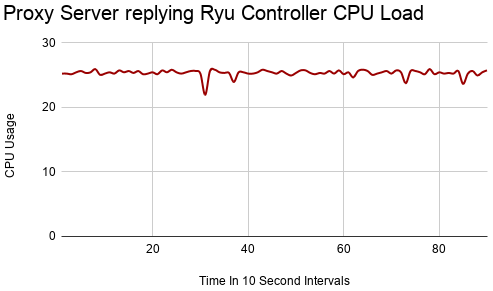
\includegraphics[scale=0.78]{../tests/CPU/proxyCPU.png}
	\caption{Exp 3: ARP Proxy Replying CPU Usage Line Chart}
	\label{fig:proxyCPU}
\end{figure}

% % % % % % % % % % % % % % % % % % % % % % % % % % % % % % % % % % % % % % % % % % % % % % % % % % % % % % % %
\end{document}
